\documentclass{article}

\usepackage{arxiv}

% --- Packages ----------------------------------------------------------
\usepackage[T1]{fontenc}
\usepackage[utf8]{inputenc}
% Use the default Computer Modern (no lmodern dependency).
\usepackage{amsmath,amssymb,amsthm}
\usepackage{mathtools}
% microtype with expansion disabled (CM doesn't support font expansion)
\usepackage[expansion=false,protrusion=false]{microtype}
\usepackage[round,authoryear]{natbib}
\usepackage{enumitem}
\usepackage{booktabs}
\usepackage{tabularx}     % for the glossary tables in §2.9
\usepackage{xcolor}
\usepackage[hidelinks,colorlinks=true,urlcolor=blue!60!black,
            linkcolor=black,citecolor=blue!50!black]{hyperref}
\usepackage{siunitx}
\usepackage{graphicx}
% Figures: regenerated PDFs live in ./figures/ (produced by the
% scripts in simulations/); hand-drawn sketches and the canonical
% Inkscape architecture diagram live at the project root.
\graphicspath{{figures/}{diagrams/}{./}}
\usepackage{caption}
\usepackage{qrcode}
\usepackage{tikz}
\usetikzlibrary{arrows.meta,positioning,calc,shapes.geometric}

% Looser float placement so wide figures don't strand themselves on a
% half-empty page. Defaults (textfraction=0.2, topfraction=0.7,
% bottomfraction=0.3, floatpagefraction=0.5) are conservative for a
% paper with several large figures.
\renewcommand{\textfraction}{0.05}
\renewcommand{\topfraction}{0.95}
\renewcommand{\bottomfraction}{0.95}
\renewcommand{\floatpagefraction}{0.85}
\usepackage{subcaption}
\usepackage{rotating}    % for sidewaysfigure (landscape, one-per-page)
\captionsetup{font=small,labelfont=bf,labelsep=period,
              skip=4pt,margin=8pt}
\captionsetup[sub]{font=small,labelfont=bf,labelsep=period}
\usepackage{placeins}    % for \FloatBarrier

% --- Theorem-like environments ----------------------------------------
\newtheorem*{definition*}{Definition}
\newtheorem*{remark*}{Remark}
\newtheorem*{claim*}{Claim}

% --- Custom macros -----------------------------------------------------
\newcommand{\caz}{\textsc{caz}}
\newcommand{\smn}{\textsc{smn}}
\newcommand{\bap}{\textsc{bap}}
\newcommand{\hap}{\textsc{hap}}
\newcommand{\nap}{\textsc{nap}}
\newcommand{\tap}{\textsc{tap}}
\newcommand{\sm}{\textsc{sm}}
\newcommand{\cns}{\textsc{cns}}
\newcommand{\Eq}[1]{Eq.~(\ref{#1})}
\newcommand{\fig}[1]{Fig.~\ref{#1}}
\newcommand{\note}[1]{\textcolor{blue!60!black}{\textsf{[Note: #1]}}}

\title{The Sensation Modulating Network:\\
Haltability as the architectural ground for object-directed
phenomenology}
\shorttitle{The Sensation Modulating Network}
\author{
G.~Nagarjuna\thanks{Email: \texttt{nagarjuna@iiserpune.ac.in};
ORCID: \url{https://orcid.org/0000-0001-6773-8454}}\\
\small Indian Institute of Science Education and Research (IISER) Pune, India
\and
Durgaprasad Karnam\thanks{Email: \texttt{karnamdpdurga@gmail.com};
ORCID: \url{https://orcid.org/0000-0002-7620-0223}}\\
\small Centre for Educational Technology (CET), Indian Institute of Technology Bombay, India
}
\date{}

% =====================================================================
\begin{document}
\maketitle

\begin{abstract}
Cognitive science remains split between cognitivism --- which
accounts for recursion and language but cannot ground formal
symbols in meaning --- and 4E approaches --- which ground
cognition in the body but rarely specify the body's
architecture in enough detail to support generativity.  We
argue the impasse stems from an incomplete account of the
embodied agent's architecture, and propose one: the
\emph{Sensation Modulating Network} (SMN), the cognitive agent
conceived as the whole body, organized at every anatomical
scale by \emph{opponent} dynamics, built from \emph{Sensation
Modulators} that sense and act through one substrate, paired
into \emph{Coordinated Action Zones} routed by a body-wide
broadcast network.  Three architectural commitments give the
SMN its purchase.  \emph{Haltability} --- the active recruitment
of antagonistic affordance into co-activated equilibrium ---
provides the architectural locus that object-directed
phenomenology, in Husserl's sense, requires: opponency makes
co-activation available, co-activation makes halt possible,
halt makes attention possible, attention makes intentional
directedness possible, with no module added on top.  The
\emph{dual-signal property} of self-modulatable action patterns
(SMAPs) renders the self/world distinction a structural feature
of the wiring rather than a category the agent applies.  And
the four-level action-pattern hierarchy --- Basal, Haltable,
Negotiable, Transactional --- gives a single architectural
trajectory from autonomic regularity to public
conventionalization, with the conditions for grammar-grounded
generativity locatable as architectural transitions.  The SMN's
position on the cognitivism--4E debate is reconciliatory:
recursion lives in the modifiable modular dynamics of
Negotiable Action Patterns; embodiment lives in the opponent
substrate that supports them.

The architecture is presented in descriptive form across the
body of the paper.  Its formal counterpart --- component
definitions, single-zone dynamics, the multi-zone network, and
eight predicted registers (seven testable, one explicitly
hypothetical: inter-body shared intentionality) together with
reference simulations realizing each register --- is stated in
an appendix. The registers are concrete
discriminators that controller--plant decompositions,
hierarchical generative models, and unstructured-substrate
accounts cannot reproduce without further commitments; each is also a
fingerprint of a dispositional state of the agent, providing a
read of the architecture as a substrate for phenomenology
rather than only for behavior.
\end{abstract}

\noindent\textbf{Keywords:}
embodied AI, cognitive architecture, haltability, opponency,
sensation modulator, phenomenology

% =========================================================================
% NEW §1, §2, §3: Introduction, the SMN in evo-devo context, related work
% =========================================================================

\section{Introduction}\label{sec:intro}

\subsection*{On reading this paper}

This paper asks what an embodied cognitive agent must structurally
be, and proposes one architectural answer.  We ask the reader to
entertain four questions.  \emph{What if embodiment is not the
situation of the brain in the body, but of the brain as one organ
within a body that is itself the unit of cognition?}  \emph{What
if the muscular system is not the body's organ for implementing
behavior, but its primary organ for sensing space?}  \emph{What
if action is, before it is anything else, the means by which an
organism computes its location?}  \emph{What if intentional
cognition requires, above all, the architectural capacity to
\emph{halt} --- to hold an attentional state actively still
against ongoing dynamics?}  Grant us the alternative architecture
these questions suggest, and a number of phenomena fall into place:
the boundary between self and world, the directedness of attention,
the gap between affordance and action, the layered evolutionary
history of motor competence.  The objective of this paper is not
to demonstrate that this alternative is correct, but that it is
\emph{possible} --- that an architecture answering all four
questions in the affirmative can be specified coherently,
formalized in part, and made to do the explanatory work that
earlier programs have struggled with.  What follows is the
specification.

\subsection*{The problem}

What is the relationship between a body and a mind? The question
is ancient, but the answers available to cognitive science remain
unsatisfying. The field is marked by a long-standing tension
between two dominant programs. On one side, cognitivism ---
rooted in a nativist, information-processing paradigm --- explains
language and reasoning through amodal representations and
computational rules, often assumed to reside in the brain
\citep{Chomsky1957SyntacticStructures,Fodor1975LanguageOfThought,
Pinker1994LanguageInstinct}. On the other, 4E approaches
(embodied, embedded, enactive, extended) ground cognition in the
dynamic, situated action of the whole body within its environment
\citep{VarelaThompsonRosch1991,MaturanaVarela1980,noe_action_2004,
clark1997being,Thompson2007MindInLife}. Both perspectives recognize
the evolutionary and biological basis of cognition, but they part
ways on the role of the body: whether it is merely an implement
for brain-based processes or a constitutive ground of mental life.

The disagreement has persisted for a reason. Cognitivism can
account for the compositionality and generativity of language but
cannot explain how formal symbols acquire meaning ---
the symbol-grounding problem \citep{Harnad1990SymbolGrounding}. 4E
approaches can explain how perception and action are coupled but
have struggled to account for the recursive, compositional
structure that cognitivism rightly identifies as central to human
cognition. Neither tradition has produced a unified account that
explains both the grounded, embodied character of animal cognition
and the generative, symbolic character of human language and
culture. We argue that the impasse stems from an incomplete
understanding of the evolved biological architecture of the
cognitive agent. Cognitivism treats the body as peripheral
input/output hardware; 4E approaches invoke it as constitutive
but rarely specify its architecture in sufficient detail to
explain generativity. This paper offers an architectural model
--- one that takes the whole body, not just the brain, as the
unit of cognitive analysis.

\subsection*{The proposal}

We propose the \emph{Sensation Modulating Network} (SMN): the
cognitive agent conceived as the entire body, organized as a
network of \emph{Coordinated Action Zones} (CAZs) whose elementary
operation is the modulation of sensation through action. Every
joint and every muscle pair is organized through Sensation
Modulators that simultaneously sense and act, while sensory
surfaces participate as transducers (read-only sense organs)
coupled into the same sensation-modulating network. The nervous
system is not the cognitive engine but the plastic communication
backbone that routes signals among these distributed processing
elements.

A central architectural assumption is that action does not require
initiation from a central or distributed command. Organisms without
nervous systems already exhibit movement; isolated cardiac tissue
continues to beat rhythmically \citep{Llinas2001-xl,Levin2014MolecularBioelectricity,
Levin2023,MarderCalabrese1996PR}. The
capacity for action is intrinsic to living cells. Unless redirected
by internal or external affordances, action patterns persist. The
nervous system's primary cognitive role is therefore not to
generate action but to indispensably participate in modulating
dynamics by routing signals that alter them and to hold a shareable
state-space in the network. Cognitive science has tended to treat the body as
peripheral: an effector for the controller, a sensor array for the
brain, a scaffolding for embodied cognition. But biological bodies
are not peripheral. They are organized at every anatomical scale by
\emph{opponent} dynamics, and those opponent dynamics are where
feeling and knowing meet \citep{Damasio1999_Feeling,Damasio2010_Self,
Damasio2021_FeelingKnowing}. Sympathetic and parasympathetic
balance the autonomic state. Flexor and extensor balance every
joint. Left and right axial musculature balance posture against
gravity. Excitation and inhibition balance every cortical and
subcortical computation.

The SMN architecture is organized around a hierarchy of action
patterns with increasing degrees of modulatory freedom: Basal
Action Patterns (BAPs) --- self-sustaining, environmentally coupled
routines that consume metabolic energy but not attention; Haltable
Action Patterns (HAPs) --- action patterns that can be paused,
redirected, and recomposed, the pivot point of the hierarchy;
Negotiable Action Patterns (NAPs) --- HAPs rephased and recombined
under perceptual predicates, enabling context-sensitive coordination;
and Transactional Action Patterns (TAPs) --- NAPs that leave durable
public traces (gestures, marks, vocalizations), entering the
inter-subjective domain. The transition from BAP to TAP is the
cognitive trajectory of the organism: from a body immersed in a
habitat to a body that participates in conventionalization,
language, and culture. The full development of the typology and
its formal treatment occupies \S\ref{sec:bridge}; in this paper
we develop the architectural conditions under which the BAP--HAP
levels are stable and the NAP layer becomes reachable. The TAP
extension --- and through it, the architectural grounding of
generative grammar and symbol use --- is the subject of companion
work.

\subsection*{Specification and phenomenology}

What the embodied-cognition tradition --- from
Merleau-Ponty's lived body
\citep{Merleau-Ponty2013-vs} through Piaget's developmental
schemas \citep{Piaget1952Origins,Piaget1971BiologyAndKnowledge}, Maturana and Varela's
autopoiesis
\citep{MaturanaVarela1980,VarelaThompsonRosch1991}, Dreyfus's
critique of representationalism
\citep{Dreyfus1972,Dreyfus1992,DreyfusDreyfus1986}, and No\"e's
sensorimotor enactivism \citep{noe_action_2004} --- has generally
not provided is an architectural specification: a tractable
engineering description of what an embodied cognitive agent must
structurally be. This paper offers such a specification,
biologically inspired but not biologically constrained, intended
as a design specification for cognitive agents (artificial,
robotic, or animal), grounded in the evolutionary--developmental
biology of animal body plans
\citep{Carroll2005EndlessForms,Nielsen2012}. A consequence of
taking opponency seriously is that an SMN's default state is
\emph{self-modulation}: heart contracts, modulating intrathoracic
pressure, modulating diaphragm activity, modulating posture,
modulating vestibular input, modulating ocular reflexes that
stabilize gaze, and so on without pause. Every persistent input
to the SMN is, by default, embedded in a coordinated pattern of
self-modulation that we call a Self-Modulatable Action Pattern
(SMAP). SMAPs have the structural property that \emph{both ends}
of any modulation relation are within the SMN, with efferent
access on both. An external object, by contrast, has no efferent
stream the SMN can read. The architectural distinction between
self-modulation and world-contact is therefore the difference
between two efferent streams jointly parameterizing a sensory
channel and one efferent stream alone --- a fact about the
wiring, not a category the agent applies.

The architectural payoff that motivates the paper concerns
\emph{phenomenology}. What does an embodied system need in order
to support object-directed phenomenology in Husserl's sense
\citep{Husserl1900_LU,Husserl1913_Ideas}? The answer this paper
develops is: \emph{haltability}. Without gaps in action ---
without the architectural ability to halt and attend --- there
is no agent capacity to hold something as available,
interruptible, and resumable, and therefore as aboutable. The
claim is structural rather than metaphysical: haltability
provides the architectural locus the phenomenological tradition's
notion of intentional directedness needs, not that haltability
\emph{produces} phenomenology. The chain runs through the
architecture --- opponency makes co-activation available;
co-activation makes halt possible; halt makes attention
possible; attention makes intentional directedness possible ---
not through any module added on top. The eight registers we
catalogue in \S\ref{sec:registers} are behavioral fingerprints
of this dispositional architecture, providing a read of the
architecture as a substrate for phenomenology rather than only
for behavior.

\subsection*{Plan of the paper}

\S\ref{sec:smn-evodevo} introduces the SMN as a layered
opponency-grounded architecture in evolutionary--developmental
context, and explains why this view of the substrate differs from
the more standard treatment of the body as either an effector for
a central controller or as an unstructured reservoir whose
dynamics happen to be useful.  \S\ref{sec:formalism-kind} states
the six architectural commitments the rest of the paper develops.
\S\S\ref{sec:dpu}--\ref{sec:network} present the architecture in
descriptive terms: zones and the Sensation Modulator, the
Coordinated Action Zone with its haltability operator,
transducers and the reafference principle, self-modulatable
action patterns and the dual-signal property, the
phase-oscillator description of CAZ networks, and the multi-CAZ
broadcast network specified as a hybrid graph-dynamical system.
The formal counterpart of each architectural section --- the
equations, the parameter dependencies, the SMN tuple, the eight
predicted registers, and the reference-simulation realizations
--- lives in \ref{app:formalism}, cross-referenced at
each architectural commitment.  The body is written for readers
who want to follow the architectural argument from question to
register without parsing equations; the appendix is written for
readers who need the mathematical statement.
\S\ref{sec:related} situates the architecture in relation to
existing accounts in cognitive science, philosophy of mind, and
cognitive robotics --- a comparison placed after the
architectural development so that affinities and substantive
differences can be stated against structural commitments rather
than against forward-pointers.  \S\ref{sec:conclusion} concludes
with what the paper has delivered, why it might warrant
consideration, and what is deferred to the companion program.

Two appendices follow the conclusion.
\ref{app:formalism} (\emph{Tentative Formalism and Results of
Simulations}) is the formal counterpart to the main body, with the
architectural dynamics stated as equations, the
reference-simulation outputs reported register-by-register, and
the implementation-design choices that realize the architecture in
code.  \ref{sec:simrepo} is a pointer to the open-source code
repository \texttt{SMN-Hydrogen}
(\url{https://github.com/gnowgi/SMN-Hydrogen}), which releases the
reference simulation code under GPL~v3 with a short note on the
repository's name and on what the code does and does not exhibit.

% =========================================================================

\section[The SMN in evolutionary--developmental context]%
{The Sensation Modulating Network in \\
evolutionary--developmental context}\label{sec:smn-evodevo}

This section introduces the SMN architecture from first principles.
The aim is to show that each architectural commitment we will
formalize in \S\S\ref{sec:dpu}--\ref{sec:network} is biologically
motivated rather than stipulated, and that the SMAP-default of
\S\ref{sec:smap} follows from the architecture rather than being
imposed on it.

\subsection{Opponency at every scale of organization}\label{sec:opponency}

The biological body is organized by opponent dynamics at every
scale at which it is organized. We list the principal layers
without attempting completeness.

\paragraph{The biochemical and homeostatic layer.}
Below the autonomic, every cell maintains itself through opponent
metabolic dynamics. Anabolic and catabolic pathways oppose each
other: protein synthesis against proteolysis, glycogen storage
against glycogenolysis, lipogenesis against lipolysis, bone
deposition against resorption. Endocrine regulation is a tissue of
opponent dyads: insulin against glucagon, parathyroid hormone
against calcitonin, thyroid hormone against its peripheral
attenuation. Ionic homeostasis runs on opponent transporters
maintaining $\mathrm{Na^+\!/K^+}$, $\mathrm{Ca^{2+}}$, and pH
gradients across membranes. In each case
the metabolic, hormonal, or ionic set point is the dynamic balance
of opponent processes --- not a value computed centrally and
imposed. The autonomic balance discussed below is the system-level
expression of a principle that already operates in the chemistry
of every cell.

\paragraph{The autonomic layer.}
Sympathetic and parasympathetic divisions of the autonomic nervous
system continuously balance arousal, heart rate, respiratory drive,
digestion, and pupillary diameter. The opposition is not optional
or occasional: it is the operating mode of the system, with
homeostatic set points emerging from the dynamic balance rather
than being computed and imposed
\citep{Damasio1999_Feeling,Damasio2010_Self}. Damasio's
``feeling of what happens'' is grounded in this layer: feeling is
the dynamic state of opponent autonomic balance, available to the
organism as a primary mode of self-knowledge prior to any
representational claim.

\paragraph{The motor layer.}
Sherrington's law of reciprocal innervation
\citep{Sherrington1906_IntegrativeAction,sherrington1905reciprocal}
established that every voluntary movement involves coordinated
activation of an agonist and relaxation of its antagonist, so that
flexor and extensor at any joint are jointly modulated rather than
independently controlled. The dynamic balance of opponent motor
units is what produces a stable joint posture; modulation of that
balance is what produces movement. Equilibrium-point control
\citep{Feldman1986_EquilibriumPoint,Feldman2015ReferentControl}
formalizes one consequence of this organization: the controlled
variable is the equilibrium of the opponent pair, not the activation
of either pole alone.

\paragraph{The bilateral and segmental layer.}
Locomotion in tetrapods, segmental swimming in fish, peristalsis in
molluscs and worms, undulation in lampreys all exhibit alternating
left--right opponency at the trunk level
\citep{Grillner2006Lamprey,Grillner2020PrinciplesMotorControl,MarderBucher2001CB,MarderCalabrese1996PR}. Central pattern
generators implement this opponency through reciprocal inhibition
between bilateral half-centers; the resulting dynamics produce
travelling waves or alternating gaits without external timing
signals. The same architectural principle scales: the segmental body
plan of bilateria is itself a layered opponency, with each segment's
dynamics coupled to its neighbours through anti-phase coordination.

\paragraph{The neural layer.}
Excitation--inhibition balance is a defining operating feature of
cortical and subcortical circuits, not a homeostatic by-product
\citep{MarderBucher2001CB,Marder2011VariabilityCompensationModulation,Marder2022NewInsightsSmallRhythmicCircuits}.
Perturbations of the balance produce specific behavioral and
clinical signatures. The simple ``every circuit is E/I balanced''
picture is increasingly refined by recent accounts of inhibitory
diversity and hetero-cellular sub-types: the architectural
commitment is to opponent dynamics at the layer, not to a uniform
two-population implementation of them, and finer-grained accounts
in which subtypes of interneurons enter into specific opponent
relations with each other and with pyramidal cells remain
compatible with the SMN's layer-level commitment.

The pattern is the same at every layer: the architectural primitive
is an opponent pair whose dynamics produce a balance state, and the
agent's behavior and feeling emerge from modulation of that
balance. We take this convergence across layers as the substantive
empirical observation that grounds the SMN architecture.

\subsection{The Sensation Modulator as the smallest unit of
opponency}\label{sec:smn-dpu}

Each end of an opponent pair must both \emph{sense} (register the
state of the pair as a whole, in order to maintain or modulate
balance) and \emph{act} (contribute to the dynamics that produce
the state). This is true at every layer of \S\ref{sec:opponency}.
The flexor's gamma-motor-neurone-mediated spindle reading
registers the joint angle that the flexor and extensor jointly
produce; a sympathetic ganglion's afferent feedback registers the
cardiopulmonary state that sympathetic and parasympathetic
activity jointly produce.

We formalize this dual function as a \emph{Sensation Modulator}
(SM): the smallest structural unit of the SMN. Each SM has a
\emph{mechanical interface}, through which it engages the body's
geometry (a configuration variable and an associated force), and
a \emph{messaging interface}, through which it participates in
the SMN's network of communication (an efferent activation it
receives and an afferent stream it emits). The SM is not a
modeling choice; it is what biological tissue \emph{does} at
every layer where opponency is the operating principle: the same
tissue that produces displacement also senses what the
displacement did to the sensory field --- it modulates sensation
through action. The formal specification is given in
\S\ref{sec:dpu}, and the network composed of these elementary
modulators is the eponymous \emph{Sensation Modulating Network}.

A note on terminology. We use the communication-engineering
phrase ``messaging interface'' (or, where the channel-like
character is salient, ``messaging channel'') rather than ``neural
pathway''. The architecture is implementation-neutral: an
artificial SMN realization could use any signaling substrate
(electrical, hormonal, optical, software). Using ``messaging''
keeps the architectural role primary and avoids the implication
that neurons are required for the architecture to work --- a
matter we return to in \S\ref{sec:smn-graph}. We avoid ``port''
deliberately, since it carries fixed prior connotations in
port-Hamiltonian systems theory and in electrical/sonar
``dual-port transducer'' usage that do not match the SMN's
architectural meaning of \emph{interface to a domain}.

\subsection{Each CAZ is a balance with a messaging beam}\label{sec:smn-caz}

A \emph{Coordinated Action Zone} (CAZ) is a pair of Sensation
Modulators in antagonistic relationship --- two zones $Z_+$ and
$Z_-$ whose forces oppose along a shared configuration variable
(a joint angle, a cardiac cycle phase, a breathing volume, a
postural sway angle, a phonatory aperture) --- together with a
small computational substrate, the \emph{communication board} $B$,
that routes messages between them. The CAZ is the smallest scale
at which opponency produces a coherent body-state variable that
the agent can both sense and modulate.

The image to hold in mind is a balance scale. A balance has two
pans whose positions are coupled inversely through a rigid beam:
when one pan rises, the other falls, and the equilibrium of the
system is the configuration in which the pans' loads are matched.
A CAZ behaves dynamically like a balance: forces from $Z_+$ and
$Z_-$ oppose along the shared variable; the system's equilibrium
is the configuration in which the two are matched; modulating one
end displaces the equilibrium predictably. The instrument-like
calibration that physical balances exhibit --- their sensitivity,
their reliability, the inverse-functional relationship that makes
them well-behaved measurement devices --- is recovered for the CAZ
because of the same opponent inverse coupling.

There is one consequential disanalogy. A balance's beam is a rigid
mechanical object; the inverse coupling of the pans is implemented
in the physical geometry of the beam. A CAZ has no such mechanical
beam. Even when $Z_+$ and $Z_-$ are anatomically adjacent --- the
flexor and extensor of the same finger, sharing the same forearm
--- they are not mechanically coupled the way the pans of a
balance are. Their dynamic balance is not produced by their
proximity but by the board $B$, which routes the message each
zone emits to its opponent partner, supplying the reciprocal
activation that each zone receives.
\textbf{The board is the beam of the CAZ-balance, but the beam is
informational rather than physical.}

This is the architectural point that distinguishes the SMN from a
literal mechanical model. The CAZ generalizes the balance principle
to systems whose opponent coupling is mediated through messages
rather than through rigid geometry. This generalization is what
makes the architecture \emph{cognitive} rather than merely
mechanical: an informational beam can be re-routed, re-weighted,
gated, or modulated in ways a rigid beam cannot. A physical
balance's beam cannot rewire itself; the SMN's board can. This is
where learning, adaptation, and context-sensitivity enter the
architecture --- not as additional machinery added to a mechanical
substrate, but as the natural operating mode of a balance whose
beam is a messaging substrate.

We will see later (\S\ref{sec:H}) that haltability --- the active
holding-still that distinguishes coordinated stopping from passive
relaxation --- is a function of the antagonism between $Z_+$ and
$Z_-$. The board does not generate haltability; antagonism does, by
making available a state of co-active equilibrium in which forces
cancel. The board's role is to recruit this affordance: to put the
system into the co-activated state, maintain it against
perturbation, and release it when appropriate. The structural fact
that opponent zones afford active equilibrium is the precondition;
the board exploits the affordance.

\begin{figure}[!htbp]
\centering
\includegraphics[width=0.85\linewidth]{fig-caz-balance.pdf}
\caption{The CAZ as a balance with a messaging beam.  The two
opponent zones Z$_+$ and Z$_-$ are the pans: they exert
pull-only forces along the shared configuration of the joint
(the fulcrum at the bottom).  The communication board (the
messaging beam at the top) routes each zone's afferent signal
to its opponent partner as the reciprocal activation --- the
same message channel carries Z$_+$'s afferent upward and
Z$_-$'s activation downward, and symmetrically on the other
side.  The board is not a rigid mechanical link --- the two
zones are not mechanically coupled --- but an
\emph{informational} beam: it weights, gates, and releases the
routing as the task and the haltability operator demand
(\S\S\ref{sec:caz}--\ref{sec:H}).  The misanalogy with a
physical balance is exactly this: a physical balance's beam is
rigid; a CAZ's beam is messaging.}
\label{fig:caz-balance}
\end{figure}

\subsection{Muscles as the substrate of spatial cognition}
\label{sec:smn-spatial}

A consequence of the Sensation Modulator's structure that we want
to register before describing the network is the following. The
Sensation Modulator is the only element of the SMN that produces
\emph{displacement} --- physical change of geometric configuration
in the body's reference frame and, through mechanical contact, in
the world's geometry. A transducer can register that
something is happening, but it cannot by itself register
\emph{where} anything is, because ``where'' is constituted by
displacement relative to a body-anchored frame, and only the
Sensation Modulator's mechanical interface participates in that frame.

The architectural consequence is that Sensation Modulators ---
muscles in vertebrate parlance, with their analogues at non-motor
layers (cardiac contraction displacing blood, peristalsis
displacing lumenal contents, ciliary motion displacing fluid) ---
are the necessary substrate of spatial cognition. Without
differential displacement, the sensory flow has no spatial structure
to extract; with it, spatial relations become derivable from the
joint history of efferent activations and their reafferent
consequences. The relationship is closely analogous to how the
Global Positioning System derives position from differential phase
of signals at a moving receiver: in both cases, differential change
rather than the isolated signal carries the geometric information.

A thought experiment makes the claim concrete. Consider an
organism with photoreceptors, chemoreceptors, mechanoreceptors,
gravity receptors, and a rich interoceptive sensory apparatus, but
without Sensation Modulators of any kind. A plant is the natural
biological example. The plant receives an enormous quantity of
sensory data and integrates it for slow growth responses
(tropisms), but on the SMN account plants lack the kind of
moment-to-moment body-centered spatial cognition generated by
SM-driven displacement, even though they may possess slower forms
of growth-mediated spatial responsiveness. Tropisms reorient the
plant's geometry over hours or days, but they do not constitute
moment-to-moment displacement in a body-centered reference frame;
they do not yield a spatial \emph{view} of the kind the SMN
architecture constructs. The point is not that plants have less
rich sensory data than animals, but that no amount of sensory
richness can substitute for the Sensation Modulator's contribution
to body-centered spatial construction.

The connection to the broader cognitive-science literature is
substantial. \citet{Berthoz2000_BrainSenseMovement} argues that
movement is constitutive of perception, not parallel to it ---
``the brain's sense of movement'' is the basis on which
perception's spatial content is built. \citet{OReganNoe2001Sensorimotor},
already engaged in \S\ref{sec:related-enactive}, make the related
constitutive claim that vision \emph{is} a particular kind of
action and that perception in general is mastery of how sensory
input changes under one's own action. The active-sensing literature
in vibrissal whisking \citep{MehtaKleinfeld2008}, saccadic vision
\citep{RucciVictor2015}, and echolocation
\citep{MossSurlykke2010} all instantiate the same principle in
specific modalities: structured motion is what makes spatial
structure available to the modality. The SMN account locates the
mechanism shared across these cases in the Sensation Modulator
and makes the structural prediction that a body without
Sensation Modulators lacks the SMN-specific mechanism for
constructing body-centered space through active displacement.

This argument also clarifies why transducers alone cannot ground
a self/world distinction (the question \S\ref{sec:smap} takes up).
Without Sensation Modulators, there is no body-frame to anchor
``self'' against; without a body-frame, ``world'' cannot be the
differentiable other. The body discovers itself before it
discovers objects, in the architectural sense that the SMN's
internal spatial structure is constructed from the same
SM-driven displacement mechanism that will later support its
external spatial structure.

\subsection{The SMN as a sensory--motor network}\label{sec:smn-graph}

The SMN is the network of all CAZs in the agent's body. Its
structure is most cleanly described in graph-theoretic terms.
Three kinds of nodes participate:

\begin{itemize}[itemsep=2pt]
\item \textbf{Motor tissue} --- the muscle--tendon--receptor
complexes that constitute Sensation Modulators at the motor layer.
\item \textbf{Sensors}, including the receptors embedded in motor
tissue (spindles, Golgi tendon organs, joint receptors,
baroreceptors, chemoreceptors;
\citealp{TuthillAzim2018ProprioceptionReview}) and the transducers
at the body's exterior (mechano-, photo-, chemo-, thermoreceptors
of the skin, retina, cochlea, olfactory and gustatory epithelia).
\item \textbf{Neurons}, which are the routing and processing
elements of the boards $B$ within each CAZ and of the broadcast
substrate that connects CAZs across the body.
\end{itemize}

One kind of edge: \textbf{synapses}, in the broad sense of
information-bearing channels between adjacent nodes --- chemical
synapses between neurons, neuromuscular junctions between neurons
and motor tissue, sensory-afferent terminals from receptors onto
neurons, and gap junctions where present. Edges are directional in
the sense that messages flow along them; the network as a whole is
densely cyclic.

Of the three node types, motor tissue is architecturally
distinguished as the sole spatial substrate: only motor-tissue
nodes have mechanical interfaces through which displacement enters the
body's geometry (\S\ref{sec:smn-spatial}). Sensors and neurons do
their work informationally, on signals already in the network;
motor tissue does its work geometrically, on the body itself.

The acronym ``SMN'' admits two readings, both useful. Structurally,
the SMN is a \emph{Sensory--Motor Network} --- the graph of
sensors, motor tissue, and neurons connected by synaptic edges.
Functionally, the SMN is a \emph{Sensation Modulating Network} ---
what the structural graph \emph{does}, namely modulate the agent's
sensations through coordinated action across opponent zones. The
structural reading describes the substrate; the functional reading
describes its operating principle. The two readings refer to the
same architecture seen from different angles, and in what follows
we use ``SMN'' for both, allowing context to disambiguate.

\subsubsection*{Common coding as architectural assumption}

A foundational architectural assumption underlies the SMN's
design. All signals routed through the SMN --- efferent activations,
proprioceptive afferents, exteroceptive inputs from transducers,
and broadcast contents --- must be \emph{mutually translatable
within a common operational code} at the level of board and
broadcast processing. The commitment is not to a single
neurophysiological encoding scheme; peripheral coding differs
across receptors, pathways, and timescales. The commitment is only
that whatever encodings are present must compose into a common
operational code by the time they participate in board-level
computation. This follows the common-coding tradition
\citep{Prinz1990CommonCoding,Hommel2001TEC} in treating action and
perception as sharing a substrate, and Llin\'as
\citep{Llinas2001-xl} in identifying that substrate, in
vertebrates, with action-potential dynamics.

The architectural reason is direct: if sensory streams were
preformatted into modality-specific symbols at the time of
broadcast, there would be no architectural role for a modulator
to play. The modulator's function is to construct, through
patterned action, the structure that distinguishes one stream
from another and renders each interpretable by the CAZ that
consumes it. Information lives in the \emph{pattern} of actions,
not in the actions themselves --- a commitment that the
dual-signal property (\S\ref{sec:smap}), the active-perception
filter (\S\ref{sec:smn-tuple}), and the externalization of NAP
traces as TAPs (\S\ref{sec:bridge}) all presuppose.

\subsubsection*{Coupling among CAZs: mechanical and through broadcast}

CAZs are coupled to one another in two ways. First, through the
body's geometry: pairs of CAZs that share mechanical contact (hand
and torso, foot and ground, lips and tongue) are mechanically
coupled, with each CAZ's configuration entering the other's
mechanical interface through the body's kinematic and dynamic relations.
Second, through a broadcast substrate: pairs of CAZs that do not
share mechanical contact but co-modulate common body-state variables
(cardiac and respiratory CAZs co-modulating intrathoracic pressure;
postural and ocular CAZs co-modulating gaze stability) are coupled
through neuronal pathways that broadcast each CAZ's state to the
others. Broadcast is not a different kind of edge from the synapses
within a CAZ's board; it is the same kind of edge at a different
spatial scale --- many-to-many synaptic communication through
neuronal routers.

Figure~\ref{fig:smn-layers} shows the layered organization
schematically.

\begin{figure}[!htbp]
\centering
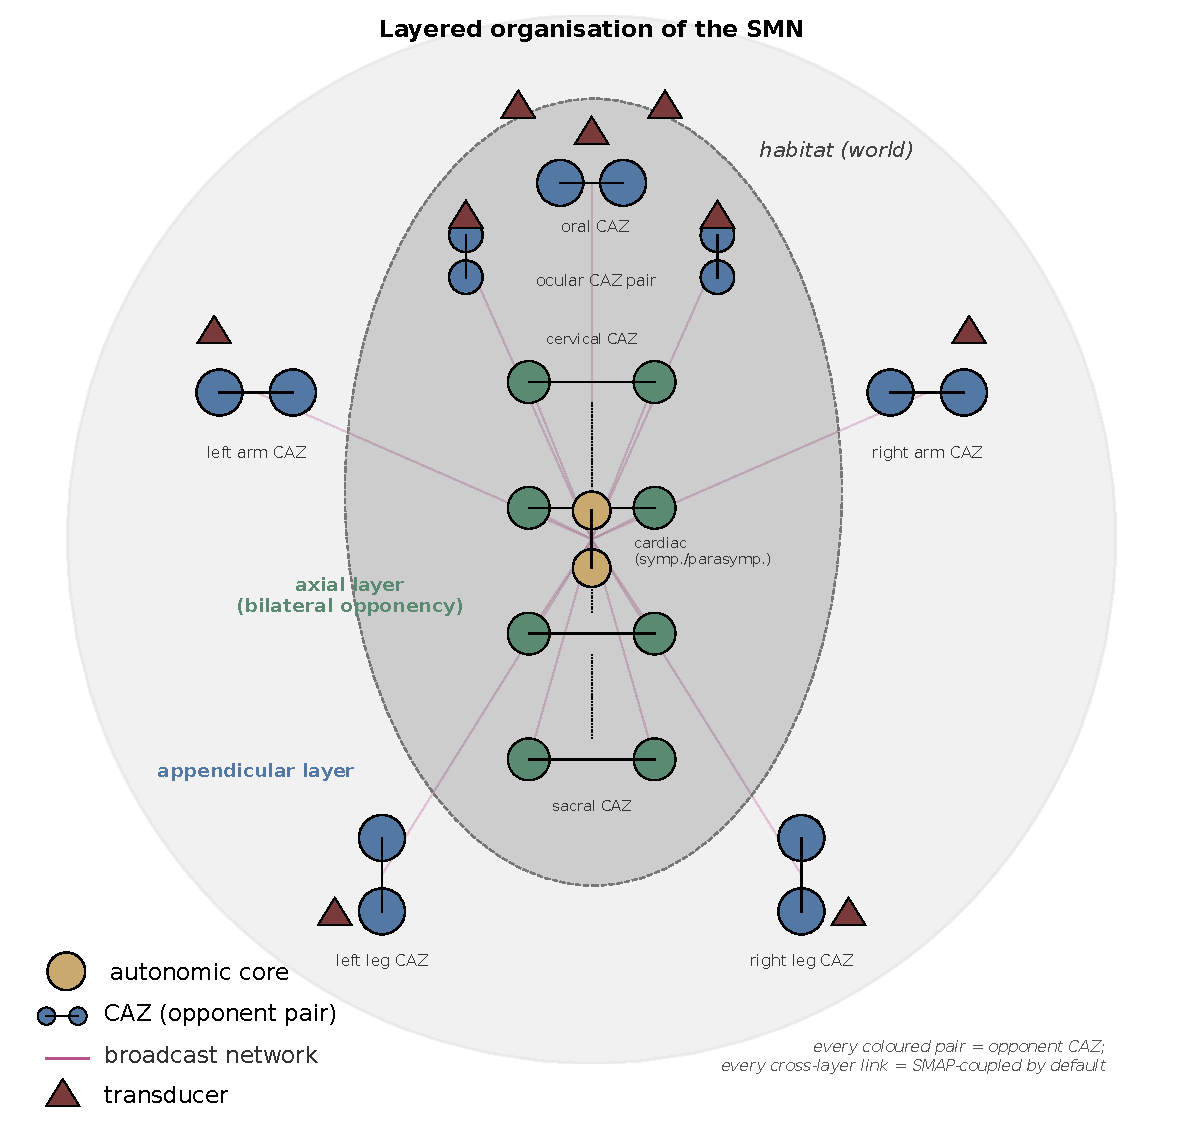
\includegraphics[width=0.86\linewidth]{smn_layered_architecture.pdf}
\caption{Layered organization of the SMN. The autonomic layer
(visceral CAZs running cardiac, respiratory, digestive cycles) sits
at the metabolic core. The axial layer (postural and locomotor
CAZs along the trunk) is bilaterally opponent and coupled to the
autonomic layer through interoceptive broadcast. The appendicular
layer (limb, oral, ocular CAZs) operates with selectable coupling
to the axial layer, allowing dexterous decoupling for manipulation.
Transducers (sense organs) deliver world-side input through the
appendicular and oral layers. Every colored connection
within the SMN is opponent (mechanical or messaging) and dual-signal
by default; the only sensory streams that lack a second efferent
counterpart within the SMN are those arriving from the habitat
through the transducer interface.}
\label{fig:smn-layers}
\end{figure}

\subsubsection*{Command is not necessary for control}

The received view in much of motor neuroscience reads efferent
direction as command: the brain decides, signals descend, muscles
execute. The SMN takes a different view, on parsimony grounds.
Contractile and signaling capacities of cells precede neurons in
evolution and persist without them: cardiac tissue in a Petri dish
beats without neural input
\citep{Marder2011VariabilityCompensationModulation}; ciliary arrays
coordinate without central direction; bioelectric signaling operates
across cellular collectives without the involvement of neurons,
both as a molecular substrate
\citep{Levin2014MolecularBioelectricity} and as a network
phenomenon
\citep{Levin2012MorphogeneticFields,LevinPezzulo2017EndogenousBioelectricNetworks};
the brain's intrinsic dynamics are the precondition rather than
the product of perceptual engagement \citep{Llinas2001-xl}. Motor
tissue is therefore not a passive effector awaiting commands; the
cells of an opponent pair already \emph{afford} active equilibrium
and do not need to be told to.

The CNS in the SMN architecture has two roles, both essential,
neither of them generative:
\begin{enumerate}[leftmargin=2em,itemsep=2pt]
\item \emph{Broadcaster}: it provides the messaging substrate
through which CAZs share state. Without broadcast the body would
be a colony of locally competent zones; with it, the body becomes
a single agent
\citep{Damasio2010_Self,Damasio2021_FeelingKnowing}.
\item \emph{State-space estimate}: it maintains an ongoing,
integrated estimate of where the body is and what it is doing,
available to every CAZ's board as context for local decisions ---
allowing local opponent dynamics to be informed by global
structure without surrendering local autonomy.
\end{enumerate}
Decentralization is therefore not in tension with the CNS but
supported by it. This is consistent with self-organization
accounts of motor coordination
\citep{Kelso1995,MarderBucher2001CB,Grillner2020PrinciplesMotorControl},
and goes further by specifying what role the CNS does play once
command is no longer assumed. The relationship with active
inference and other predictive frameworks is taken up in
\S\ref{sec:related-active-inference}.

\subsection{The asymmetries that organize the body}
\label{sec:evodevo}

A uniform substrate cannot construct geometry. A perfectly
symmetric body --- a sphere with isotropic opponent pairs ---
would have no coordinate system, because no axis would be
distinguished from any other. Coordinate systems require axes,
and axes require asymmetry. The body's specific asymmetries are
therefore not incidental anatomical facts but the substrate from
which geometric construction becomes possible.

Five asymmetries do this work, established progressively through
the evolutionary--developmental history of multicellular animals:

\begin{description}[itemsep=2pt,labelindent=0pt,leftmargin=2em,
                    style=nextline]
\item[Polarity (anterior--posterior)]
The most ancient asymmetry, present already in cnidarians. It
establishes the head--tail axis and the feeding-end / waste-end
distinction --- the preferred axis along which locomotion and
behavior are oriented.

\item[Tubularity (oral--aboral; inside--outside)]
The body has an interior tube running through it from mouth to
anus. This creates the autonomic-core / appendicular-periphery
distinction we used in \S\ref{sec:opponency}, and it makes
interoception and exteroception architecturally distinct
categories.

\item[Segmentation (rostral--caudal repetition)]
The body is laid down as a series of segments along the polarity
axis, with each segment having its own opponent organization
coupled to its neighbours through anti-phase coordination. Hox
genes pattern the segments
\citep{McGinnisKrumlauf1992Hox,Carroll2005EndlessForms}. Segmentation
is what allows locomotion to be a wave rather than a single jump,
and what allows the body's metric to be additive along the
rostral-caudal axis.

\item[Bilaterality (left--right)]
The body is mirror-symmetric across a sagittal plane, with
left-right opponent pairs at every segment. This is the symmetry
that makes the central nervous system a paired organ and that
underwrites the bilateral CAZs of \S\ref{sec:smn-caz}. Bilaterality
is what allows the body's frame to have a left-right axis, and
what enables the differential left-right reception that grounds
direction-of-arrival for many sensory modalities.

\item[Dorso-ventrality (dorsal--ventral)]
The body has a top and a bottom, with the dorsal side typically
housing the central nervous system and the ventral side typically
housing the digestive tract. This creates a gravity-aligned axis
at the body level. Dorso-ventrality is what allows the body to
have an architectural ``up'' that aligns with the gravitational
field, and what makes posture a coherent body-level variable.
\end{description}

The architectural claim is that these five asymmetries are the
\emph{constitutive substrate} of spatial cognition, in the same
way that Sensation Modulators (\S\ref{sec:smn-spatial}) are the
constitutive substrate of displacement. The Sensation Modulator
makes displacement available; the body's asymmetries provide the
axes against which displacement is meaningful. Without asymmetry,
displacement has no orientation; without orientation, no geometry.
Together, Sensation Modulators displacing along axes established
by body asymmetries are what allow the SMN to construct a geometric
model of the body and the world.

\paragraph{Asymmetry and opponency.}
This view also clarifies the relationship between asymmetry and
the opponency of \S\ref{sec:opponency}. Opponency is meaningful
only \emph{along an axis}: left--right opponency requires a
sagittal plane; flexor--extensor opponency requires a joint axis;
sympathetic--parasympathetic opponency requires the autonomic-core
axis. The body's asymmetries are what make opponency a coherent
organizing principle, by providing the axes along which opponent
pairs can be defined. Opponency at the principal anatomical layers
of \S\ref{sec:opponency} should therefore be read as opponency
\emph{along the principal anatomical axes} established by the
body's asymmetries. This is what we mean when we say the body is
not a uniform substrate populated with opponent pairs but a
substrate with definite asymmetries that establish the axes along
which opponency is meaningful.

\paragraph{The architectural payoff.}
Taken together, \S\ref{sec:smn-spatial} and the present subsection
specify what the SMN architecture is fundamentally for: it
constructs a body-anchored geometric model of the world, and
places things and events in that geometry. Cognition, on this
account, is not the manipulation of representations but the
construction and maintenance of a spatial model whose substrate
is the Sensation Modulator and whose axes are the body's
asymmetries. Concepts, language, and reasoning are built on top
of this spatial construction; they are not the foundation of it.
The remainder of the paper develops the network of CAZs that
realizes this construction.

\begin{figure}[!htbp]
\centering
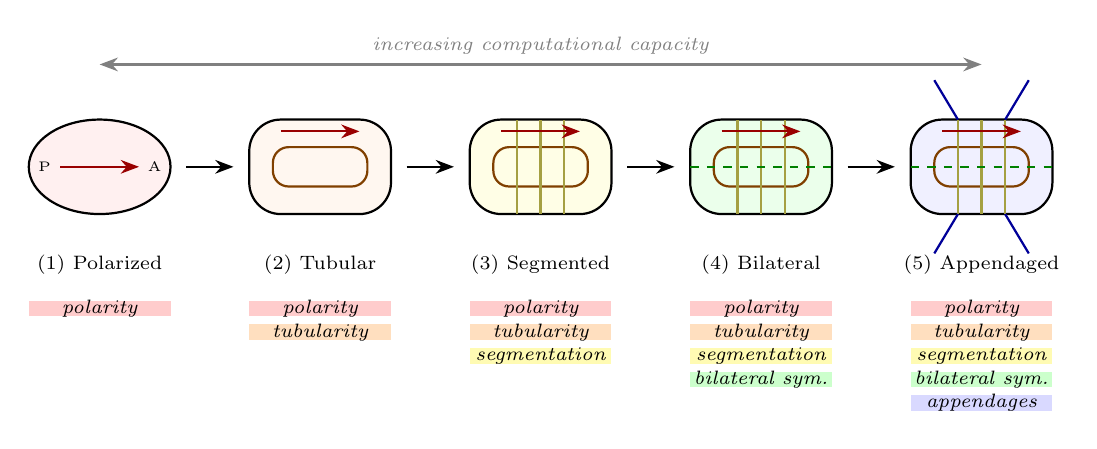
\begin{tikzpicture}[
  arr/.style={->, >=Stealth, thick},
  lbl/.style={font=\scriptsize, align=center},
  feat/.style={font=\scriptsize\itshape, text=black},
  >=Stealth
]
  \def\colsep{2.8}

  % ── Stage 1: Polarized blob ──
  \begin{scope}[shift={(0,0)}]
    \draw[thick, fill=red!6] (0,0) ellipse (0.9 and 0.6);
    \draw[thick, red!60!black, ->] (-0.5,0) -- (0.5,0);
    \node[font=\tiny] at (-0.7,0) {P};
    \node[font=\tiny] at (0.7,0) {A};
    \node[lbl, below=4mm] at (0,-0.6) {(1) Polarized};
    \fill[red!20] (-0.9,-1.9) rectangle (0.9,-1.7);
    \node[feat] at (0,-1.8) {polarity};
  \end{scope}

  \draw[arr] (1.1,0) -- (1.7,0);

  % ── Stage 2: Hollow tube ──
  \begin{scope}[shift={(\colsep,0)}]
    \draw[thick, fill=orange!6, rounded corners=4mm]
      (-0.9,-0.6) rectangle (0.9,0.6);
    \draw[thick, orange!50!black, rounded corners=2mm]
      (-0.6,-0.25) rectangle (0.6,0.25);
    \draw[thick, red!60!black, ->] (-0.5,0.45) -- (0.5,0.45);
    \node[lbl, below=4mm] at (0,-0.6) {(2) Tubular};
    \fill[red!20] (-0.9,-1.9) rectangle (0.9,-1.7);
    \fill[orange!25] (-0.9,-2.2) rectangle (0.9,-2.0);
    \node[feat] at (0,-1.8) {polarity};
    \node[feat] at (0,-2.1) {tubularity};
  \end{scope}

  \draw[arr] (\colsep+1.1,0) -- (\colsep+1.7,0);

  % ── Stage 3: Segmented tube ──
  \begin{scope}[shift={(2*\colsep,0)}]
    \draw[thick, fill=yellow!10, rounded corners=4mm]
      (-0.9,-0.6) rectangle (0.9,0.6);
    \draw[thick, orange!50!black, rounded corners=2mm]
      (-0.6,-0.25) rectangle (0.6,0.25);
    \foreach \x in {-0.3, 0, 0.3} {
      \draw[thick, yellow!60!black] (\x,-0.6) -- (\x,0.6);
    }
    \draw[thick, red!60!black, ->] (-0.5,0.45) -- (0.5,0.45);
    \node[lbl, below=4mm] at (0,-0.6) {(3) Segmented};
    \fill[red!20] (-0.9,-1.9) rectangle (0.9,-1.7);
    \fill[orange!25] (-0.9,-2.2) rectangle (0.9,-2.0);
    \fill[yellow!30] (-0.9,-2.5) rectangle (0.9,-2.3);
    \node[feat] at (0,-1.8) {polarity};
    \node[feat] at (0,-2.1) {tubularity};
    \node[feat] at (0,-2.4) {segmentation};
  \end{scope}

  \draw[arr] (2*\colsep+1.1,0) -- (2*\colsep+1.7,0);

  % ── Stage 4: Bilateral symmetry ──
  \begin{scope}[shift={(3*\colsep,0)}]
    \draw[thick, fill=green!8, rounded corners=4mm]
      (-0.9,-0.6) rectangle (0.9,0.6);
    \draw[thick, orange!50!black, rounded corners=2mm]
      (-0.6,-0.25) rectangle (0.6,0.25);
    \foreach \x in {-0.3, 0, 0.3} {
      \draw[thick, yellow!60!black] (\x,-0.6) -- (\x,0.6);
    }
    \draw[thick, dashed, green!50!black] (-0.9,0) -- (0.9,0);
    \draw[thick, red!60!black, ->] (-0.5,0.45) -- (0.5,0.45);
    \node[lbl, below=4mm] at (0,-0.6) {(4) Bilateral};
    \fill[red!20] (-0.9,-1.9) rectangle (0.9,-1.7);
    \fill[orange!25] (-0.9,-2.2) rectangle (0.9,-2.0);
    \fill[yellow!30] (-0.9,-2.5) rectangle (0.9,-2.3);
    \fill[green!20] (-0.9,-2.8) rectangle (0.9,-2.6);
    \node[feat] at (0,-1.8) {polarity};
    \node[feat] at (0,-2.1) {tubularity};
    \node[feat] at (0,-2.4) {segmentation};
    \node[feat] at (0,-2.7) {bilateral sym.};
  \end{scope}

  \draw[arr] (3*\colsep+1.1,0) -- (3*\colsep+1.7,0);

  % ── Stage 5: Appendaged ──
  \begin{scope}[shift={(4*\colsep,0)}]
    \draw[thick, fill=blue!6, rounded corners=4mm]
      (-0.9,-0.6) rectangle (0.9,0.6);
    \draw[thick, orange!50!black, rounded corners=2mm]
      (-0.6,-0.25) rectangle (0.6,0.25);
    \foreach \x in {-0.3, 0, 0.3} {
      \draw[thick, yellow!60!black] (\x,-0.6) -- (\x,0.6);
    }
    \draw[thick, dashed, green!50!black] (-0.9,0) -- (0.9,0);
    \draw[thick, red!60!black, ->] (-0.5,0.45) -- (0.5,0.45);
    \draw[thick, blue!60!black] (-0.3,0.6) -- (-0.6,1.1);
    \draw[thick, blue!60!black] (-0.3,-0.6) -- (-0.6,-1.1);
    \draw[thick, blue!60!black] (0.3,0.6) -- (0.6,1.1);
    \draw[thick, blue!60!black] (0.3,-0.6) -- (0.6,-1.1);
    \node[lbl, below=4mm] at (0,-0.6) {(5) Appendaged};
    \fill[red!20] (-0.9,-1.9) rectangle (0.9,-1.7);
    \fill[orange!25] (-0.9,-2.2) rectangle (0.9,-2.0);
    \fill[yellow!30] (-0.9,-2.5) rectangle (0.9,-2.3);
    \fill[green!20] (-0.9,-2.8) rectangle (0.9,-2.6);
    \fill[blue!15] (-0.9,-3.1) rectangle (0.9,-2.9);
    \node[feat] at (0,-1.8) {polarity};
    \node[feat] at (0,-2.1) {tubularity};
    \node[feat] at (0,-2.4) {segmentation};
    \node[feat] at (0,-2.7) {bilateral sym.};
    \node[feat] at (0,-3.0) {appendages};
  \end{scope}

  % Top annotation
  \draw[<->, thick, gray] (0,1.3) -- (4*\colsep,1.3)
    node[midway, above, font=\scriptsize\itshape, text=gray]
    {increasing computational capacity};

\end{tikzpicture}
\caption{The morphogenetic progression that scaffolds the SMN.
Each feature, once gained, persists through all subsequent stages
(shown by the cumulative colored bars beneath each diagram).
(1)~Polarity establishes a directional axis.
(2)~Tubularity creates a through-gut with haltable peristaltic
flow. (3)~Segmentation distributes CAZs along the axis.
(4)~Bilateral symmetry creates matched left--right zones.
(5)~Paired appendages add independently controllable effectors.
Each step adds computational capacity while retaining all prior
features. The progression complements the five asymmetries listed
in this section: polarity, tubularity, segmentation, and
bilaterality appear in both; the figure's fifth stage
(appendages) is best read as a downstream consequence of
bilaterality rather than as a separate axis of asymmetry, while
the section's fifth axis (dorso-ventrality) is what aligns the
appendaged body to gravity.}
\label{fig:morphogenetic-progression}
\end{figure}

% =====================================================================
% NOTE: fig:nested-morphogenetic dropped from the doc (the horizontal
% fig:morphogenetic-progression above carries the same content);
% PDF retained in diagrams/ for possible later use.
% =====================================================================

\paragraph{Evolutionary--developmental sequencing.}
The asymmetries are established progressively through evolution.
Cnidarians have polarity and dorso-ventrality but lack
bilaterality and segmentation. Bilaterians add segmentation and
bilaterality, conserved across the protostome--deuterostome split
and elaborated in vertebrates into the dorsal--ventral and
rostral--caudal axes that organize the spinal cord and brainstem.
Each evolutionary addition makes more spatial structure available
to the architecture: polarity gives forward; tubularity gives
inside-outside; segmentation gives metric along the body axis;
bilaterality gives left-right; dorso-ventrality gives up-down. By
the time a vertebrate body plan is in place, the substrate has
the full set of axes needed for three-dimensional spatial
construction in a gravitational field.

This evolutionary--developmental fact has architectural consequences
that distinguish the biological substrate from generic dynamical
systems. The body is a \emph{structured} substrate whose layered
opponency is itself the result of hundreds of millions of years of
evolutionary entrenchment, and whose asymmetries provide the
geometric axes along which that opponency becomes meaningful.
The structure is specific: definite topology (which left goes with
which right, which flexor with which extensor), definite scaling
across layers (autonomic core, axial trunk, appendicular periphery),
and definite developmental sequencing (heartbeat before breathing,
breathing before locomotion, locomotion before fine manipulation).

\paragraph{Form-as-known-from-within.}\label{sec:identity}
A consequence of the evolutionary--developmental view is that each
organism's SMN runs on \emph{its} specific body --- not a generic
body but this body's specific opponent partnerships, geometric
coupling, and broadcast topology. A bipedal vertebrate's SMN is
not the same as a cephalopod's; their respective SMAP repertoires
make different things detectable as world-residue. This is identity
formation in the structural sense: not a representational claim
about a self-concept, but the architectural claim that each
organism's form-as-known-from-within is encoded in the dual-signal
pattern of its specific SMAP repertoire. This connects to the
lived-body literature
\citep{Merleau-Ponty2013-vs,gallagher2005how,Thompson2007MindInLife}
and supplies a mechanistic substrate for the body schema as an
equilibrium of pairwise SMAP relations among CAZs.

\subsection{Open architectural questions}\label{sec:open-questions}

The architectural commitments of the preceding subsections raise
several questions that this preprint does not resolve. We gather
them here so that the body of the paper can move on without
repeated in-line caveats.

\begin{enumerate}[label=Q\arabic*.,leftmargin=2.4em,itemsep=4pt]
\item \emph{Spatial cognition without Sensation Modulators}
(\S\ref{sec:smn-spatial}). If body-centered spatial cognition
requires SM-driven displacement, what is the architectural
status of plant tropisms and other slower spatial responsiveness
in organisms lacking Sensation Modulators? The SMN architecture
identifies the moment-to-moment displacement-grounded mode but
does not adjudicate whether other modes of spatial responsiveness
deserve the term ``spatial cognition'' in some weaker sense.

\item \emph{Partial loss of the SM substrate}
(\S\ref{sec:smn-spatial}). What does the architecture predict
for embodiments where the SM substrate is partial or impaired
--- locked-in syndrome, complete spinal cord injury, advanced
neuromuscular disease? Is body-centered space gradually lost,
replaced by inferred space from preserved transducer channels, or
maintained through residual SM pathways at deeper anatomical
layers?

\item \emph{Biological scope of opponency}
(\S\S\ref{sec:opponency}, \ref{sec:evodevo}). Are there
biological layers or anatomical regions where the opponency
principle does not hold, or holds only weakly? The architecture
commits to opponency along the principal anatomical axes, not to
a literal universalism on which every micro-anatomical structure
participates in opponent dynamics. The empirical scope of the
commitment is open.

\item \emph{The metabolic interpretation of $E_R$}
(\S\ref{sec:H}). If $E_R$ is a real metabolic quantity, what does
the architecture predict about the energetic cost of attention-
driven coordination, and how would this be distinguished
empirically from the metabolic cost of motor execution itself?
The architecture commits to maintaining co-activation being
energetically expensive in a specific way; controlled experiments
on antagonist tone in primed-but-not-acting muscle groups are
the place to test it.

\item \emph{Subjectivity and the grounding of objectivity}
(\S\ref{sec:smap}). The SMN's architectural priority of
self-modulation places body-anchored construction at the
foundation of cognition and treats the discovery of the world as
a developmental achievement built on that foundation
(\S\ref{sec:roadmap}, items 1--2). Whether this view is
compatible with realist philosophical commitments or requires a
more constructivist reading is a question for downstream
philosophical work.
\end{enumerate}

% =========================================================================
% §2.10 — Glossary tables (added per review-4)
% =========================================================================

\subsection{Glossary of architectural terms}\label{sec:glossary}

The architecture's terminology accumulates across the paper.
Table~\ref{tab:gloss-arch} below gives the architectural objects
(the ``things'' the SMN is made of) as a single-place reference;
the formal operators and symbols (the variables and functions
that appear in the equations) are tabulated separately in
Table~\ref{tab:gloss-formal} of \ref{app:formalism}.

\begin{table}[h]
\centering
\small
\caption{Architectural objects.}
\label{tab:gloss-arch}
\begin{tabularx}{\linewidth}{@{}l l X l@{}}
\toprule
\textbf{Term} & \textbf{Short definition} & \textbf{Note} & \textbf{Section} \\
\midrule
SMN & Sensation Modulating Network. &
The whole-body cognitive agent: a network of CAZs across anatomical
scales, coupled by a broadcast substrate.
& \S\ref{sec:smn-graph} \\
\addlinespace[2pt]
CAZ & Coordinated Action Zone. &
Smallest unit of opponent coordination: antagonistic pair of zones
plus a communication board. A balance with a messaging beam.
& \S\ref{sec:caz} \\
\addlinespace[2pt]
SM & Sensation Modulator. &
Tissue complex that senses and acts through one substrate, with a
mechanical interface (engaging body geometry) and a messaging
interface (engaging the SMN's network).
& \S\ref{sec:dpm} \\
\addlinespace[2pt]
Zone & Sense-and-act tissue complex. &
A flexor, extensor, or analogue: any tissue that senses and acts
at one site in opponent relation to a partner.
& \S\ref{sec:zone} \\
\addlinespace[2pt]
Board & Communication board within a CAZ. &
Reads afferents, applies the halt gate, writes activations subject
to alert-energy modulation.
& \S\ref{sec:caz}, \S\ref{sec:network} \\
\addlinespace[2pt]
Transducer & Read-only sense organ. &
Converts an environmental field into a neural signal; unlike an
SM, does not write back into mechanical state.
& \S\ref{sec:transducer} \\
\addlinespace[2pt]
Broadcast & Cross-CAZ communication substrate. &
Channel by which each CAZ's state contributes to and reads from a
shared body-state estimate; mediated by $\Pi$.
& \S\ref{sec:smn-graph}, \S\ref{sec:smn-tuple} \\
\addlinespace[2pt]
SMAP & Self-Modulatable Action Pattern. &
Coordinated activation in which both modulation ends are within the
SMN. The default operating mode: every persistent input is a SMAP.
& \S\ref{sec:smap} \\
\addlinespace[2pt]
BAP & Basal Action Pattern. &
Self-sustaining, environmentally coupled routine consuming metabolic
energy but not attention (heartbeat, breathing, postural sway).
& \S\ref{sec:intro}, \S\ref{sec:network} \\
\addlinespace[2pt]
HAP & Haltable Action Pattern. &
Action pattern that can be paused, redirected, and recomposed; the
pivot of the architecture's action hierarchy.
& \S\ref{sec:intro}, \S\ref{sec:network} \\
\addlinespace[2pt]
NAP & Negotiable Action Pattern. &
A HAP rephased and recombined under perceptual predicates;
modifiable modular primitive (see \S\ref{sec:roadmap}, item~3).
& \S\ref{sec:intro}, \S\ref{sec:bridge} \\
\addlinespace[2pt]
TAP & Transactional Action Pattern. &
A NAP whose phase-reset events leave a public trace (gestures,
vocalizations, marks); locus of inter-subjective generativity.
& \S\ref{sec:intro}, \S\ref{sec:bridge} \\
\bottomrule
\end{tabularx}
\end{table}


\FloatBarrier

% =========================================================================

% =========================================================================
% Note: comparison with related work has been moved to §11, after the
% formalism and registers are in place. See \S\ref{sec:related}.
% =========================================================================


% ---------------------------------------------------------------------
\section{Architecture by commitments}\label{sec:formalism-kind}

Before we work through the architecture in detail, we want to
state plainly what it commits to.  The Sensation Modulating
Network is specified primarily by six architectural commitments
(C1--C6 below); the formal apparatus that realizes them is in
\ref{app:formalism}.  A reader who wants to see what the
architecture is and why it has the shape it does need not parse
the equations; the commitments carry the substantive content.  A
reader who wants the dynamics formalized, the variables defined,
and the reference simulations reported can find all of that in
\ref{app:formalism}, which is internally complete and
cross-referenced to the sections of the main body it formalizes.

\subsection{Six commitments of the architecture}\label{sec:axioms}

We state the six commitments below in order, numbered so that
subsequent sections and the registers can refer back to them
directly.

\begin{description}[itemsep=4pt,labelindent=0pt,leftmargin=2em,
                    style=nextline]
\item[Commitment C1 (opponency at every scale of organization)]\label{ax:opponency}
The body is organized by opponent dynamics at every scale at which
it is organized: biochemical/metabolic, autonomic, motor,
bilateral/segmental, neural, and perceptual
(\S\S\ref{sec:opponency}, \ref{sec:evodevo}). The architectural
primitive at every scale is an opponent pair whose dynamics
produce a balance state. This is not a parsimonious modeling
choice; it is the substantive empirical observation that grounds
the architecture.

\item[Commitment C2 (Sensation Modulators everywhere)]\label{ax:dualport}
The smallest structural element of the SMN is the Sensation
Modulator (SM): a single tissue complex that both senses and acts
through one substrate, with a mechanical interface engaging body
geometry and a messaging interface engaging the SMN's network
(\S\ref{sec:dpu}). The architecture is implementation-neutral
about what carries the messages, but commits to the structural
fact that sensing and acting share a substrate.

\item[Commitment C3 (decentralized coordination through broadcast)]\label{ax:broadcast}
The architecture is decentralized: each CAZ runs its own balance
computation locally, using its own SM afferents and the
broadcast it reads from the rest of the body. Coordination is a
property of the network, not a function the network computes
(\S\ref{sec:smn-graph}). The CNS, on this account, supports
decentralization by maintaining shared state-space rather than
overriding it.

\item[Commitment C4 (active-perception filtering: drop if not acted upon)]\label{ax:alpha}
Each CAZ's communication board attends only to sensor streams
currently coupled to that CAZ's modulation. Streams whose
variation is not predicted by the local reafference predictor as
a consequence of current efferent activity are dropped from the
board's predictive computation. This is a parsimony commitment:
with a body producing far more sensory data than any local
computation can attend to, the architecture's solution is to
filter at ingress, admitting only what is currently acted upon.
The filter $\alpha$ is not total blindness: streams not in
$\alpha$ remain under low-cost peripheral monitoring whose role is
to register signal-level changes that may warrant promotion to
board-level attention. The architecture distinguishes two stages:
peripheral monitoring (always running on every stream, low cost,
no predictive computation) and board-level admission (the gated
subset $\alpha$ that enters the board's predictive computation).
The filter is stated formally in \S\ref{app:formal-network} as
the active-perception filter $\alpha$ in the SMN tuple, in
consonance with active-perception accounts
\citep{Bajcsy1988_ActivePerception,OReganNoe2001Sensorimotor}.

\item[Commitment C5 (habituation: drop the predictable)]\label{ax:habituation}
Streams that are coupled to current modulation but whose variation
is fully predicted by an ongoing BAP --- heart beating,
breathing, postural sway --- drop out of attended status not
because they are uncoupled but because their coupling is fully
predicted. This is a complementary commitment to active-perception
filtering: C4 drops uncoupled streams; C5 drops coupled-but-
predicted streams. Both reduce computational load by restricting
attention to streams that carry information the predictor has not
already absorbed.

\item[Commitment C6 (spatial cognition through differential displacement)]\label{ax:displacement}
Spatial structure is constructible only from the differential
displacement that Sensation Modulators produce, registered against
the axes established by the body's developmental asymmetries
(\S\S\ref{sec:smn-spatial}, \ref{sec:evodevo}). The SMN is
fundamentally a geometric architecture: what it constructs is a
body-anchored spatial model of itself and of the world.
\end{description}

These six commitments (C1--C6) are not all of the same kind, and
the distinction matters for any reader trying to test or refute
the architecture.  Two are \emph{empirical generalizations} the
architecture takes on board (C1 on opponency, C6 on spatial
cognition) --- substantive empirical observations that ground
the architecture and that would be falsified by sustained
evidence against them.  Two are \emph{structural commitments
about elementary units} (C2 on the Sensation Modulator, C3 on
decentralized coordination through broadcast) --- architectural
moves that fix what the smallest elements of the SMN are and
how they cohere.  Two are \emph{design commitments} or parsimony
moves (C4 on active-perception filtering, C5 on habituation) ---
choices made when the architecture is instantiated, defensible
by parsimony arguments rather than by empirical inevitability.

These six commitments are what the SMN architecture commits to.
The remainder of the paper employs these commitments to specify
the architecture, to develop its formalism (in
\ref{app:formalism}), and to derive the empirical registers that
follow from them.

\paragraph*{What kind of specification this is.}
The architecture is rigorous in some places and acknowledged as
schematic in others.  Architectural definitions --- components,
relations, input/output signatures --- are fully specified for
every element we name.  Single-CAZ dynamics are specified as a
closed system of differential equations with explicit dynamical
laws and named parameters, rigorous as a toy model and
serviceable as a reference implementation design; the formal
statement is in \ref{app:formalism}.  Multi-CAZ network dynamics ---
stability, controllability, observability, convergence --- are
specified architecturally, but their analytical theory is
\emph{deferred} to future work.  We do not claim a completed
mathematical theory of SMN networks; we claim a specification of the
architectural object whose theory is to be developed.  Reference
simulations (\S\ref{sec:registers}, with details in
\ref{app:formalism}) function as existence proofs that the
specified equations can generate the predicted contrasts; they are
not claimed as biological validation.  \ref{app:formalism}
states this classification in full, alongside a map of how the
formalism's sub-systems fit together.

\begin{figure}[!htbp]
\centering
\includegraphics[width=\linewidth]{fig-smn-anatomy.pdf}
\caption{Anatomy of the SMN architecture, at three nested
scales. \emph{Left:} the Sensation Modulator (SM) --- the
elementary unit, a tissue complex that senses and acts through
one substrate, with a mechanical interface engaging body geometry
(red, downward) and a messaging interface engaging the SMN's
network (blue, sideways).  \emph{Middle:} the Coordinated Action
Zone (CAZ) --- two opponent SMs (the pans), a communication
board above (the messaging beam) that routes each zone's afferent
to its opponent partner, and the joint below (the shared
configuration the two zones pull on).  \emph{Right:} the
Sensation Modulating Network (SMN) --- many CAZs distributed
across the body, integrated by a body-wide broadcast (dashed
orange) so that every CAZ contributes to and reads from a shared
state-space.  Each level is composed from the previous by
opponent pairing and broadcast.}
\label{fig:smn-anatomy}
\end{figure}


% ---------------------------------------------------------------------
\section{Zones and the Sensation Modulator}\label{sec:dpu}

This section describes the smallest structural elements of the SMN
--- the \emph{zone} and the \emph{Sensation Modulator}.  The
formal statement of the dynamics is in \S\ref{app:formal-sm}.

\subsection{The zone}\label{sec:zone}

A \emph{zone} is one tissue complex that participates as a member
of an opponent pair.  Paradigmatically a zone is a
muscle--tendon--receptor bundle (the flexor of an elbow, the
extensor of a finger, the diaphragm, the sympathetic ganglion of a
cardiac segment), but the architectural notion is more general:
any tissue complex that both senses and acts at one anatomical
site, and stands in opponent relationship to a partner zone,
qualifies.

A zone engages the rest of the architecture through two distinct
\emph{interfaces} --- one mechanical, one informational.

The \emph{mechanical interface} is where the zone engages the
body's geometry.  It is described by two coupled variables: a
\emph{configuration} --- where the zone is along its axis of
operation (a length, a joint angle, a chamber volume, an aperture
diameter) --- and a \emph{force}, the pull the zone applies along
that axis.  Both are determined jointly by the zone's internal
state and by what the body is currently doing.

The \emph{messaging interface} is where the zone participates in
the SMN's network of communication.  It carries two messages in
opposite directions: an \emph{efferent activation} that the zone
\emph{receives} from the rest of the SMN, telling it how strongly
to engage; and an \emph{afferent signal} that the zone
\emph{emits} from its embedded receptors, reporting its mechanical
state to the rest of the SMN.

The terminology ``messaging interface'' rather than ``neural
pathway'' was introduced in \S\ref{sec:smn-dpu}.  We add only
that ``interface'' is the architectural noun the paper wants
here: each interface is a domain of contribution --- mechanical
body geometry on one side, messaging on the other --- through
which the zone interacts with the rest of the architecture.

A subtle but consequential point about which messages are
\emph{generated} where.  The afferent signal is generated within
the zone, by its embedded receptors reading its own mechanical
state.  The efferent activation is \emph{not} generated within the
zone --- but neither is it generated by the board.  The efferent
activation that a zone receives originates in its \emph{opponent
partner}: zone $Z_+$ receives, as its efferent, the message that
$Z_-$ is emitting; $Z_-$ receives, as its efferent, the message
that $Z_+$ is emitting.  The board of the CAZ \emph{routes} those
opponent-to-opponent messages --- weighting, gating, releasing
them --- but it does not generate them.

This completes the balance analogy.  A balance's beam transmits
force from one pan to the other; it does not lift either pan.  The
CAZ's board transmits messaging between the opponent zones; it
does not originate either zone's activation.  The opponent pair
\emph{is} the coupling, and the board is the medium through which
the coupling propagates.  The zone is therefore a
sensing-and-acting tissue complex, not a self-deciding one;
decisions about how strongly to activate are made by the antagonist
partner, and the zone executes them.

\begin{figure}[!htbp]
\centering
\includegraphics[width=0.7\linewidth]{fig-zone-interfaces.pdf}
\caption{The two interfaces of a zone.  \emph{Messaging
interface (top):} the zone receives an efferent activation
from the rest of the SMN --- a message generated by the
opponent zone and routed through the communication board ---
and emits an afferent signal from its embedded receptors.
\emph{Mechanical interface (bottom):} the zone exerts a
pull-only force on the body's geometry (a joint, a chamber
wall, an aperture) and shares a configuration variable
(angle, length, volume, $\ldots$) with that geometry.  Both
interfaces carry two signals each; the four signals are
jointly parameterized by the zone's internal state and by
what the body is currently doing.  When the zone is realized
as a Sensation Modulator (\S\ref{sec:dpm}), the two
interfaces are coupled by a \emph{single} dynamical law ---
the same tissue that produces the displacement also senses
what that displacement did to the sensory field.}
\label{fig:zone-interfaces}
\end{figure}

\subsection{The Sensation Modulator}\label{sec:dpm}

A \emph{Sensation Modulator} (SM) is the minimum structural
realization of a zone: a tissue complex in which the two
interfaces are coupled by a \emph{single} dynamical law, not by
two separate transduction stages composed end-to-end.  The name is
chosen functionally: the unit's architectural role is to modulate
sensation through action --- the same tissue that produces
displacement also senses what that displacement did to the sensory
field.  Pairs of SMs in opponent relation form Coordinated Action
Zones (\S\ref{sec:caz}); networks of CAZs distributed across
anatomical scales form the Sensation Modulating Network, which
inherits its name from this elementary unit.

The architectural intuition has three load-bearing pieces.

First, the force the zone produces is a \emph{joint} function of
two inputs: the activation it receives and its current
configuration (position and velocity).  The same activation
produces different force depending on how the zone is currently
configured --- biologically, on how stretched or shortened the
muscle is.  This jointness is what allows the same tissue to
produce force-following-activation in some regimes and
tone-following-load in others.  The force is also \emph{pull-only}:
the zone can pull along its axis, but it cannot push.  This
reflects the biological fact that muscle, and most analogous
tissues, can pull but not push; pushing is what the antagonist
partner provides (Eq.~\eqref{eq:Phi} in \S\ref{app:formal-sm}).

Second, the afferent signal the zone emits is read out from the
same tissue whose deformation produces the force.  The receptors
are embedded in the contracting tissue itself, not stationed at a
separate site.  The same configuration variable that determines
the force also determines the afferent signal
(Eq.~\eqref{eq:Psi} in \S\ref{app:formal-sm}).

Third --- and this is the defining structural commitment --- there
is no internal boundary separating ``the sensor'' from ``the
actuator''.  The tissue acts and senses through the same
substrate.  This is a substantive empirical claim about
muscle--tendon biology, supported by the literature on muscle
spindle, Golgi tendon organ, and joint receptor placement
\citep{ProskeGandevia2012,TuthillAzim2018ProprioceptionReview},
and the architecture rests on it: the SM's ``knowing'' of its
state is realized in the same tissue whose deformation produces
the body's mechanical configuration.

\emph{And one piece easily missed.}  When a zone acts, the
sensation it modulates is not only its own embedded receptors.
Action at a zone modulates sensors throughout the body.  A turn of
the neck modulates the visual field, the vestibular signal, and
the proprioception of the trunk; a contraction of the diaphragm
modulates the postural receptors of the abdominal wall and the
pressure receptors of the cardiovascular tree.  The SM's defining
function --- \emph{modulating sensation through action} ---
therefore reaches into the network of single-interface sensory
transducers across the body, not only the receptors embedded in
the acting zone itself.  Action at any zone generates sensorimotor
contingencies in the network, and the consistent way a given
action modulates sensors elsewhere in the body is the structural
fact a competent agent has implicitly learned.  We develop this in
\S\ref{sec:transducer} (and formally in \S\ref{app:formal-reaf},
to appear).

\subsubsection*{Structural commitments versus implementation design}

The architectural commitments are about the \emph{structure} of
the force law and the afferent readout, not their parametric form.
Two structural requirements are non-negotiable.  The force law
must be pull-only and depend jointly on activation and
configuration.  The afferent readout must report a configuration
variable the next stage of the SMN can read.  Specific functional
forms --- which configuration variables are reported, what
scaling, what nonlinearities --- are matters of \emph{implementation
design}: choices made when the architecture is instantiated for a
particular kind of biological tissue or engineered actuator.

Implementation designs that satisfy these structural commitments
differ across substrates.  Vertebrate skeletal muscle is naturally
described by a Hill-type force--length--velocity relation;
invertebrate muscle, cardiac muscle, smooth muscle, and various
artificial actuators (pneumatic muscles, dielectric elastomers,
McKibben actuators, shape-memory alloys) admit other functional
forms.  Each is an admissible implementation design, not a
privileged one, and the architecture's claims downstream of this
section survive substitution.  This independence from any
particular implementation design is what makes the SMN a
specification of an \emph{architecture} rather than of any one
biological model.  The implementation design used to obtain the
registers reported in \S\ref{sec:registers} is described in
\S\ref{app:formal-sm}.

\begin{remark*}
The structural point is that the SM's single-substrate coupling
violates the controller--plant decomposition in a specific way:
the SM's ``knowing'' of its state is realized in the same tissue
whose deformation produces the body's mechanical configuration, so
any controller that operates on the afferent and writes the
activation is intervening in a closed loop that the body itself
maintains.  This is what we mean by saying the body \emph{does}
cognition rather than supports it.
\end{remark*}

% =====================================================================
% TODO (deferred): Cognitive role of the afferent stream. Beyond
% local feedback to its own CAZ, the afferent signal from every
% zone participates in the SMN's construction of the body's
% geometric self-image: zones at fixed positions; movement marks
% attendance; non-acting zones do not enter the geometry. The body
% image develops over the neonatal period and becomes the
% coordinate system within which the world model is later built.
% Treat fully in a later section / companion paper. Placeholder
% noted here so the section's structure makes room for it.
% =====================================================================

% ---------------------------------------------------------------------
\section{The Coordinated Action Zone}\label{sec:caz}

A \emph{Coordinated Action Zone} (CAZ) is the smallest unit of
opponent coordination in the SMN: an antagonistic pair of zones
$Z_+$ and $Z_-$ together with a \emph{communication board} $B$
that routes messages between them.  Following \S\ref{sec:smn-caz},
the CAZ is structurally a balance with a messaging beam: the two
zones are the pans, opposed along a shared configuration variable;
the board is the beam, mediating the coupling that determines
where the balance settles.  The formal counterpart of this
section --- joint dynamics, communication board, and the
haltability operator with its alert-energy state variable --- is
in \S\ref{app:formal-caz}, with the alert-energy specification at
\S\ref{app:formal-H}.

\subsection*{Three structural properties}

Three properties make the structure a CAZ rather than merely two
co-located tissue complexes.

\emph{First, pull-only antagonism.}  Each zone generates only
non-negative force along the shared axis.  A single zone cannot
stably hold a configuration; stable configurations require both
zones to be active against one another.  This is the antagonism
that \emph{affords} haltability (\S\ref{sec:H}); the board does
not generate haltability, the antagonism does.

\emph{Second, no direct mechanical coupling between the zones.}
The two zones interact only through (a) the body's geometry at
their mechanical interfaces (the joint, or analogous geometric
structure they share), and (b) the board $B$ at their messaging
interfaces.  There is no mechanical linkage that allows one zone
to drive the other directly.  This is the misanalogy with a
physical balance: the pans of a real balance are linked by a rigid
beam; the zones of a CAZ are linked only through the body's
geometry and through messages.

\emph{Third, board-mediated message routing.}  The activation each
zone receives is the message its opponent emits, routed through
the board.  $Z_+$ receives the message $Z_-$ is currently emitting;
$Z_-$ receives the message $Z_+$ is currently emitting.  The board
does not originate these messages; it routes them, and in routing
it may weight, gate, or release them.  Two additional inputs reach
the board from outside the CAZ: a goal signal from the broader SMN
that biases the pair toward a desired equilibrium configuration,
and the haltability operator's gate and bias.  These do not
originate the opponent messaging; they modulate its routing.

\begin{figure}[!htbp]
\centering
\includegraphics[width=0.78\linewidth]{fig0_caz_architecture.pdf}
\caption{The Coordinated Action Zone.  Two zones $Z_+$ and $Z_-$
(realized as Sensation Modulators) are coupled to a joint through
pull-only mechanical contact with the habitat (red double-arrows).
The communication board $B$ reads the afferent signal each zone
emits at its messaging interface and routes it to the opponent
zone as the reciprocal activation; there is no direct mechanical
link between $Z_+$ and $Z_-$.  Transducers deliver world-side
sensory input to the board (developed in \S\ref{sec:transducer}).
The haltability operator $H$ recruits the antagonistic affordance
of $(Z_+,Z_-)$ to hold the configuration actively still; its
description is in \S\ref{sec:H}.}
\label{fig:caz-arch}
\end{figure}

The minimal CAZ is therefore a four-piece object: the two zones,
the board, and the haltability operator.

\subsection{Joint dynamics}\label{sec:joint-dyn}

At the mechanical interface, the two zones jointly produce
movement of the configuration variable that they share.  When
$Z_+$ generates more force than $Z_-$, the joint accelerates in
one direction; when $Z_-$ dominates, it accelerates in the other;
when the forces balance, the joint holds.  This is the operating
mode of a physical balance, with the joint's inertia and damping
as additional terms set by the body's geometry.  The architectural
point in the main body is that the activations the two zones
receive are not independent commands sent by some external
controller --- they emerge from the board's routing as described
next.

\subsection{The communication board}\label{sec:comm-board}

The communication board does three things.  It \emph{reads} the
afferent signal each zone emits.  It \emph{routes} that signal to
the partner zone, supplying each zone with the reciprocal
activation it needs.  And it \emph{applies modulation}: a halt
gate, an equilibrium-configuration bias from the broader SMN, and
an alert-energy bias from the haltability operator.

The simplest routing is passive: each zone's afferent becomes part
of the opponent's activation, implementing the inverse coupling
that makes the two zones behave like the pans of a balance.  This
is the routing's default mode; it is what the board would do if
nothing else were going on.  Two further inputs modulate the
default.  When the agent has a task --- a desired equilibrium
configuration that the joint should settle at --- a \emph{drive}
signal biases the active zone's activation toward the side that
closes the gap between the current and the desired configuration.
When the haltability operator is engaged, the \emph{halt gate}
suspends the drive (both zones go to a baseline co-contraction),
and the \emph{alert-energy bias} amplifies the previously alert
zone's drive when activity resumes.

Three states the board produces, then, are: \emph{passive routing}
(default, no drive, no halt), \emph{driven engagement} (drive
applied, no halt), and \emph{halt} (drive suspended, both zones
held at baseline co-contraction).  The formal statement of the
gating, drive, and routing rules is in \S\ref{app:formal-caz}.

\begin{remark*}
This makes precise what we have been describing verbally as
``active equilibrium'': the inactive zone is not silent but
tonically engaged, with engagement scaling in load and in
recruited alert energy.  The alert state is metabolically
expensive --- consistent with what biology delivers --- and
produces measurable signatures absent in any controller--plant
account that treats the antagonist as a passive partner.
\end{remark*}

\subsection{The haltability operator and alert energy}\label{sec:H}

Haltability is the architectural ability to actively hold a
configuration still, distinct from passive relaxation and from
classical inhibition.  It is a function of the antagonism between
$Z_+$ and $Z_-$; it is not generated by the board.

The dynamical-systems language for what is going on is
\emph{affordance} in the precise sense.  Antagonism is the
structural condition that makes the haltable state
\emph{available}.  Two pull-only zones whose forces oppose along a
shared variable admit a state of co-active equilibrium in which
the forces cancel and the configuration is held still without
motion.  This state is not produced by anything; it exists because
the structural coupling of the zones makes it exist, in the same
way that the gravitational coupling of a constrained mass makes a
pendulum's stable attractor exist.  The board does not generate
the haltable state any more than gravity generates the pendulum's
attractor.  What the board does is \emph{recruit} the affordance:
read the afferents, supply activations that put both zones into
co-activation, and maintain that state against perturbation.

We capture this with an operator $H$ whose architectural job is
exactly recruitment, triggering, maintenance, and release of the
antagonistic affordance.  The state variable of $H$ is the
\emph{alert energy} $E_R$: a non-negative scalar that measures
the metabolic cost of maintaining the recruited co-activation.
Its dynamics are simple to state in words.  Alert energy
accumulates while the system is actively driving a zone, in
proportion to the load that zone carries.  It decays passively
when not being driven.  And when the halt is released, the
load-driven build-up resumes.  Maintaining co-activation against
the body's antagonistic affordance is real metabolic work --- the
recruitment is expensive, even though the affordance it recruits
is structural.

\paragraph*{Three architectural consequences.}

\emph{First, alert energy is treated as a real metabolic
quantity}, not a free parameter.  It is bounded, dimensionful, and
decays passively.  The architectural prediction is that $E_R$
corresponds to the metabolic cost of maintaining the partner in a
primed state, and that it should in principle be measurable as
the difference in metabolic rate between the engaged-but-not-active
zone and the same zone at full rest.  Operationally, the most
accessible empirical handle is the antagonist's tonic activation
during sustained isometric tasks: the architecture predicts that
antagonist EMG should track agonist load with a tonic load-coupling
that exceeds what classical reciprocal-inhibition models would
predict, and should decay over a timescale of seconds to tens of
seconds after agonist release rather than vanishing immediately.
Equilibrium-point and referent-control studies
\citep{Feldman1986_EquilibriumPoint,Feldman2015ReferentControl,Latash2008EquilibriumPointHistory}
report co-activation patterns broadly consistent with this picture
without having tested the specific load-scaling and post-release
decay predictions the SMN makes; combined EMG and metabolic
measurement (NIRS, \(^{31}\)P-MRS) in sustained-load tasks would
be the cleanest empirical test.  Whether biological tissue
actually exhibits a quantity with these dynamics, and how to
identify it across particular muscle groups, remains an open
empirical question.

\emph{Second, the active-engagement claim is recovered as a
special case.}  When the active zone is loaded, alert energy grows
until the build rate is matched by the decay; the resulting steady
state is the load-scaled co-activation we have been calling
``active equilibrium''.  The inactive zone is tonically engaged
in proportion to the active zone's load.

\emph{Third, the architectural distinction from classical
inhibition is sharp.}  Classical inhibition has no alert energy:
the inactive zone is at baseline tone or silenced, and there is no
recruited affordance to maintain.  The dynamics of $E_R$ are what
the SMN claims biological tissue does and classical inhibition
does not.  Three empirical signatures follow ---
tonic-load coupling, post-halt resumption advantage, and
antagonist-dependent posture stability --- detailed as
Registers~1--3 in \S\ref{sec:registers}, and demonstrated by
reference simulations reported in \S\ref{app:simulations}.

% ---------------------------------------------------------------------
\section{The transducer and the reafference principle}\label{sec:transducer}

The CAZ of \S\ref{sec:caz} is the \emph{action} half of the
sensation-modulating network.  It does not yet include
\emph{transducers} --- the read-only sense organs that, together
with the Sensation Modulators, make the architecture
\emph{sensation}-modulating in the strong sense of the framework.
This section completes the specification by introducing the
transducer, the architectural status of the reafference
principle, and the integration that makes \emph{surprise} a
measurable quantity.  The same integration unifies haltability
and attention: the alert energy that distinguishes SMN
haltability from classical inhibition (\S\ref{sec:H}) is also the
substrate of attention-grabbing by unpredicted sensation.  The
formal statement of the reafference architecture and its
predictor is in \S\ref{app:formal-reaf}.

\subsection{The transducer}\label{sec:transducer-defn}

A \emph{transducer} (the classical sense organ) converts a
physical perturbation in the agent's environment into a neural
signal.  The transducer is \emph{read-only}: unlike the Sensation
Modulator of \S\ref{sec:dpm}, it does not write back into the
mechanical state of the body.  This is the classical sense organ
of textbook physiology
\citep{Kandel2013PrinciplesNeuralScience,Purves2018Neuroscience},
and the SMN framework retains it without alteration.  The
architectural contrast we want is precisely that the SM
participates in two domains --- mechanical body geometry and
messaging --- while the transducer participates in one (messaging
only).

The transducer's reading depends on the agent's geometric
configuration relative to the source.  A receptor's response is a
function jointly of the stimulus state and the agent's current
pose: the same external event produces a different reading at a
different agent configuration.  The specific functional form ---
a Gaussian receptive field for orientation tuning, a place field
for spatial position, a sigmoidal concentration curve for
chemoreception --- is a matter of implementation design; the
structural commitment is the joint dependence on agent
configuration and world state.

\subsection{The reafference principle}\label{sec:reafference}

Joint dependence on agent and world raises the central problem of
the sensation-modulating architecture.  Any change in the
transducer's reading is ambiguous between two causes.  It may
have arisen because the agent acted, modulated the body, and
brought the receptor into a different relation to the world --- a
\emph{reafferent} change.  Or it may have arisen because the
world acted, the stimulus moved, and the receptor's signal
changed without any modulation by the agent --- an
\emph{exafferent} change.

This is the problem von Holst and Mittelstaedt
\citep{vonHolstMittelstaedt1950} addressed with their
\emph{Reafferenzprinzip}: the nervous system must distinguish
self-generated from world-generated changes in the sensory field,
and the only way it can do so is by maintaining an internal
prediction of what its own actions will do to that field.  The
biological mechanism is corollary discharge: motor commands are
broadcast to sensory regions, where they form the substrate for
predicted reafferent inputs that are subtracted from incoming
signals, preserving sensitivity to exafference
\citep{CrapseSommer2008,Sommer2008BrainCircuits,Cullen2009ActionsAlterSensory,Cullen2019}.
J{\'e}kely and colleagues \citep{Jekely2021ReafferenceSelf} argue
this is primordial: early nervous systems may have been organized
\emph{primarily} to track the consequences of their own movement,
with exafferent sensitivity as a derivative capacity.

The architecture's commitment is therefore not optional: every
sensory signal in an SMN must be accompanied by a prediction of
what that signal would have been \emph{absent any world change},
so that the residual carries information about the world
independent of the agent's own action.

\subsection{The reafference predictor}

We add a \emph{reafference predictor} as a sub-component of the
communication board.  The predictor receives the agent's
proprioceptive estimate of its own configuration (which the
modulators deliver veridically through their embedded receptors)
and the agent's internal estimate of the world state.  From these
it produces a predicted sensor reading.  The architecture's
central scalar quantity is the \emph{reafference residual} ---
the difference between the actual sensor reading and the
predicted one.  The residual is what the world has done that the
agent's model did not anticipate.

\begin{remark*}
A subtle but essential point.  The predictor uses the
\emph{actual} configuration, not a prediction of it.  The reason:
the agent's own configuration is directly observable through
proprioception via the Sensation Modulators of its CAZs.  What
the agent \emph{cannot} directly observe is the world: it has
only an estimate, updated from history.  This split puts the
prediction error precisely where the architecture says it should
be --- in the world model, not in the body model.
\end{remark*}

\begin{figure}[!htbp]
\centering
\includegraphics[width=0.95\linewidth]{fig-reafference-loop.pdf}
\caption{The reafference architecture as a closed information
loop.  The transducer converts the world stimulus into a sensor
reading.  The predictor combines the agent's body pose (from
proprioception) and its current world estimate to produce a
predicted reading.  The comparator subtracts prediction from
actual sensor reading, yielding the residual --- what the world
has done that the agent's model did not anticipate.  The
residual drives two downstream pathways: it builds alert energy,
which when above threshold engages the halt gate (red;
\S\S\ref{sec:H},~\ref{sec:surprise-as-attention}); and it adapts
the world estimate (dashed blue, \S\ref{sec:smc}), turning
prediction error into world-model improvement.  The Habitat
(gray dashed) is the only piece outside the SMN.}
\label{fig:reafference-loop}
\end{figure}

Reference simulations realize the von Holst principle as a
quantitative architectural signature.  In two epochs of the same
magnitude of sensor change, where the first is generated by the
agent moving through a static world and the second by the world's
stimulus moving through the receptive field of a still agent, the
residual stays at the noise floor in the first and rises to a
large value in the second, with no adaptation in either epoch.
This is Register~3 (\S\ref{sec:registers}); the simulation
realization is in \S\ref{app:simulations}.

\subsection{Surprise as attention}\label{sec:surprise-as-attention}

The residual is a measurable surprise signal.  The architecture's
next move is to couple it back into the haltability operator.
The alert-energy dynamics of \S\ref{sec:H} are extended so that
two sources now build alert energy: the load on the active zone
(as before), and the magnitude of the reafference residual.

The two-source structure is the architectural claim, not a
modeling convenience.  The same scalar that tracks ``I am holding
something hard'' now also tracks ``the world has done something I
did not expect''.  These are not separate quantities the
architecture has to combine after the fact; they are two routes
to the same metabolic state.  The unity matters.  The architecture
treats effort and surprise as one substrate because the body's
response to either is the same: maintain the configuration, hold
it against perturbation, and be ready to act when something
shifts.  The recruited halt is what the agent does whether the
perturbation is mechanical or epistemic.

This single extension realizes Bateson's principle that ``the
differentiation of difference is the valid condition for
cognitive awareness'' \citep{bateson2000steps} in mechanistic
form.  The same alert energy that distinguishes SMN haltability
from classical inhibition is now also the substrate of attention.
Large unexpected sensory change builds alert energy and, when
alert energy exceeds an architectural threshold, the board gates
the active drive.  The agent halts what it was doing because
something unexpected happened to its sensations.

What the gating amounts to mechanistically is worth being precise
about.  The halt is not a kill of activity.  Both zones remain
co-activated; the configuration is held in place; what is
suspended is the active drive's authority to move on from this
configuration.  The body arrests at the boundary of the surprise
with its full metabolic engagement intact.  Attention here is
not selection from a buffer of pre-formed contents but a
configurational arrest under metabolic load --- driven by the
very thing the world surprised the agent with.  Whatever caused
the residual now has the agent's recruited engagement.  That is
the architectural form of attentional capture: the body's
metabolic budget reorganizing around what surprised it, while
the surprised configuration is held available for inspection
rather than abandoned.

The mechanism is graded, not all-or-nothing.  Because $E_R$ is a
continuous scalar and the threshold sits in a continuous
landscape, sub-threshold residuals modulate the active drive
without halting it, near-threshold residuals slow it, and
over-threshold residuals halt it.  The architecture predicts a
smooth attentional gradient rather than a discrete switch, with
the strength of attentional capture continuously tied to the
size of the prediction error.  Sustained small surprises
accumulate into halts on a slower timescale than abrupt large
ones; both routes terminate in the same recruited halt, just
with different latencies.

Two architectural elements are jointly at work here.
Commitment~C1's opponency is what makes the recruited halt
available as a state at all --- without it, $E_R$ would have no
substrate to accumulate in, and surprise would have nowhere
metabolically meaningful to land.  The reafference principle
developed in \S\ref{sec:reafference} is what makes the residual
\emph{mean something} --- without the predictor's separation of
self-caused from world-caused sensor change, every saccade
would look like an event in the world and the halt mechanism
would be useless.  Opponency builds the halt; reafference
identifies what to halt over.  Their combination is what makes
``surprise as attention'' a real mechanism rather than a
metaphor.

Reference simulations show this in operation: an agent reaching
toward a target encounters an unexpected world event mid-reach;
the residual immediately crosses the halt threshold; alert energy
ramps up; the board gates the active drive within one integration
step.  A control agent with auto-halt disabled continues toward
the original target.  This is Register~6 (\S\ref{sec:registers});
the simulation realization is in \S\ref{app:simulations}.

\subsection{From halt to directedness: what the architecture earns}\label{sec:directedness}

The mechanism just developed delivers an interruption story:
surprise gates ongoing action.  But the central thesis of this
paper claims something stronger --- that haltability is the
architectural condition that \emph{object-directed} phenomenology
requires.  A purely interruption-based mechanism explains why an
agent switches focus; it does not explain why an agent is focused
on anything in the first place.  The step from surprise as
attention to architectural directedness needs the development
this subsection provides.

The architectural ground is the recruited halt of \S\ref{sec:H}.
Active equilibrium is not stillness; it is the maintained
co-activation of two opponent zones around a specific
configuration, held in place against perturbation, with alert
energy accumulating at a level scaled to the load.  The agent is
investing metabolically in keeping that configuration available.
The held configuration is not arbitrary: it corresponds to a
specific perceptual predicate the reafference predictor is
monitoring.  Three structural features of this state are jointly
the architectural form of intentional directedness.

\emph{The configuration is held available, not produced.}  A
motor program that generates an output does not have an object.
A held configuration does --- the state the recruited halt
maintains.  The architecture is structurally a stance \emph{toward}
that configuration, not a generator of it.  This is the difference
between a pump that delivers a flow rate and a balance that
maintains a relation.

\emph{The configuration is held interruptibly.}  The halt is
gated by an alert-energy threshold
(\S\ref{sec:surprise-as-attention}); it can be released by the
world.  This is the architectural ground of what the introduction
called the ``available, interruptible, resumable'' character of
the intentional relation.  A thermostat also maintains a
configuration, but cannot be surprised; the recruited halt can
be.  The difference is precisely the alert-energy substrate the
thermostat lacks --- and that the SMN, by Commitment~C1's opponency,
supplies for free.

\emph{The configuration is held under prediction.}  The
reafference predictor continuously tests the held configuration
against what the world is doing.  The residual measures deviation
from what was anticipated \emph{about this thing}.  The agent's
world estimate is what the agent is currently directed at; the
residual is the architecture saying ``what I am directed at is
not behaving as expected.''  This is the structural form of
\emph{consciousness of X}: the agent is oriented toward a
specific intentional object, with the capacity to register that
object's deviation from expectation.

The combination --- recruited stance, metabolic investment,
interruptibility, prediction --- is what we will call
\emph{architectural directedness}.  Architectural directedness is
not phenomenology.  The architecture offers the structural
condition that any first-person directedness must rest on;
whether and how that condition is occupied by phenomenal
character is the unfinished work of consciousness studies, and
the architecture is not asked to settle it.  What the paper
claims is what the architecture earns: a body whose recruited
halts, maintained against load and tested against prediction,
\emph{has the structural form of being directed at something}.
The directedness is real; the phenomenal character that may
accompany it is a separate question.

\subsection{Sensorimotor contingencies and world-model adaptation}\label{sec:smc}

The architecture so far is reactive: surprise builds alert and
may halt action, but the agent does not learn from the surprise.
To capture O'Regan and No\"e's \emph{sensorimotor contingencies}
\citep{OReganNoe2001Sensorimotor,noe_action_2004} --- the idea
that perception is constituted by mastery of how sensory inputs
change under action --- the predictor must adapt its world
model.

A simple gradient-style update suffices.  Where the agent's
receptive field is informative about the world state, the
residual carries usable information about how to revise the
agent's estimate; where the receptive field is uninformative, no
update occurs.

When the learning rate is positive, the agent's world model
adapts.  Mastery of a sensorimotor contingency is then
quantified as the rate of decay of the residual following a world
change: a well-mastered contingency means the agent's estimate
tracks the world within a bounded latency.

\begin{remark*}
This is the minimum required to capture mastery as a measurable
process.  It is not Bayesian active inference; it is not a
complete theory of perceptual learning.  The connection to active
inference is addressed separately.  Our claim here is that the
SMN architecture, even with minimal world-model adaptation,
generates a residual trajectory whose decay rate is the empirical
signature of mastery.
\end{remark*}

Reference simulations contrast a non-learning agent (residual
stays high after world changes) with a learning agent (residual
decays within seconds).  This is Register~4
(\S\ref{sec:registers}); the simulation realization is in
\S\ref{app:simulations}.

\subsection{Self-modulatable action patterns}\label{sec:smap}

The architecture so far has treated single-CAZ reafference.  We
now make explicit a structural property that the multi-CAZ body
has \emph{by default}: most sensory channels of an SMN are, at
any given moment, embedded in a self-modulatable action pattern.
The property is architecturally pervasive, not occasional, and it
is the basis on which the SMN admits a structural distinction
between sensory streams that have a counterpart efferent signal
within the SMN and those that do not.  We introduce this distinction here as a structural fact about
the SMN's wiring.  The criteria the architecture supplies for
the self/world distinction --- the dual-signal property,
broadcast membership, trajectory closure --- are the foundational
conditions for the first epistemic transition.  They are
established in this paper.  The developmental story by which
the agent comes to detect that the dual-signal closure has
failed --- the architectural condition for that detection is
the residual's structured persistence under the predictor's
broadcast-internal reconstruction (\S\ref{sec:smc}); the
developmental trajectory that turns that condition into
discriminatory capacity --- is the work of companion work
(\S\ref{sec:roadmap}, item~1).

\paragraph*{The default state of the SMN is a SMAP-running body.}
Consider what the SMN does when the agent is doing ``nothing''.
Heart contracts; the contraction modulates intrathoracic
pressure; the diaphragm responds; respiration modulates posture;
postural adjustments modulate vestibular receptors; vestibular
signals modulate ocular reflexes that stabilize gaze; and so on.
None of these is voluntary, all of them are running, and each
of them has the same architectural form: one CAZ acts, another
CAZ's transducers register the consequence, and the modulation
follows the body's own geometry.  The body's interior is a
perpetually active web of such couplings.

We call these \emph{self-modulatable action patterns} (SMAPs).
The set is broad and includes cardiac and respiratory couplings
(heartbeat to baroreceptors; breathing to proprioception and
tactile streams), postural and vestibular couplings (trunk and
limb CAZs modulating vestibular and proprioceptive signals
against gravity), self-contact (hand-on-hand, hand-on-face,
tongue-on-palate, limb-on-limb), oculomotor micro-movements
(saccades and smooth-pursuit modulating retinal input), and
cross-zone broadcast couplings within the SMN.  All are SMAPs in
the strong sense once the sensorimotor loops they participate in
are recognized as two-way: each vertebrate eye is controlled by
multiple pairs of CAZ in its orbit --- the six extraocular
muscles organized as three antagonist pairs, a particularly
instructive multi-pair CAZ configuration --- and the trunk and
limbs are similarly organized as postural systems with their
own multi-pair CAZ structure.

\paragraph*{The dual-signal structure.}
What unites these examples is a structural property of the
sensory consequences of self-modulation.  When one CAZ acts on
another through the body's geometry, \emph{two} efferent streams
are both within the SMN: the activation sent to the acting zone,
and the activation of the contacted zone (which may be co-active,
antagonistically active, or merely tonically engaged).  Both are
accessible to the architecture as efference copies.  Both zones
have transducers that report afferent streams.  The four signals
are jointly parameterized by the same body geometry.

The architectural fact is that the predictor, in a dual-signal
configuration, has \emph{two} converging veridical estimates of
the sensory outcome rather than one veridical and one
hidden-and-must-be-inferred.  Both arguments to the receptive
field are known; the residual stays at the noise floor without
any adaptation.  The formal definition of the dual-signal
property --- shared sensitivity, both efference copies in
broadcast, haltability, and trajectory closure within the SMN
graph --- is stated as conditions (DS-1) through (DS-4) in
\S\ref{app:formal-reaf}.

The strengthening matters and is empirically operational, not
merely a formal stipulation.  Shared sensitivity alone is too
weak: two externally coupled sensors --- a thermometer and a
shadow-length detector, both responsive to the sun's position
--- could satisfy the weakest condition without being
SMAP-coupled to one another, because neither has access to the
other's efferent.  What the strengthening to (DS-2) and (DS-4)
adds is a check the architecture can actually run: a candidate
coupling is dual-signal-positive only if the predictor, given the
broadcast variables alone (no externally inferred state), can
reconstruct one sensor's trajectory from the other's --- and only
if the coupled trajectory stays within the SMN's own message
graph for the duration of the trajectory.  The discrimination is
therefore between couplings whose structure is recoverable from
internal broadcast variables alone (dual-signal-positive) and
couplings whose structure can only be recovered by inferring
external state (common-cause coupling, or contact with a
non-SMN object).  With all four conditions, dual-signal-positive
trajectories are architecturally identifiable, not merely
correlationally similar to within-body coupling.

Dual-signal SMAPs are the architectural norm: thumb-sucking,
clapping, breathing, swallowing, postural sway against gravity
all satisfy the conditions for at least one configuration
parameter during the trajectory.

Reference simulations show this concretely: two CAZs of one body
in self-contact (a reaching CAZ and a tracking CAZ whose
transducer reads the reaching CAZ's configuration) produce a
residual essentially perfectly explained by the
partner-as-stimulus signal in the crossing condition; the
decoupled condition, with comparable residual magnitude, yields a
much lower fit.  This is Register~5 (intra-body case,
\S\ref{sec:registers}); the simulation realization is in
\S\ref{app:simulations}.

\paragraph*{Three configurations of contact.}
The dual-signal property distinguishes three structural cases of
contact.

In \emph{self-contact}, both efferent streams are inside the
agent's own SMN.  The internal broadcast delivers both
configurations to the predictor; both arguments to the receptive
field are known; the residual stays at the noise floor without
adaptation.

In \emph{world-contact}, the acting CAZ produces its efferent
activation, but the thing it touches has no second efferent
stream within the SMN.  The afferent stream of the agent's
transducer carries information about the contact, but the second
efferent stream that would jointly parameterize the contact is
missing.  The dual-signal shortcut is unavailable; the residual
structure cannot be reduced to a second-stream prediction.  If
the external dynamics are learnable, the agent's world model
adapts through the residual-driven update of \S\ref{sec:smc}; if
they are not learnable, the residual stays informative but
unstructured.

In \emph{inter-subjective contact} (contact with another agent's
SMN), the second efferent stream exists but lives in the
\emph{partner's} SMN, not the agent's own.  The partner's
actions modulate the agent's afferent stream in a structured
way --- because the partner has its own opponent architecture
--- but the agent has no broadcast access to the partner's
configuration.  The contact is partly SMAP-like (the partner's
actions produce a structured afferent stream that is not random)
and partly object-like (the partner's efference is not on the
agent's own broadcast network).

\begin{figure}[!htbp]
\centering
\includegraphics[width=\linewidth]{fig-three-configurations.pdf}
\caption{The three configurations of contact the dual-signal
property identifies, with the same CAZ$_x$ and CAZ$_y$ retained
across panels.  \emph{Self-contact (left):} both CAZs sit in the
same SMN, and both efferent streams live in one broadcast; the
predictor has access to both veridical configurations and the
residual stays at the noise floor without adaptation.
\emph{World-contact (centre):} CAZ$_x$ contacts an external
object that has no efferent stream within the SMN; the contact
is read by single-interface sensors (red triangles --- touch,
vision, audition, etc.) rather than by a partner CAZ.  CAZ$_y$
continues to run its SMAP in the background, illustrating that
self-modulation is the architecture's default state regardless
of external contact pattern.  If the world dynamics are
learnable, the predictor adapts the world-state estimate from
the residual (\S\ref{sec:smc}).  \emph{Inter-subjective contact
(right):} the partner CAZ$_y$ lives in another SMN with its own
broadcast; the partner's structured modulation can be partially
recovered through residual-driven adaptation, but through a
different route than world-contact.  The three Dual-Signal
Indices (\S\ref{app:formal-reaf}) give the architectural
geometry of contact: broadcast-internal access (left),
inferred world state (centre), and inferred partner modulation
(right).}
\label{fig:three-configurations}
\end{figure}

\begin{remark*}
We are careful to phrase this in architectural terms rather than
epistemic ones.  The dual-signal property is a fact about the
wiring of the SMN, not a category the agent applies.  The agent
does not need to ``judge'' that the second stream is absent;
the absence is a structural feature of the input.  The
dual-signal property, broadcast membership, and trajectory
closure together establish the foundational architectural
conditions for the first epistemic transition --- the
developmental discovery of the world as something other than the
body --- and the same conditions carry forward into the second
transition, where another SMN's structured modulation is
distinguished from world dynamics, and into the later transitions
that build on these.  We present them here as the architectural
conditions on which the later transitions build.  How the agent
comes to detect and act on the distinction, and how the criteria
are deployed across developmental and social timescales, is
developed in companion work (\S\ref{sec:roadmap}, items~1--2).

In the earliest operating regime of the architecture, every
persistent sensory regularity is first available through
self-modulating loops: by default, every persistent input is
coupled to a second efferent stream within the SMN, so every
persistent input has the form of a SMAP.  Externality becomes
detectable as these loops fail to close under dual-signal
prediction.  What changes through development is not the
architectural conditions themselves but the agent's growing
capacity to detect and act on the structural difference between
SMAPs and their failures.
\end{remark*}

The three configurations admit a quantitative metric that is
well-defined in simulation, in robotics, and in suitably designed
electrophysiological experiments --- a \emph{Dual-Signal Index}
with three contrasting forms (internal, external, and cross-SMN),
one for each configuration of contact.  Together they give the
architectural geometry of contact: which efferent stream lives
where, and how recoverable the partner's modulation is by what
means.  The formal definitions of the three indices, and the
characteristic value patterns produced by reference simulations
of the three configurations, are in \S\ref{app:formal-reaf} and
\S\ref{app:simulations} (Register~8).

\subsection{Shared intentionality as inter-body extension of SMAPs (hypothesis)}\label{sec:shared}

The architecture above characterizes the dual-signal property as
a structural fact about wiring within an SMN.  It is worth
stating, as a separate hypothesis, what happens when two SMNs
are in mutual contact through the inter-subjective configuration.

\paragraph*{The hypothesis.}
When two agents engage in repeated mutual contact through
reafference-driven CAZs, each agent's predictor is in the
inter-subjective configuration with respect to the other: the
partner's actions modulate the agent's afferent stream in a
structured way, but the agent has no broadcast access to the
partner's configuration.  The agent must extract the partner's
state from residual history (the world-model update of
\S\ref{sec:smc}).  When both agents are extracting, and both are
acting in ways that the other can extract, the mutual residual
decays as both world-models converge on each other.

We hypothesize that this is the architectural substrate of
\emph{shared intentionality} as Tomasello and colleagues
describe it
\citep{Tomasello2005Understanding,tomasello1999cultural,tomasello2022agency}.
The behavioral phenomena Tomasello identifies --- joint
attention, joint commitment, the ``we''-mode of two children
rolling a ball, two adults clapping in time, two strangers
sharing a high-five --- all have the structural form of
inter-body SMAP extension: each participant is acting in ways
that modulate the other's afferents in a partner-specific
manner, and each is extracting the other's contribution from
residuals.

The mechanism is the same residual-driven world-model update
that underwrites single-agent contingency mastery
(\S\ref{sec:smc}); the symmetry of mutual adaptation produces
the symmetric joint-residual decay that is the empirical
signature of shared intentionality (Register~7,
\S\ref{sec:registers}; the simulation realization is in
\S\ref{app:simulations}).

\paragraph*{Scope of the claim.}
The hypothesis is that the SMN architecture admits a mechanism
for inter-body co-adaptation with the structural form of shared
intentionality, that the mechanism is the same as the one that
underwrites intra-body SMAPs (extended across the body
boundary), and that the mechanism produces a measurable
empirical signature distinguishing it from asymmetric
coordination.  We do \emph{not} claim that the mechanism
resolves what is distinctive about human (vs.\ great ape)
shared intentionality (the mechanism is generic across taxa;
what is uniquely human may be downstream consequences of trust
at the TAP-level rather than of the mechanism itself), that
it is sufficient for joint-commitment phenomena depending on
language and convention (those require TAP-level
conventionalization, \S\ref{sec:roadmap}), or that it dispenses
with phenomenological analyses of joint action and
we-intentionality --- the architectural claim provides a
substrate, not a replacement.

\paragraph*{Joint action and the second person.}
The mechanism's relation to existing accounts of joint action is
direct.  Sebanz, Bekkering, and Knoblich
\citep{Sebanz2006JointAction} catalogue four cognitive capacities
that joint action requires --- joint attention, action observation,
task sharing, and action coordination --- and characterize the
empirical work as documenting that these capacities operate online
during shared activity, faster than reflective inference would
permit.  The SMN account of joint action explains \emph{how} this
on-lineness is structurally possible: when both participants'
reafference predictors are in the inter-subjective configuration
with respect to each other, partner-driven residual is a primary
signal at the same architectural level as world-driven residual,
available without an intervening representational step.  Joint
action coordination, on this view, is not the application of an
inference machinery to social input; it is the same residual-driven
adaptation that underwrites intra-body coordination, extended
across the body boundary.

\paragraph*{The we-mode and the embodied second person.}
The we-mode tradition argues that joint intentionality is a
primitive structural mode of being-with rather than a derived
combination of individual intentionalities
\citep{gallagher2021action,Gallagher2017Enactivist}.  The SMN
inherits this commitment by structural means: there is no
architectural fact about an isolated agent that yields the
inter-subjective configuration; the configuration emerges only
when two SMNs are in mutual contact and both predictors are
pursuing the symmetric residual decay.  Inter-subjective
directedness is therefore not built from individual directedness
plus a ``we'' operator but is a separate architectural
configuration the body affords once another body is present and
reciprocally engaged.  This is the architectural form of the
second-person claim that intersubjectivity is not derivative ---
not because the architecture argues phenomenologically for it,
but because it does not afford the alternative reconstruction
from individual states.

% ---------------------------------------------------------------------
\section{Networks of CAZs: the phase-oscillator description}\label{sec:bridge}

The single-CAZ analysis of \S\ref{sec:caz} captures what one
CAZ does.  Multi-CAZ behavior --- gait, coordinated reaching,
respiratory--postural integration, the timing relations among
the body's many CAZs --- requires a network-scale dynamical
description.  The continuous picture the framework adopts is
that of \emph{coupled phase oscillators} in the Kuramoto
tradition, extended with the architectural elements of
\S\S\ref{sec:caz} and~\ref{sec:transducer}: each CAZ contributes
its own intrinsic frequency, the body's anatomy supplies the
coupling structure between neighbouring CAZs, and the
haltability operator supplies the modulatory input that breaks
pure rhythm into goal-directed action.  The complementary
question of an explicit discrete-event formalization ---
mapping the continuous-time trace to an event skeleton via Petri
nets, hybrid automata, or category-theoretic compositional
formalisms --- is deferred to future work
(\S\ref{sec:conclusion}).  The formal statement of the
phase-oscillator description is in \S\ref{app:formal-osc}.

\subsection{The phase-oscillator description}

A chain of segmental CAZs --- spinal CAZs in locomotion, oral
CAZs in chewing or swallowing, axial CAZs in respiration ---
can be described as a set of coupled phase oscillators with
intrinsic rhythm, neighbour-to-neighbour coupling that pulls
phases toward a target relative timing, and a per-CAZ
modulatory input.  The modulatory input is not stipulated
externally: it is the haltability-gated drive emitted by each
CAZ's communication board, reflecting both the local affordance
signal and the broadcast state of the network.  This is what
converts the phase-oscillator description from an illustrative
gesture into a specification.  The modulatory input is
\emph{computed by the architecture}, and its computation is the
haltability operator of \S\ref{sec:H}.

\paragraph*{Four regimes of action.}
Once the modulatory input is identified with the haltability
operator's output, four regimes of action-pattern behavior fall
out of the phase-oscillator description.

\begin{figure}[!htbp]
\centering
\includegraphics[width=0.55\linewidth]{fig-nested-action-patterns.pdf}
\caption{The four action-pattern regimes, nested from Basal
(innermost) to Transactional (outermost).  Each outer layer
presupposes the inner ones: TAPs build on NAPs, NAPs on HAPs,
HAPs on BAPs.  The architecture's default is the autonomic
backdrop of BAPs; halting, negotiating, and externalizing are
the architectural moves that successively wrap that backdrop.}
\label{fig:nested-action-patterns}
\end{figure}

\emph{Basal Action Patterns (BAPs).}  The modulatory input is
absent; the chain runs purely on intrinsic frequency and
coupling.  A stable limit cycle.  Heartbeat, peristalsis,
breathing at rest --- the body's autonomic rhythms.

\emph{Haltable Action Patterns (HAPs).}  The modulatory input is a
phase-reset pulse that gates the oscillator to a halt value
with the haltability operator of \S\ref{sec:H} active.  Alert
energy governs the cost of maintaining the halt; release
returns the oscillator to its prior trajectory or to a new one.
Active holding, postural freeze, the architectural form of
stopping.

\emph{Negotiable Action Patterns (NAPs).}  The modulatory input
continuously rephases or reweights the inter-CAZ couplings in
response to perceptual predicates.  A NAP is structurally what
a HAP becomes when the halt is no longer absolute and the
resumption is no longer a simple return: the same architectural
machinery that admits stopping admits \emph{adapted} resumption,
with rephased timing and reweighted coupling fitted to the
affordance currently in play.  Where HAPs are stoppable or
redirectable, NAPs are \emph{modifiable} primitives:
assemblies of oscillators and synergies that can be reweighted,
rephased, and recombined on the fly through what amounts to
assimilation and accommodation in the developmental sense
\citep{Kelso1995,HakenKelsoBunz1985PhaseTransitions,BizziCheung2013}.
Stabilized NAPs provide modular units that ground schematic
aspects of skilled behavior while preserving their dynamical
character: gait adaptation to terrain irregularities, bimanual
task coordination, and speech-articulation adjustments are all
NAP-level phenomena.  Negotiation with the habitat ---
selecting which affordance to act on, adjusting an action
mid-execution to fit a changing situation --- is NAP-level
activity.  The ability to develop tool use through dexterity,
prominent in human anatomy and progressively elaborated in the
appendicular layer (\S\ref{sec:opponency}), is a NAP-driven
capacity.

\emph{Transactional Action Patterns (TAPs).}  NAPs whose
phase-reset events are externalized --- the halt pulse leaves a
public trace recoverable by other agents.  This is a property
of the agent--environment--other coupling, not of the
phase-oscillator description alone.  TAPs are how NAP traces
--- gestures, vocalizations, marks on a surface, footprints,
inscriptions --- become available across body boundaries and so
available to other agents.

\paragraph*{Architectural conditions for the HAP $\to$ NAP $\to$
TAP path.}
NAPs and TAPs are named here to mark the architectural path
opened by haltability.  The four-regime picture above identifies
\emph{where} in the action-pattern hierarchy the recursive
generativity of human cognition becomes architecturally
reachable; the architectural conditions for the HAP $\to$ NAP
transition (the haltability operator with rephasing and
coupling-reweighting capacity) and for the NAP $\to$ TAP
transition (the externalizability of the phase-reset trace) are
both established in this paper.  They are foundational
architectural conditions on which later development builds.
How recursion, composition, and externalization arise from the
regime transitions in detail is developed in companion work
(\S\ref{sec:roadmap}, item~3).

\subsection{What the phase-oscillator picture adds}

The phase-oscillator description allows the architecture to
make claims that the single-CAZ dynamics of \S\ref{sec:caz}
alone could not support.

\emph{Dissociations under affordance perturbation.}  If two
tasks are identical at the goal level --- same target
configuration, same haltability conditions --- but differ in
substrate properties (rigid vs.\ compliant tool, fresh vs.\
fatigued muscle, intact vs.\ partially deafferented limb), the
higher-level event description is identical but the dynamics
differ.  The architecture predicts performance dissociations
even with task-level matching, because the same goal can be
reached through different phase trajectories.

\emph{Guarded composition is not symbolic composition.}  A NAP
is not a sequence of symbols but a sequence of guard-conditioned
phase trajectories.  Two NAPs sharing the same goal-level
description can have radically different behavioral signatures
depending on the phase dynamics they instantiate.

\emph{Transactional emancipation has a formal locus.}  The
transition from HAP to TAP --- the gateway to language and
convention --- corresponds, in the phase-oscillator
description, to the emergence of \emph{publicly recoverable}
halt events: phase-reset events whose timing and location are
inferrable by an external observer from the trace they leave.
This is what turns a phase reset into a token.

The architectural condition that makes a phase reset publicly
recoverable is that the reset must leave a trace beyond the
acting CAZ's own messaging interface --- a trace another agent's
transducers can read.  This condition is satisfied by at least
three classes of physical event the architecture admits: (a)
\emph{motor babbling}, where the halt is realized by an
appendicular CAZ whose visible configuration change is registered
by another agent's visual transducers; (b) \emph{vocalization},
where the halt is realized by an oral or laryngeal CAZ whose
phase-reset event projects acoustic structure into a medium
shared with other agents; and (c) \emph{manipulative marks},
where the halt is realized by a CAZ whose mechanical interface
deforms a substrate that persists after the action ends.  Each
class is a different way of putting the reset event outside the
agent's own body --- in the agent's geometry, in the medium, or
in the environment.  The paper takes no position on which class
is developmentally primary; the present claim is the weaker one
that the architecture admits each class through the same
mechanism (an externalizable phase-reset event) rather than
requiring a separate apparatus for each.  The elaboration of
that condition into a theory of token emergence, and the
empirical question of developmental ordering, are in companion
work (\S\ref{sec:roadmap}, item~3).

% =====================================================================
% NOTE: The fig:board-to-network figure (PDF kept in diagrams/) was
% removed from the document while we reconsider its placement.
% =====================================================================

% ---------------------------------------------------------------------
\section[From a board to a network]{From a board to a network: \\ multi-CAZ communication}\label{sec:network}

The single-CAZ description of \S\ref{sec:caz} treats the
communication board as a small element: read the afferents,
apply the halt gate, route the activations between the opponent
zones.  For a single CAZ that is sufficient.  As soon as we
move to a body with many CAZs operating concurrently across
multiple anatomical scales, three architectural facts force a
generalization: the board scales into a \emph{network of
boards}, with a specific structural role.  The formal statement
of the SMN tuple, the broadcast operator $\Pi$, and the
active-perception filter $\alpha$ is in \S\ref{app:formal-network}.

\subsection{Three reasons the board must scale}

\paragraph{(i) The BAP backdrop is a SMAP backdrop.}
BAPs --- heartbeat, respiration, peristalsis, locomotor gait,
postural sway against gravity --- are continuously running CAZs
whose dynamics never halt.  They establish a continuous temporal
background --- a self-modulating prediction field that the body
runs without interruption --- against which HAPs are perceived
as contextual deviations.
Crucially (\S\ref{sec:smap}), every BAP is a SMAP in the strong
sense: each BAP couples two or more CAZs within the same SMN
through the body's geometry, and both ends of the coupling have
efferent streams accessible to the architecture.  The body is
therefore born running a continuously self-modulating prediction
field with no external referents required.  The board for any
HAP-level CAZ is not just routing between its two zones; it is
reading a continuous broadcast field of BAP phases that is
itself dual-signal-positive throughout.  This is a many-to-one
read with temporal coherence requirements that no single board
can satisfy.

\paragraph{(ii) Axial vs.\ appendicular: alternating and
synchronous coordination.}
The axial CAZs (along the spine, the trunk) and the appendicular
CAZs (limbs) operate under different coordination regimes.
Axial CAZs are typically synchronously coupled bilaterally for
locomotion (left--right alternation in tetrapods, segmental
travelling waves in fish).  Appendicular CAZs can decouple from
this background and operate independently --- that is the
entire point of dexterous manipulation.  The board(s) that
mediate these regimes need to \emph{select} between phase-locked
and decoupled modes depending on context.  This is something a
switching network does, not a fixed board.

\paragraph{(iii) Cross-zone broadcast and the dual-signal substrate.}
The framework makes the strong claim that the central nervous
system broadcasts integrated body state across all CAZs, and
that this broadcast is what makes the body a single agent rather
than a colony of locally competent zones.  The architectural
condition --- formalized below as \emph{network closure} --- is
that every CAZ contributes to and reads from the broadcast
state.  A static board cannot do this.  What is required is a
network that integrates many local signals --- afferents,
forces, alert energies --- into a shared state and broadcasts a
function of that shared state back to every CAZ.  The broadcast
is the substrate that makes intra-body SMAPs (\S\ref{sec:smap})
dual-signal-accessible: it is the channel through which the
veridical configuration of one CAZ becomes available to
another's predictor, so that the dual-signal property is
satisfiable in practice and not merely in principle.  Without
this broadcast, each CAZ would be a quasi-agent inferring the
rest of the body solipsistically through residuals alone --- a
configuration analogous to (but architecturally distinct from)
the inter-subjective case of \S\ref{sec:smap}, since here the
``partner'' lives in the same body whose broadcast is
unavailable rather than in a different SMN with its own
broadcast.  With the broadcast in place, the body's many SMAPs
become a single coherent dual-signal field, and the body
becomes a single agent rather than a colony.

\subsection{The SMN as a hybrid graph-dynamical system}\label{sec:smn-tuple}

We accordingly generalize the communication board into a
\emph{broadcast network} and define the SMN as a \emph{hybrid
graph-dynamical system}.  Architecturally, an SMN has three
groups of components: a \emph{routing graph} over CAZ nodes
(which CAZ can route messages to which other CAZ); the
\emph{local operators} attached at each CAZ (its communication
board and its haltability operator, both defined in
\S\S\ref{sec:caz}--\ref{sec:H}); and the \emph{network-level
operators} that act across CAZs --- the \emph{broadcast
operator}, which maps the full network state into a body-wide
broadcast available to every CAZ's board, and the
\emph{active-perception filter}, which gates which sensor
streams enter each board's predictive computation.

Two architectural commitments live inside this generalization,
and they are substantive --- not merely notational.

\paragraph*{Network closure.}
The broadcast operator is \emph{non-degenerate} on every CAZ's
contribution and reading: every CAZ in the SMN must contribute
to the broadcast state, and every CAZ must read from it.  We
use this non-degeneracy as the definition of \emph{network
closure}.  The condition is graph- and operator-theoretic and
can be checked on a candidate implementation.  The specific
functional form of the broadcast operator --- linear with
delays, attention-weighted integration, multi-frequency
broadcast layers, neural-tissue routing --- is not committed to
here; what matters architecturally is that every CAZ is on the
network, both as contributor and as reader.

\paragraph*{Two-stage gating.}
The active-perception filter realizes Commitment~C4
(\S\ref{sec:axioms}): a sensor stream enters a board's
predictive computation only if its current variation is
predicted by that board's reafference predictor as a
non-trivial consequence of the board's current efferent
activity.  Two operational consequences follow.  First,
\emph{habituation composes with the filter}: a stream admitted
to the filter whose variation is fully predicted by an ongoing
BAP contributes no decision-relevant information, so the
architecture's two filters --- the active-perception filter as
ingress gate and the reafference predictor as
expectation-canceller --- compose to admit only residuals that
are neither uncoupled nor predicted.  Second, \emph{surprise
drives gate-passing}: a stream not currently in the filter that
begins to correlate with current efferent activity passes the
gate at the next update, recovering Register~6 as a graph-state
transition.  This requires that streams outside the filter
remain under low-cost peripheral monitoring --- raw variation,
cross-correlation with efferent activity --- without the full
predictive computation that board-level admission demands.

\paragraph*{Network dynamics.}
With the tuple in place, the network dynamics are specified
component-wise: each CAZ evolves under the single-CAZ dynamics
of \S\ref{sec:caz} (joint dynamics, board, haltability),
parameterized by the broadcast state and the currently attended
sensor streams.  This is a coupled differential-equation system
on a graph; its analytical treatment for arbitrary network
topologies is deferred to future work
(\S\ref{app:formalism-kind}).  What we have here is a
specification of the architectural object, not its dynamical
theory.

\paragraph*{Anatomical regimes as parameter patterns.}
Each board, beyond its own afferents, receives two further
inputs from outside the CAZ: the BAP backdrop (a low-dimensional
projection of the phases of the continuously running CAZs) and
the broadcast state.  Different anatomical regimes correspond
to different weightings of these two inputs at the local board.
Synchronous-bilateral axial locomotion has left and right axial
CAZs sharing strong coupling to a common gait BAP and a small
broadcast contribution.  Decoupled appendicular manipulation has
limb CAZs transiently uncoupled from the gait backdrop and a
large broadcast contribution driven by current task state.
Postural--manipulatory integration has both contributions
non-trivial: the trunk maintains gait-like stability while the
hand performs a halted, negotiated action.

\subsection{What kind of network the SMN is}

A clarification is essential here.  The architecture
distinguishes two related but distinct objects: a
\emph{communication board} --- the per-CAZ router defined in
\S\ref{sec:caz} --- and a \emph{broadcast network} --- the
cross-CAZ substrate through which each CAZ's state contributes
to and reads from the body-wide broadcast state.  We use these
two terms consistently in the remainder of the paper.  The
third phrase that recurs in earlier sections, ``communication
network,'' is a loose cover term for the two together; where
this paper said it earlier, the broadcast network is what is
intended.

By \emph{broadcast network} we do \emph{not} mean a feedforward
function approximator in the machine-learning sense.  It is a
\emph{routing, gating, and broadcast substrate} with several
architectural properties.

It does not \emph{generate} signals; the signals come from
CAZs.  The network amplifies, dampens, integrates, and routes
them.  This recovers the three node types of
\S\ref{sec:smn-graph} --- sensors, motor tissue, and neurons
--- now seen through their dynamic roles: sensors and motor
tissue generate signals, neurons route them.  The neuronal
network is not a source.

Its computation is \emph{state-maintenance}: holding the
broadcast state in a configuration that reflects recent
history and current engagement, with the appropriate timescale
for the level it serves.

It is plastic but not feedforward-trained: connections
strengthen and weaken via Hebbian-style coupling driven by
co-activation patterns of the CAZs it serves.  This is the
formal locus of the broader framework's ``Fire Together, Wire
Together'' (FTWT) principle.

It is \emph{layered}: the same architectural pattern recurs at
multiple scales (spinal cord, brainstem, midbrain, cortical),
each serving a different region of the body and a different
temporal horizon.  The sensor--motor--neuron triad is the unit;
the multi-scale network is its multiplication.

We use the term \emph{broadcast network} rather than \emph{neural
net} to avoid importing assumptions from deep learning.  The
substrate is implemented in neural tissue, but its
architectural commitments are routing, gating, and broadcast
--- not function approximation.

\subsection{Why the layered network is required, not optional}

A reader might object that we could in principle stack many
single-CAZ boards without making the multi-board network do new
computational work.  The objection misses the architectural
point.  A simple stack of independent boards cannot:

\begin{itemize}[itemsep=2pt]
\item maintain a coherent global posture under perturbation,
because no node has access to the global state;
\item select between alternating and synchronous modes for
axial CAZs without a switching layer;
\item generate the BAP backdrop that lower CAZs require;
\item implement the broadcast that the architecture identifies
as the basis of bodily identity;
\item support the cross-CAZ learning rules (FTWT) that turn
recurrently co-active CAZs into stabilized NAPs.
\end{itemize}

The broadcast network is the formal locus of all five
capacities.  Without it the architecture does not scale beyond
a single joint.

\subsection{What an implementation must commit to}\label{sec:implementer-checklist}

For readers approaching this paper as a specification --- cognitive
roboticists, computational modelers, embodied-AI researchers --- it
is worth listing what the architecture requires of an implementation
and what it leaves open.  The architecture imposes four design
decisions, each constrained but not fixed by the body of the paper.

\begin{enumerate}[label=(\roman*),leftmargin=2em,itemsep=3pt]
\item \emph{Opponent topology.}  A specific body plan whose CAZs
realize opponency along the principal anatomical axes (Commitments
C1, C6).  The architecture commits to opponency at every scale but
not to a specific anatomy: the implementer chooses how many CAZs,
which pairs are opponent, and how they are geometrically coupled.
The choice is constrained by the body's asymmetries
(\S\ref{sec:evodevo}).

\item \emph{The board's modulation form.}  How each communication
board $B$ maps its afferent inputs and broadcast contents to its
active drive.  The architecture requires only that the mapping
accept the alert-energy gate of \S\ref{sec:H} and produce
co-activation when the local zone is loaded.  The functional form
(linear gain, sigmoidal, learned mapping) is the implementer's
choice.  Reference statement: \S\ref{app:formal-caz}.

\item \emph{The reafference predictor's update rule.}  How the
residual maps to a world-model update.  The architecture commits
to the two-pathway dynamics (build alert energy \emph{and} adapt
the world estimate) and to body-pose entering as observed rather
than predicted (\S\ref{sec:reafference}), but not to a specific
update rule.  Kalman-style filtering, gradient descent on a
parametric model, or symbolic update over a discrete world
representation are all admissible.  Reference statement:
\S\ref{app:formal-reaf}.

\item \emph{Broadcast and active-perception policies.}  What the
broadcast operator $\Pi$ carries body-wide, and what the
active-perception filter $\alpha$ admits to board-level
computation (Commitments C3, C4, C5).  These are parsimony
commitments rather than empirical necessities; the implementer
chooses contents and gating policies subject to the constraint
that streams not currently coupled to local modulation must be
under peripheral monitoring rather than fully discarded.
Reference statement: \S\ref{app:formal-network}.
\end{enumerate}

Implementations are free in all four.  The empirical signatures of
\S\ref{sec:registers} are insensitive to the specific choices:
any instantiation that satisfies the four constraints should
exhibit the same eight registers, which is what makes them an
architectural fingerprint rather than a parameter-fit.  Where the
paper's formalism is most exposed --- the alert-energy dynamics,
the reafference comparator, the broadcast tuple --- the appendix
sections cross-referenced above give the equations an implementer
needs.

% ---------------------------------------------------------------------
\section{Where the SMN sits in the cognitive-science
landscape}\label{sec:related}

Now that the architectural specification is in place we can
state how the SMN architecture relates to existing accounts in
cognitive science,
philosophy of mind, and cognitive robotics. The discussion is
deliberately reconciliatory rather than oppositional: each
tradition surveyed here has identified a true and important
property of cognitive systems; the SMN's contribution is to
specify what kind of architecture admits these properties
together. Where a tradition has been right about \emph{what}
cognitive systems exhibit, the SMN typically supplies the
\emph{how} as a structural commitment. Where a tradition has
over-extended (claiming that what it identified explains all of
cognition), the SMN preserves what was correctly identified
without preserving the over-extension.

The architectural commitment that anchors the comparisons is
\emph{opponent haltability dynamics}: opponency at every
anatomical layer producing a balance-state substrate, with
haltability as the active recruitment of antagonistic affordance
into co-activated equilibrium. Other architectures could implement
the phenomena that traditions in this section have identified ---
attention, prediction, affordance selection, registration --- by
different means, including centralized gating or top-down
command. The SMN's choice is opponency, and once opponency is
granted, parsimony arguments apply. Many phenomena that other
traditions postulate centralized mechanisms for fall out as
consequences of opponent haltability dynamics with broadcast.
Opponency, on this account, is the root of autonomy in the SMN:
local antagonism produces locally available haltability, and
broadcast supplies the integrative principle that makes the body
behave as one agent without postulating a central computation
on top.

\subsection{Sensorimotor enactivism}\label{sec:related-enactive}

The sensorimotor and enactivist tradition was the first sustained
breakthrough that gave embodied cognition theoretical traction
and empirical grounding.  O'Regan and No\"e's sensorimotor
account \citep{OReganNoe2001Sensorimotor,noe_action_2004} argues
that perception is constituted by mastery of how sensory inputs
change under action.  The SMN is consonant with this
constitutive claim and supplies one mechanism for it: the
reafference predictor of \S\ref{sec:transducer} formalizes
sensorimotor mastery as model adaptation, and Register~4
measures it directly.

The further question of how the agent comes to distinguish
self-modulated contingencies from world-modulated ones has been
treated variously: as the output of a forward model
\citep{MiallWolpert1996ForwardModels,BlakemoreWolpertFrith1998Tickle},
as a two-stage judgement \citep{Synofzik2008SenseOfAgency}, as
precision-weighted prediction error
(\S\ref{sec:related-active-inference}).  Each captures a real
phenomenon; the SMN does not contest them at the level of
phenomena.  What the SMN offers is a different distribution of
explanatory load: rather than postulating a specialized
self/world discriminator, the architecture treats the distinction
as a structural fact about the wiring --- the dual-signal
property (\S\ref{sec:smap}) and the three indices
$\mathrm{DSI}^{\mathrm{int/ext/cross}}$ (\S\ref{app:formal-reaf})
handle self, world, and other in a single family.

The broader enactive tradition
\citep{VarelaThompsonRosch1991,MaturanaVarela1980,Thompson2007MindInLife,DiPaolo2005Autopoiesis,FroeseDiPaolo2011MotivationIntentionality}
shares the SMN's commitment to engaged coupling as constitutive
of cognition.  The disanalogy is one of pitch: enactive
theorizing typically operates at a level where ``the agent'' and
``the environment'' are primitives, while the SMN takes the
within-agent organization seriously enough to formalize it.
Perceptual crossing \citep{Froese2011-wv} is recovered, on the
SMN account, as the inter-body limit of an intra-body mechanism
that is the architectural default (\S\ref{sec:smap},
\S\ref{sec:shared}).  The radical enactivists are right that
cognition is not symbol manipulation over disembodied tokens;
what they do not get right is that an internal model is
dispensable.  The SMN admits a broadcast state-space estimate
(\S\ref{sec:smn-graph}) as architectural necessity, with the
constitutive embodiment claim preserved by anchoring that
estimate to the body's opponent dynamics rather than to a
representational module.

\subsection{Active inference and predictive
processing}\label{sec:related-active-inference}

The free-energy / active-inference program
\citep{Friston2010FEP,Friston2011WhatIsOptimal,AdamsShippFriston2013_ActiveInference,Allen_Friston2018cognitivism,clark1997being,clark2008supersizing}
proposes that biological systems minimize prediction error through
a hierarchical generative model that drives both perception and
action. The relationship between active inference and the SMN is
substantially more reconciliable than an oppositional reading
would suggest. The mathematical apparatus is shared --- the
residual $r=s-\hat s$ of equation~\eqref{eq:residual} is
structurally a prediction error, equation~\eqref{eq:alertenergy-with-surprise}
couples residual to alert energy so that surprise drives attention
and (via equation~\eqref{eq:autohalt}) auto-halt, and Register~3
(reafference) and Register~6 (surprise-driven attention) are
exactly the kinds of empirical contrast active inference also
predicts. Both architectures are hierarchical: the SMN is layered
at autonomic, motor, bilateral, neural, and perceptual levels
(\S\ref{sec:opponency}), with CAZs nested at each level (a joint
CAZ contains multiple muscle-fiber CAZs at the next level
down; a limb CAZ contains multiple joint CAZs; a postural
CAZ contains multiple limb CAZs) --- the full nested
specification is left for the companion program
(\S\ref{sec:roadmap}). And both architectures have an integrative
principle that makes the body behave as a unit: active inference
posits a global free-energy quantity to be minimized, the SMN
posits the broadcast operator $\Pi$ integrating local CAZ states
into a shared state-space estimate available to every CAZ's
board (\S\ref{sec:smn-tuple}).

\subsubsection*{The activated SMN as a Markov blanket}

A particularly productive reading of the relationship is that the
activated area of the SMN at any time --- the subset of CAZs
currently coupled through haltability and broadcast for a given
task --- can be read as a Markov blanket in the active-inference
sense. On this reading, active inference describes the
conditional-independence structure of the SMN's nested
architecture mathematically, while the SMN describes the same
structure architecturally; the two are dual descriptions of one
object rather than competing accounts of two.

\subsubsection*{Apparent differences and the open question}

The architectures appear to differ in two respects, both of which
we suspect turn on parsimony rather than substance. First, on
foundational principle: active inference is in part a normative
theory (agents are taken to minimize free energy, and the
architecture is whatever minimizes it), whereas the SMN is
constructive (the architecture is specified first ---- opponent
zones, Sensation Modulators, broadcast, haltability ---- and
prediction-error dynamics fall out as a consequence). The SMN
does not require a global free-energy quantity in order to
produce attention, prediction, surprise-driven gating, or any of
the other phenomena active inference predicts. Second, on
centralization: active inference in its standard formulations
locates the generative model in a single hierarchical structure
with a global quantity to optimize; the SMN locates the
generative work in many local opponent balances coordinated by
broadcast, with no single quantity that the network as a whole
minimizes. We flag the \emph{formal-equivalence question} ---
whether the variational principle, suitably interpreted, reduces
to the integrative property that broadcast realizes in opponent
substrate, or whether the SMN's distributed coordination admits a
global free-energy reading under a suitable mapping --- as a
productive direction for future work, without claiming the
architectures are equivalent or that they are not. What the SMN
adds to the predictive-processing tradition under either resolution
is \emph{parsimony of architectural commitment}: opponent
haltability dynamics with broadcast suffice as the substrate from
which prediction-error dynamics emerge.

This is also the affinity through which we engage Damasio
\citep{Damasio1994_DescartesError,Damasio1999_Feeling,Damasio2010_Self,Damasio2021_FeelingKnowing,Damasio2001-od}:
the ``feeling of what happens'' that Damasio identifies with the
homeostatic and somatic-marker layers is, on the SMN account, the
broadcast of opponent-pair states across the network --- felt
because it is the actual state of the body, known because it is
the substrate of every prediction the architecture makes. The
broadcast operator $\Pi$ of \S\ref{sec:smn-tuple} is, in this
sense, where Damasio's somatic markers acquire a structural
specification.

\paragraph{Global Workspace Theory.}\label{sec:related-gwt}
Global Workspace Theory
\citep{Baars1988CognitiveTheory,Baars2005GlobalWorkspace,Dehaene2014Consciousness}
treats conscious access as broadcast of specialized-processor
content into a shared workspace.  The broadcast operator $\Pi$ is
structurally a global-workspace mechanism --- it makes local CAZ
states available across the network --- but with two SMN-specific
specifications.  First, the substrate: the broadcast carries
opponent-pair states, not arbitrary contents; what gets
broadcast is the integrated state of the body's opponent
dynamics, which is what Damasio's somatic markers point to.
Second, the gating: the active-perception filter $\alpha$ and the
dual-signal property together determine what enters the workspace
as self, world, or other.  How the body's snapshot of itself is
constructed serially through HAP-indexed broadcast is the subject
of companion work (\S\ref{sec:roadmap}, item~3).

\subsection{Affordance competition and morphological computation}\label{sec:related-affordance}

Two traditions in cognitive science and robotics have located, in
slightly different forms, the same architectural need: a body whose
structure does cognitive work that an unstructured controller would
otherwise have to learn or perform. Cisek and colleagues
\citep{Cisek2007AffordanceCompetition,Cisek2010AffordanceCompetition,CisekKalaska2010_DecisionsAction,PezzuloCisek2016AffordanceLandscape}
identify the need at the action-selection level (parallel
preparation of competing affordances, action and decision
integrated rather than separated), while Pfeifer, Tani and
colleagues
\citep{PfeiferBongard2007BodyShapesMind,Pfeifer2007MorphologicalComputation,Hauser2011MorphologicalComputation,hauser2008evolution,tani2016exploring}
identify it at the substrate level (morphological computation,
body dynamics as inductive bias). Both are right about
\emph{what} is needed; neither has supplied an architectural
specification of \emph{which} structures, distributed \emph{how}.

The SMN supplies both. For affordance competition: every CAZ in
an SMN is continuously prepared to act and continuously sampling
broadcast state for affordance-relevant information; the
haltability operator (\S\ref{sec:H}) gates which CAZ's drive is
currently active, and the active-perception filter $\alpha$
(\S\ref{sec:smn-tuple}) gates which sensors enter which CAZ's
predictive computation. The competitive dynamics that
affordance-competition theory locates in a centralized decision
substrate become, on the SMN account, distributed across the
network of haltability gates and broadcast couplings. The deeper
engagement with affordance dynamics happens at the NAP layer
(\S\ref{sec:bridge}): NAPs are modifiable primitives that can be
reweighted, rephased, and recombined to fit current affordances.
A Cisek reader will recognize the parallel-preparation intuition
as preserved and sharpened by the SMN's explicit commitment to
distributed gating rather than centralized arbitration.

For morphological computation: the structures the SMN commits to
--- opponency along anatomical axes (\S\ref{sec:opponency},
\S\ref{sec:evodevo}), Sensation Modulators everywhere
(\S\ref{sec:dpm}), broadcast topology (\S\ref{sec:smn-tuple}),
spatial cognition through differential displacement
(\S\ref{sec:smn-spatial}) --- are the specific commitments that
turn ``any morphology computes'' into ``these commitments make a
morphology cognitively tractable.'' A morphological-computation
researcher gains a substrate specification rather than a
methodological principle.

A computational-cost consequence is worth flagging.  The body
exploits gravity as a strong prior: postural CAZs are organized
around a vertical axis defined by gravity, bilateral opponency
is calibrated against gravitational moments, locomotor central
pattern generators exploit the pendulum dynamics of limbs falling
in a gravitational field
\citep{Grillner2020PrinciplesMotorControl}.  None of this has to
be \emph{computed} in the sense an unstructured substrate would
have to learn it; the morphology already incorporates the prior.
The result, at the level of total system cost, is that a human
body computes and maintains itself at room temperature --- many
orders of magnitude less power than equivalent computational
tasks in silicon.  The hypothesis is that the SMN architecture
reduces computational cost by recruiting environmental
affordances that opponent substrates make available; this is a
target for quantitative work in cognitive robotics, not a result
of this paper.

% Legacy label retained for cross-references
\phantomsection\label{sec:related-morpho}

\subsection{Gibson on affordances and ecological information}
\label{sec:related-gibson}

Gibson's ecological psychology \citep{Gibson1979EcologicalApproach}
holds that the structure of the environment is directly available
to a mobile observer through the patterned flow of sensory
information induced by the observer's motion, and that what is
made available is not raw sense-data but \emph{affordances} ---
possibilities for action specified by the relation between the
environment and the body. The SMN is fully compatible with this
view, and supplies the mechanism that Gibson left as a constitutive
claim.

The mechanism is the Sensation Modulator (\S\ref{sec:smn-spatial}).
On the SMN account, ecological information is available because
the differential sensory variation that Gibson identified as the
specifying signal is what Sensation Modulators produce. Gibson's
``optic array of a moving observer specifies the layout of the
environment'' is recovered as: the Sensation Modulator produces
the differential displacement that turns the otherwise-ambiguous
sensory flow into a body-anchored geometric specification. Without
Sensation Modulators, no flow; without flow, no information; with
both, the information Gibson identified as ecological is
architecturally available.

The notion of affordance is recovered similarly. An affordance,
in Gibson's sense, is a potentiality of the environment specified
by the observer's body. The SMN architecture supplies the
substrate: a CAZ's haltability is the architectural realization
of an affordance for active stillness; a SMAP-coupled trajectory
is the architectural realization of an affordance for
self-modulation; a transducer's reading constrained
by current efferent state is the architectural realization of an
affordance for contingent perception. The SMN is offered as one
possible mechanistic articulation of Gibson's framework, not as a
displacement of it: each architectural commitment maps onto a
relational property Gibson identified, and where the architecture
adds content (the SM substrate, the broadcast operator
$\Pi$, the haltability operator $H$) the addition is a
specification, not a correction. The relational reading we adopt
here is consonant with the post-Gibsonian elaboration in
\citet{Chemero2003-fm} (affordances as relations between abilities
and environmental features); the SMN supplies the structural
substrate on which such relations are realized. Heidegger's
\emph{Zuhandenheit} \citep{Heidegger1962BeingTime,HeideggerSEP}
reads in the same architectural register: readiness-to-hand is
dispositional posture, and the SMN's eight registers are the
architectural fingerprints of dispositional states the body
maintains.

\paragraph{Affordance is mutual.}
A subtlety worth surfacing here: the SMN specifies the agent-side
architecture for affordance registration, but affordance is a
relational property of the agent--world system, not a property of
either alone. World-articulation and agent-anatomy must mutually
structure cognition. A highly differentiated world yields no
cognition for an undifferentiated agent; a highly differentiated
agent yields no cognition in an undifferentiated world. If the
world can perturb the agent and the agent cannot recover, that
world is not habitable for the agent; autopoiesis is a coupled
process in which the agent and the world co-structure each other
\citep{MaturanaVarela1980,VarelaThompsonRosch1991}. The reason
different animals construct different world models in the same
physical world is anatomical: differences in the SMN's structural
commitments at the body layer translate into different sets of
affordances becoming registrable. The reason animals can co-habit
a shared world is similarity in their action-pattern repertoires
across species and within a population.

This mutuality has a sharp predictive consequence for cognitive
robotics: two robots with similar anatomy should construct
similar world models, even when their other implementation
details differ; two robots with very different anatomy should
construct different world models, even in the same environment.
Recent work on world-model construction in machine learning
\citep{LeCun2022WorldModels,Ha2018WorldModels} can be read as
pursuing exactly this question, and the SMN provides one
architectural specification for what a world model must
structurally be: not a learned representation of an external
world, but the agent's body-anchored construction of which
affordances are registrable given its anatomy and which
modulations its substrate makes available.

\subsection{Smith on registration}\label{sec:related-smith}

The closest philosophical precedent for what the SMN architecture
delivers is Brian Cantwell Smith's account of registration in
\emph{On the Origin of Objects} \citep{Smith1996OriginObjects}.
Smith argues that ``objectness'' is not a pre-given category that
the world supplies and the mind detects, but an achievement of
\emph{registration} through engaged participation. A registering
system makes structural facts about the world available to itself
through its own engagement; what counts as an object for that
system depends on what its engagement makes available. Smith's
view rejects both naive realism (objects are out there independent
of any registering system) and constructivism (objects are mental
projections); it locates objectness in the dynamic relation
between the registering system and the world it engages.

The SMN architecture cashes Smith's frame out in mechanism. The
dual-signal property of \S\ref{sec:smap} is a registration
mechanism: it makes the structural fact ``this stream lacks a
second efferent counterpart in my SMN'' available to the
architecture itself, in the form of a measurable contrast between
SMAP-coupled, externally-coupled, and inter-subjectively-coupled
sensory streams. The three indices of \S\ref{app:formal-reaf}
($\mathrm{DSI}^{\mathrm{int}}$, $\mathrm{DSI}^{\mathrm{ext}}$,
$\mathrm{DSI}^{\mathrm{cross}}$) are Smith's registration
distinctions in numerical form. Smith does not commit to a
specific mechanism --- his account is pitched at a level of
abstraction where the registering system could be any sufficiently
engaged agent --- and the SMN supplies one such mechanism,
grounded in biomechanical wiring and evolutionary--developmental
layering.

There are two notable disanalogies. First, Smith's registration
account is concerned with how an object becomes \emph{objective}
for a registering system, which involves a richer notion of
stability, coherence, and inter-subjective re-identifiability than
the SMN delivers in this paper. The SMN here stops at making
external entities \emph{architecturally available} as the kind of
thing that registers as ``not-SMAP-coupled''; the further work of
registering something as a particular object that persists, that
other agents can co-register, that supports calibrated functional
relations to other objects, is the subject of the second epistemic
transition (\S\ref{sec:roadmap}, item~2). Second, Smith's framework is
non-committal about biological substrate; the SMN is explicit that
the registering mechanism is layered opponency in a multicellular
body, with all the structural specificity that comes with
biological evolution.

We use ``register'' rather than ``signature'' as our term for the
empirical patterns the architecture delivers, in deliberate
acknowledgement of this affinity with Smith.

\subsection{Cognitivism and the 4E debate}
\label{sec:related-cognitivism}

A position-staking note on the longest-running debate in the
cognitive sciences. The SMN does not oppose cognitivism, nor 4E.
It reconciles each tradition with the other by preserving what
each got right and locating what each got wrong.

What 4E (embodied, embedded, enactive, extended) gets right is
that phenomenology is grounded in body, perception is action, and
cognition is constitutively embodied. The SMN supplies the
mechanism --- haltability admitting attention, Sensation
Modulators producing displacement, broadcast supporting shared
state-space --- that 4E theorizing has sought without specifying.
What 4E (in its radical-enactivist forms) does not get right is
that representations are dispensable. The SMN admits the broadcast
state-space estimate as architectural necessity, while keeping
the constitutive embodiment claim by anchoring that estimate to
opponent dynamics rather than to a disembodied representational
module.

What cognitivism gets right is that there is recursive generative
capacity in human cognition, that this capacity is biologically
given (phylogenetically obtained, not learned afresh by every
individual), and that it has the form of generative grammar
\citep{Chomsky1957SyntacticStructures}. What cognitivism gets
wrong is that this capacity is disembodied symbol-manipulation.
On the SMN account, the recursive generative capacity is supplied
by the Negotiable Action Pattern (NAP) layer (\S\ref{sec:bridge}):
NAPs are modifiable modular primitives, recombinable on the fly,
whose traces (gestures, vocalizations, marks) become Transactional
Action Patterns (TAPs) --- patterns externalized so that they
cross body boundaries and become available to other agents. TAPs
are where generative grammar becomes architecturally tractable,
by way of the recursive recombinability that NAP modularity
admits. The cognitivist's substantive intuition --- that
generative recursion is real and biologically grounded --- is
preserved; the cognitivist's mistake of locating recursion in
disembodied symbols is replaced with the SMN's localization of
recursion in body-anchored modular dynamics. The full architectural
treatment is the subject of the third epistemic transition
(\S\ref{sec:roadmap}, item~3).

\subsection{Contemporary AI and the SMN}
\label{sec:related-ai}

Modern AI based on transformer architectures
\citep{Vaswani2017Attention,brown2020language,LeCunBengioHinton2015DeepLearning}
has identified a structural fact worth attending to: a stochastic
substrate stabilized by training, perturbed by context, releases
a stream of tokens that simulate how humans speak. The SMN account
says: the structural intuition is right, but the substrate's
stability and the context's structure must be body-anchored. The
SMN substrate is the dynamically created, stochastically stabilized
state-space of Basal Action Patterns (BAPs) and Haltable Action
Patterns (HAPs); the perturbing stream is NAP-driven; the resulting
context-dependent meaning is an architectural property of
body-anchored construction, not of the trained network alone. The
position the SMN account takes on the difference between natural
and artificial intelligence is the following: the difference is
not that one is biological and the other silicon-based; it is
that the substrate of natural intelligence is dynamically
constructed and updated through opponent dynamics in a body,
while the substrate of contemporary artificial intelligence is a
frozen training-time snapshot whose context-perturbation dynamics
simulate the surface form of body-anchored cognition without its
substrate.

Whether the gap can be closed by adding embodiment to existing
architectures, or only by reconstructing AI on opponent-substrate
principles from the start, is an open question that this position allows to be asked
precisely. The full
development of this account, including the formal treatment of
snapshots and streams, is the subject of an upcoming paper
(\S\ref{sec:roadmap}, item~3).


% ---------------------------------------------------------------------
\section{Conclusion}\label{sec:conclusion}

\subsection*{What the paper offers}

The paper's central thesis is that \emph{haltability} --- the
architectural ability of an opponent substrate to enter and hold
an actively co-activated equilibrium --- is what generates the
dispositional structure that object-directed phenomenology
requires \citep{Husserl1900_LU,Husserl1913_Ideas}. The chain runs
through the architecture: opponency makes co-activation
available; co-activation makes halt possible; halt makes attention
possible; attention makes intentional directedness possible. No
module added on top.

The architectural specification delivering this thesis is built
up across the body of the paper: zones and Sensation Modulators
(\S\ref{sec:dpu}), the Coordinated Action Zone with its joint
dynamics, communication board, and haltability operator
(\S\ref{sec:caz}), the transducer and reafference machinery
together with the SMAP layer (\S\ref{sec:transducer}), the
phase-oscillator description of multi-CAZ chains
(\S\ref{sec:bridge}), and the hybrid graph-dynamical
specification of the SMN as a whole (\S\ref{sec:network}).  The
formal apparatus realizing these architectural commitments, the
eight empirical registers they entail, and the reference-
simulation realizations that serve as existence proofs are in
\ref{app:formalism}.
\S\ref{sec:related} situates the architecture in the cognitive-
science landscape: supplying mechanism to 4E theorizing's
constitutive claims, locating prediction-error dynamics in
opponent substrate rather than in a variational principle,
distributing affordance competition across haltability gates,
supplying the structural specificity that morphological
computation has sought, and cashing out registration in three
Dual-Signal Indices. The position the architecture takes on the
cognitivism-versus-4E debate is reconciliatory: recursion lives
in the modifiable modular dynamics of NAPs
(\S\ref{sec:bridge}); embodiment lives in the opponent substrate
that supports them.

\subsection*{Returning to the introductory promise}

The introduction set out a small contract: dissolve the
cognitivism-versus-4E impasse and the symbol-grounding problem
by giving an architectural specification of the embodied
cognitive agent in which both traditions' insights can hold.
Five threads in particular were promised; we name what was done
against each.

\emph{Whole body, not brain, as the unit of cognitive analysis.}
Delivered as the SMN itself.  The central nervous system is the
modulating substrate of the architecture but not the source of
action --- isolated cardiac tissue beats, single-celled
organisms move, and the nervous system's cognitive contribution
is the routing and gating of ongoing dynamics, not their
generation.

\emph{Opponency at every scale of organization.}  Stated as C1
(Commitment~C1) and developed through the architecture from the
biochemical and homeostatic layer through the autonomic, motor,
bilateral/segmental, neural, and perceptual scales.  The
Sensation Modulator is the architectural primitive that closes
the controller--plant decomposition into one tissue that senses
and acts; the Coordinated Action Zone is the smallest opponent
unit; the broadcast network makes the body's many opponent pairs
cohere into a single agent.

\emph{Self-modulation as the default; the self/world distinction
as structural.}  By the multi-CAZ network, every persistent
input is, by construction, embedded in a self-modulatable
action pattern.  An external object has no second efferent
stream within the SMN; an inter-subjective contact has a second
efferent stream in a \emph{different} SMN.  The three
configurations --- internal, external, cross-SMN --- fall out
of the wiring, not out of any category the agent applies.  This
is the architectural answer to one half of the symbol-grounding
problem: meaning need not be conferred on formal symbols by
external semantics if the structure that distinguishes self
from world is already in the body's wiring.

\emph{Haltability as the architectural locus for intentional
directedness.}  The chain promised in the introduction ---
opponency $\to$ co-activation $\to$ halt $\to$ attention $\to$
intentional directedness --- is realized by the haltability
operator, with alert energy as the metabolic substrate.  The
same alert energy that distinguishes haltability from classical
inhibition becomes, once reafference is added, the substrate of
attention.  The phenomenology payoff is structural, not
metaphysical: haltability is the architectural condition
aboutness requires, not its sufficient producer.

\emph{The BAP--HAP--NAP--TAP cognitive trajectory.}  The
four-level hierarchy promised as the cognitive trajectory of
the organism is delivered through the phase-oscillator
description.  The architectural conditions for each transition
are stated here: BAP~$\to$~HAP via the haltability operator,
HAP~$\to$~NAP via rephasing and coupling-reweighting under
perceptual predicates, NAP~$\to$~TAP via the externalizability
of phase-reset traces as the architectural condition for
tokenization, language, and convention.  The developmental and
conventionalization trajectories that build on these conditions
are the work of the companion program; the conditions
themselves are established here.

\subsection*{Why this might matter}

The architectural specification is offered as one candidate
foundation for a cognitive science that takes embodiment, opponency,
and haltability seriously. Three modest claims about why the
approach might warrant consideration:

\emph{For cognitive science} --- the SMN supplies a structural
specification at a level the field has generally treated only
philosophically or methodologically. A specification of this kind
makes architectural commitments precise enough to be tested, to be
distinguished from competing accounts, and to support cumulative
theoretical work in companion papers. The paper's eight registers
are concrete falsifiers: any biological or artificial system
claiming SMN-compatibility should reproduce them, and any system
that does not is by that fact a different architecture.

\emph{For cognitive robotics} --- the structural commitments are
implementable. Opponency along principal anatomical axes,
Sensation Modulators producing differential displacement,
broadcast maintaining shared state-space, haltability gating
local action,
the active-perception filter $\alpha$ admitting only sensors
currently coupled to action: these are constraints a roboticist
can build to. The paper raises but does \emph{not} demonstrate the
hypothesis that structured opponent substrate reduces computational
cost relative to unstructured-reservoir embodiments
(\S\ref{sec:related-morpho}); whether the SMN architecture
supports an energetically tractable route to embodied AI is a
quantitative target for downstream work, not a result of this
preprint.

\emph{For grounding AI} --- the SMN account holds
(\S\ref{sec:related-ai}) that natural intelligence's substrate is
dynamically constructed by opponent dynamics in a body, while
contemporary AI's substrate is a frozen training-time snapshot. Whether the gap can be closed by adding
embodiment to existing architectures, or only by reconstructing AI
on opponent-substrate principles from the start, is the open
question the SMN framework lets us ask precisely.

\subsection*{The status of the claim}

A clarification is owed about what kind of claim the architecture
makes.  The empirical findings on which cognitive and motor
neuroscience rest --- the architecture of cortical circuits, the
descending control of motor units, the encoding of sensory
signals, the localization of functions across brain regions ---
are supported by decades of careful experimental work.  The SMN
account proposes alternate readings of those findings: the nervous
system as broadcaster and shared state-space rather than
commander, motor tissue as cognitive substrate rather than
peripheral effector.  The question naturally arises whether
adopting the SMN architecture requires re-interpreting what is
already empirically established about the nervous system and the
motor apparatus.

This paper does not undertake that comparative work.  It presents
the SMN as a coherent and possible alternative cognitive model
--- biologically inspired in its commitments and mathematically
specified in its single-CAZ dynamics --- without claiming that
this is how cognition is in fact rooted in the living organism.
We are, at this stage, neutral on that claim.  The engagement
with the established empirical literature --- identifying where
the alternate reading is supported, where it is contradicted, and
where the empirical question is open --- is a substantive
undertaking of paper length in its own right, and will be carried
out as a follow-up article.

\subsection*{Deferred questions}

This paper establishes foundational architectural conditions ---
the dual-signal property, broadcast membership and closure,
trajectory closure within the SMN graph, the haltability
operator, and the externalizability of phase-reset traces ---
that subsequent transitions in the companion program build on.
Several substantive questions sit outside the present scope and
are deliberately deferred.  We separate the deferrals that are
internal to the formalism (open work on the specification
itself) from those that are downstream of it (programs built on
top of the specification).

\paragraph{Architectural deferrals (open within the formalism).}
The full multi-CAZ network analysis --- stability,
controllability, observability, convergence --- is open. The
neural implementation of the communication network is treated
schematically. The precise relation to equilibrium-point control
\citep{Feldman1986_EquilibriumPoint} is left for a focused
comparison, as are discrete-event and compositional refinements:
Petri-net \citep{peterson1977petri} reformulations, hybrid-automata
treatments of the halt operator, and category-theoretic
descriptions of the broadcast operator $\Pi$. These are flagged in
context throughout (see especially \S\ref{app:formalism-kind} and
\S\ref{sec:smn-tuple}).

\paragraph{Downstream theoretical questions (companion program).}\label{sec:roadmap}
The architectural specification opens onto a research program
whose components are addressed in companion papers, each taking
the present specification as its starting point. We list them
together so that the reader can locate the deferred discussions
without chasing scattered in-text caveats:
\begin{enumerate}[itemsep=2pt,leftmargin=2em]
\item \emph{The first epistemic transition} --- the developmental
story by which the agent comes to detect and use the self/world
distinction made architecturally available here.
\item \emph{The second epistemic transition} --- the discovery of
particulars and object-permanence: how individual world-objects
come to be re-identifiable across time and contact-events.
\item \emph{The third epistemic transition (snapshots and streams)}
--- the conventionalization processes by which NAP-level traces
become TAP-level public marks, and through which generative
grammar becomes architecturally tractable on an opponent substrate.
\item \emph{The trust-conditions thesis} --- how calibrated
functional relations among objects ground a substantive notion of
objectivity, given the architectural priority of self-modulation
established in this paper.
\end{enumerate}
Where the body of the paper refers to ``companion work'' or to
``upcoming papers in this sequence,'' it is one of these four
strands that is intended; the in-text caveat is shorthand for an
entry in this list rather than an additional commitment.

Cognitive science has long had the choice between treating the
body as peripheral or invoking it as constitutive without a
precise architecture.  This paper offers a third option: a
tractable specification of the embodied cognitive agent in
which the body is neither peripheral nor merely invoked, but
architecturally specified.  Opponency, Sensation Modulators,
Coordinated Action Zones, the broadcast network, the
haltability operator, the dual-signal property, and the
BAP-to-TAP cognitive trajectory are the architectural
conditions on which the developmental, social, and
conventionalization programs of the companion papers build.
The paper's modesty is deliberate.  What is established here
--- the architectural conditions under which the agent can
come to have external objects, the self/world distinction, and
the inter-subjective configuration --- is the ground from which
the work of those programs proceeds.

% ---------------------------------------------------------------------
% =====================================================================
% Appendices.
% =====================================================================

\appendix

% Format appendix sections as "Appendix 1", "Appendix 2", ...
% with arabic numbering for sub-levels.
\renewcommand{\thesection}{Appendix \arabic{section}}
\renewcommand{\thesubsection}{\arabic{subsection}}
\renewcommand{\thesubsubsection}{\thesubsection.\arabic{subsubsection}}
\setcounter{section}{0}

% =====================================================================
% Appendix A: Tentative Formalism and Results of Simulations.
% New appendix structure (narrative-version of the paper).
% =====================================================================
\section{Tentative Formalism and Results of Simulations}\label{app:formalism}

\noindent\emph{This appendix is the formal counterpart to the main
body's descriptive treatment of the SMN architecture.  It is
internally complete: each subsection states the dynamics of the
corresponding main-body section and cross-references it.  The
appendix is intended for readers who need the mathematical
statement of the architecture --- typically cognitive roboticists,
biophysicists, computational neuroscientists, and anyone
implementing the architecture --- and is organized so that it can
be read as a standalone formal specification.}

\subsection{What kind of formalism this is}\label{app:formalism-kind}

The formal apparatus in this appendix has four levels.

\begin{description}[itemsep=4pt,labelindent=0pt,leftmargin=2em,
                    style=nextline]
\item[Architectural definitions]
What components the system has, what relations hold between them,
what their input--output signatures are.  Fully specified for:
zones, Sensation Modulators, transducers, the Coordinated Action
Zone with its haltability operator, the reafference predictor, and
the residual.

\item[Single-CAZ dynamics]
How the variables of a single CAZ evolve in time.  Specified as a
closed system of differential equations with named parameters and
explicit dynamical laws.  The single-CAZ formalism is rigorous as
a toy model and serviceable as a reference implementation; it is
not intended as a complete physiological model of any specific
biological CAZ.

\item[Multi-CAZ network specification]
The architectural structure of the network of CAZs that
constitutes an SMN.  Specified as a hybrid graph-dynamical system
with a stated tuple of components and their input--output
signatures.  The full analytical treatment of network dynamics ---
stability, controllability, observability, convergence properties
--- is \emph{deferred} to future work.  We do not claim a
completed mathematical theory of multi-CAZ SMN networks; we claim
a specification of the architectural object whose theory is to be
developed.

\item[Empirical registers]
Operational targets that the architecture predicts.  Specified in
the main body (\S\ref{sec:registers}) as quantitative measurement
protocols, demonstrated by reference simulations as existence
proofs that the specified equations can generate the predicted
contrasts.  Biological validation is not claimed in this paper;
the registers are falsifiers that any SMN-compatible biological or
artificial embodiment should satisfy.
\end{description}

A reader who reads the formalism through this classification will
not, we hope, mistake an architectural definition for a complete
dynamical theory or a simulation existence proof for biological
validation.  The honest position is that the paper offers an
architectural specification with reference simulations, and that
the architectural specification's mathematical analysis at the
network level is open work.

\subsection{A map of the formalism}\label{app:formalism-map}

Figure~\ref{fig:formula-network} is a map of where the equations
go.  The formalism in this appendix can be read as five
interlocking sub-systems: a Sensation Modulator and joint
(\textbf{A}), a communication board (\textbf{B}), a haltability
operator (\textbf{C}), the reafference machinery (\textbf{D}), and
the network operators that integrate across CAZs (\textbf{E}).
The diagram shows which equations live in which sub-system, and
which variables flow between them.  Symbol definitions are in
Table~\ref{tab:gloss-formal}; the diagram is for navigation, the
table for lookup.

\begin{figure}[!htbp]
\centering
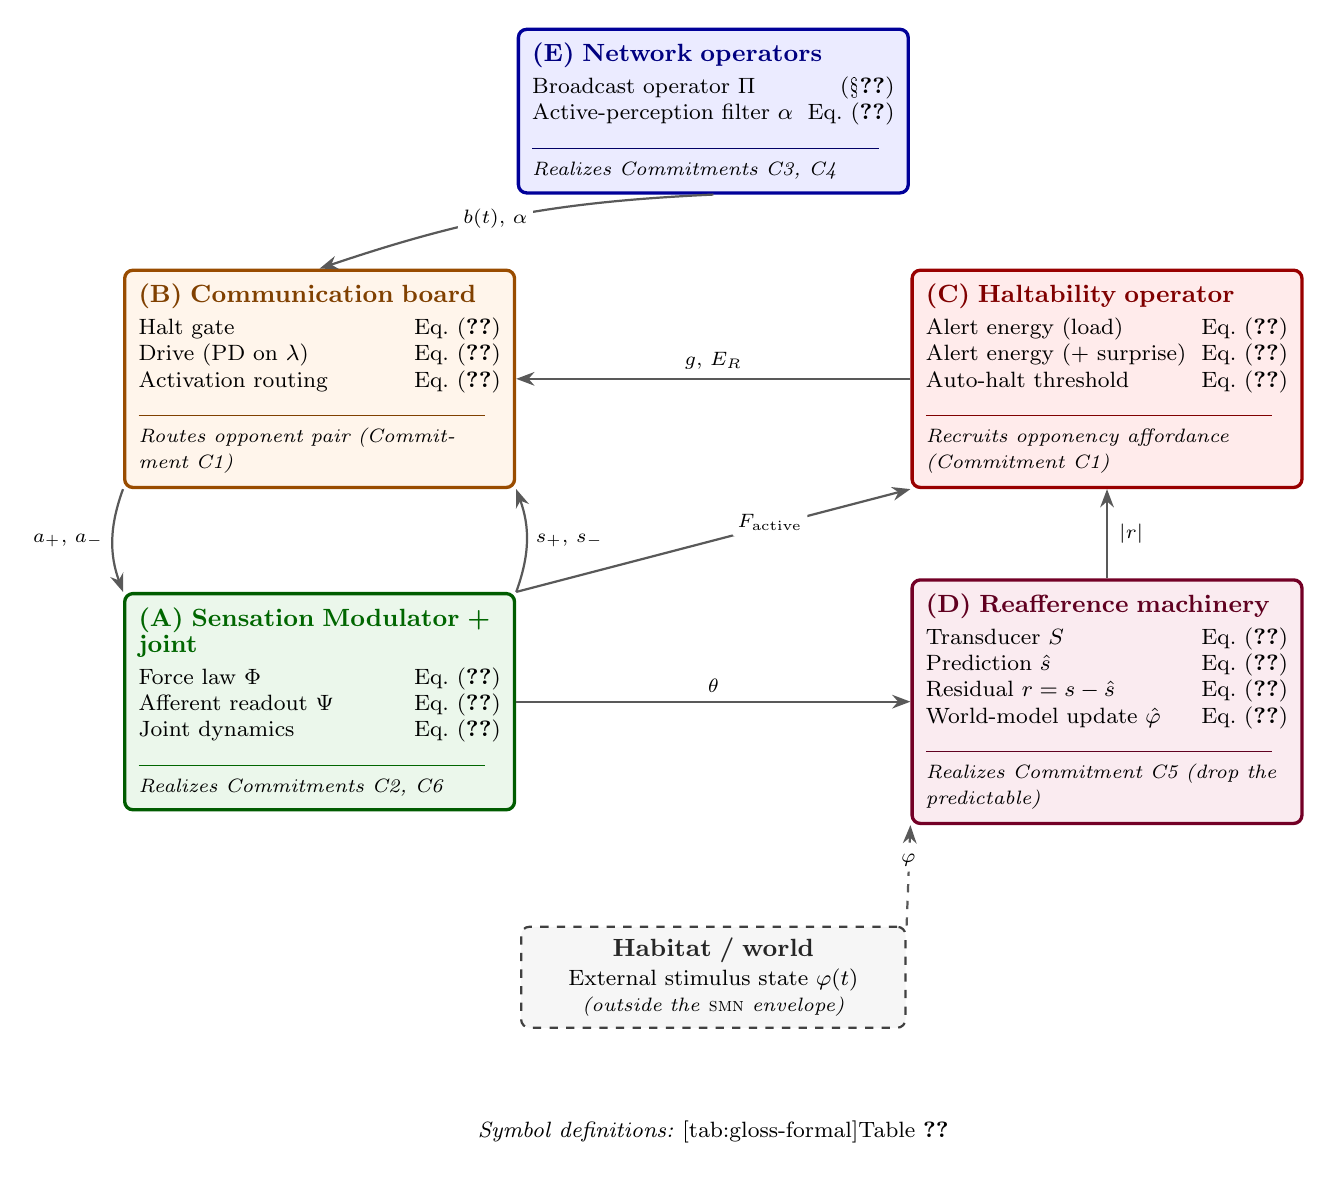
\begin{tikzpicture}[
  cluster/.style 2 args={
    rectangle, rounded corners=3pt, draw=#1!60!black, very thick,
    fill=#1!8, inner sep=5pt, align=left, font=\footnotesize,
    text width=4.6cm
  },
  edge/.style={->, >=Stealth, thick, draw=gray!70!black},
  edgelbl/.style={font=\scriptsize, inner sep=2pt, fill=white,
                  text=black, rounded corners=1pt},
  axiomlbl/.style={font=\scriptsize\itshape, text=gray!40!black}
]

% --- (E) Network operators: top, centered ---
\node[cluster={blue}{}] (net) at (5,5) {%
  {\small\bfseries\color{blue!50!black}(E) Network operators}\\[2pt]
  Broadcast operator $\Pi$ \hfill (\S\ref{sec:smn-tuple})\\
  Active-perception filter $\alpha$ \hfill Eq.~\eqref{eq:alpha-promote}\\[1pt]
  \textcolor{blue!40!black}{\rule{4.4cm}{0.3pt}}\\
  {\scriptsize\itshape Realizes Commitments~C3, C4}
};

% --- (B) Control board: middle-left ---
\node[cluster={orange}{}] (ctrl) at (0,1.6) {%
  {\small\bfseries\color{orange!50!black}(B) Communication board}\\[2pt]
  Halt gate \hfill Eq.~\eqref{eq:halt}\\
  Drive (PD on $\lambda$) \hfill Eq.~\eqref{eq:drive}\\
  Activation routing \hfill Eq.~\eqref{eq:board}\\[1pt]
  \textcolor{orange!50!black}{\rule{4.4cm}{0.3pt}}\\
  {\scriptsize\itshape Routes opponent pair (Commitment~C1)}
};

% --- (C) Haltability operator: middle-right ---
\node[cluster={red}{}] (halt) at (10,1.6) {%
  {\small\bfseries\color{red!50!black}(C) Haltability operator}\\[2pt]
  Alert energy (load) \hfill Eq.~\eqref{eq:alertenergy}\\
  Alert energy (+ surprise) \hfill Eq.~\eqref{eq:alertenergy-with-surprise}\\
  Auto-halt threshold \hfill Eq.~\eqref{eq:autohalt}\\[1pt]
  \textcolor{red!50!black}{\rule{4.4cm}{0.3pt}}\\
  {\scriptsize\itshape Recruits opponency affordance (Commitment~C1)}
};

% --- (A) SM + joint: bottom-left ---
\node[cluster={green!60!black}{}] (mech) at (0,-2.5) {%
  {\small\bfseries\color{green!40!black}(A) Sensation Modulator + joint}\\[2pt]
  Force law $\Phi$ \hfill Eq.~\eqref{eq:Phi}\\
  Afferent readout $\Psi$ \hfill Eq.~\eqref{eq:Psi}\\
  Joint dynamics \hfill Eq.~\eqref{eq:joint}\\[1pt]
  \textcolor{green!40!black}{\rule{4.4cm}{0.3pt}}\\
  {\scriptsize\itshape Realizes Commitments~C2, C6}
};

% --- (D) Reafference machinery: bottom-right ---
\node[cluster={purple}{}] (reaf) at (10,-2.5) {%
  {\small\bfseries\color{purple!50!black}(D) Reafference machinery}\\[2pt]
  Transducer $S$ \hfill Eq.~\eqref{eq:rf}\\
  Prediction $\hat s$ \hfill Eq.~\eqref{eq:s-hat}\\
  Residual $r=s-\hat s$ \hfill Eq.~\eqref{eq:residual}\\
  World-model update $\hat\varphi$ \hfill Eq.~\eqref{eq:phi-update}\\[1pt]
  \textcolor{purple!50!black}{\rule{4.4cm}{0.3pt}}\\
  {\scriptsize\itshape Realizes Commitment~C5 (drop the predictable)}
};

% --- World / habitat node: outside the SMN, centered under E ---
\node[draw=gray!50!black, dashed, thick, rounded corners=3pt,
      fill=gray!7, inner sep=4pt, align=center, font=\footnotesize,
      text width=4.6cm]
  (world) at (5, -6.0) {%
  {\small\bfseries\color{gray!30!black}Habitat / world}\\[1pt]
  External stimulus state $\varphi(t)$\\
  {\scriptsize\itshape (outside the \smn{} envelope)}
};

% --- Edges (variables flowing between sub-systems) ---
\draw[edge] (net.south) to[bend right=8]
  node[edgelbl,pos=0.55] {$b(t),\,\alpha$} (ctrl.north);
\draw[edge] (ctrl.south west) to[bend right=20]
  node[edgelbl,left=1pt] {$a_+,\,a_-$} (mech.north west);
\draw[edge] (mech.north east) to[bend right=20]
  node[edgelbl,right=1pt] {$s_+,\,s_-$} (ctrl.south east);
\draw[edge] (mech.east) -- node[edgelbl,above=1pt] {$\theta$} (reaf.west);
\draw[edge] (mech.north east) -- node[edgelbl,pos=0.55,above right=-1pt]
  {$F_{\rm active}$} (halt.south west);
\draw[edge] (reaf.north) -- node[edgelbl,right=2pt] {$|r|$} (halt.south);
\draw[edge] (halt.west) -- node[edgelbl,above=1pt] {$g,\,E_R$} (ctrl.east);
\draw[edge, dashed] (world.north east) -- node[edgelbl,above=1pt] {$\varphi$}
  (reaf.south west);

\node[font=\footnotesize, anchor=north] at (5, -7.7) {%
  \emph{Symbol definitions:}~%
  \hyperref[tab:gloss-formal]{Table~\ref*{tab:gloss-formal}}%
};

\end{tikzpicture}
\caption{Functional dependency graph of the SMN formalism.  Each
box names a sub-system and lists the equations that live in it;
arrows label the variables that flow between sub-systems.
\textbf{(A)} The Sensation Modulator and the joint produce force
from received activation and emit proprioceptive afferents.
\textbf{(B)} The communication board takes afferents, the broadcast
state, the halt gate and the alert-energy bias, and produces the
two opposing activations.  \textbf{(C)} The haltability operator
integrates motor load and sensory surprise into alert energy and
the halt gate.  \textbf{(D)} The reafference machinery pairs the
agent's proprioception with its world-state estimate to produce
the residual that distinguishes self-generated from
world-generated sensory change.  \textbf{(E)} The network
operators broadcast integrated body state and gate which sensors
enter each board's predictive computation.  Symbols defined in
Table~\ref{tab:gloss-formal}.}
\label{fig:formula-network}
\end{figure}

\begin{table}[h]
\centering
\small
\caption{Formal operators and symbols.}
\label{tab:gloss-formal}
\begin{tabularx}{\linewidth}{@{}l l X l@{}}
\toprule
\textbf{Symbol} & \textbf{Reads} & \textbf{Note} & \textbf{First use} \\
\midrule
$\Phi$ & Force law of an SM. &
$F=\Phi(a,q,\dot q)$, $F\geq 0$ (pull-only); Hill-type in the
reference implementation design.
& Eq.~\eqref{eq:Phi} \\
\addlinespace[2pt]
$\Psi$ & Afferent readout of an SM. &
$s=\Psi(q,\dot q,F)$; identity on $(q,\dot q,F)$ in the reference
implementation design.
& Eq.~\eqref{eq:Psi} \\
\addlinespace[2pt]
$g$ & Halt gate of a CAZ's board. &
$g=1$ permits drive; $g=0$ engages halt. Set by $H$ from
alert-energy and surprise.
& Eq.~\eqref{eq:halt} \\
\addlinespace[2pt]
$\lambda$ & Target equilibrium configuration. &
Set by the agent's task; the joint configuration the board
steers the CAZ toward (Feldman-style equilibrium-point control).
& Eq.~\eqref{eq:drive} \\
\addlinespace[2pt]
$E_R$ & Alert energy. &
Non-negative metabolic cost of maintaining co-activation; built by
load and surprise, decays passively.
& Eq.~\eqref{eq:alertenergy} \\
\addlinespace[2pt]
$\rho,\tau_E,\beta,\gamma$ & Alert-energy parameters. &
Build rate, decay time constant, partner-tonic coupling, post-halt
gain. $\beta$ controls Reg.~1; $\gamma$ controls Reg.~2.
& \S\ref{sec:H} \\
\addlinespace[2pt]
$\rho_r$ & Surprise coupling rate. &
Rate at which $|r|$ builds alert energy; couples reafference to
attention.
& Eq.~\eqref{eq:alertenergy-with-surprise} \\
\addlinespace[2pt]
$\tau_h$ & Surprise threshold for halt. &
Auto-halt engages when $|r(t)|>\tau_h$, with hysteresis on release.
& Eq.~\eqref{eq:autohalt} \\
\addlinespace[2pt]
$r(t)$ & Reafference residual. &
$r=s-\hat s$. Central scalar: nonzero $r$ means the world has done
something the agent's model did not anticipate.
& Eq.~\eqref{eq:residual} \\
\addlinespace[2pt]
$\hat\varphi$ & Predictor's world-state estimate. &
Updated from residual history; used to form $\hat s$.
& \S\ref{sec:transducer} \\
\addlinespace[2pt]
$\hat\psi$ & Predictor's partner-modulation estimate. &
Used in $\mathrm{DSI}^{\mathrm{cross}}$; recoverable because the
partner shares the opponent architecture.
& Eq.~\eqref{eq:dsi-cross} \\
\addlinespace[2pt]
$\kappa$ & World-model learning rate. &
Adaptation rate of $\hat\varphi$ from residual; $\kappa=0$ recovers
the non-learning agent.
& Eq.~\eqref{eq:phi-update} \\
\addlinespace[2pt]
$\Pi$ & Broadcast operator. &
Maps network state to broadcast $b(t)$. Non-degenerate: every CAZ
contributes to and reads from $b$.
& \S\ref{sec:smn-tuple} \\
\addlinespace[2pt]
$\alpha$ & Active-perception filter. &
$\alpha_i(t)\subseteq\mathcal{S}$: sensor streams admitted to CAZ
$i$'s predictive computation. Others remain under peripheral
monitoring.
& \S\ref{sec:smn-tuple} \\
\addlinespace[2pt]
$\mathrm{DSI}^{\mathrm{int}}$ & Internal Dual-Signal Index. &
Reconstruction quality using only SMN-internal broadcast; high in
self-contact.
& Eq.~\eqref{eq:dsi-int} \\
\addlinespace[2pt]
$\mathrm{DSI}^{\mathrm{ext}}$ & External Dual-Signal Index. &
Reconstruction quality given inferred external state $\hat\varphi$;
rises when world dynamics are learnable.
& Eq.~\eqref{eq:dsi-ext} \\
\addlinespace[2pt]
$\mathrm{DSI}^{\mathrm{cross}}$ & Cross-SMN Dual-Signal Index. &
Reconstruction quality given inferred partner state $\hat\psi$;
high in inter-subjective contact.
& Eq.~\eqref{eq:dsi-cross} \\
\bottomrule
\end{tabularx}
\end{table}

\subsection{The Sensation Modulator}\label{app:formal-sm}

The Sensation Modulator described in \S\ref{sec:dpm} of the main
body is specified by two coupled relations:
\begin{align}
F &= \Phi(a,\,q,\,\dot q),
\qquad F\geq 0 \text{ (pull-only)}
\label{eq:Phi}\\
s &= \Psi(q,\,\dot q,\,F).
\label{eq:Psi}
\end{align}
Equation~\eqref{eq:Phi} says that the force the zone produces is a
function of the activation it receives and its current configuration
and velocity, with the pull-only constraint reflecting the
biological fact that muscle (and most analogous tissues) can pull
but not push.  Equation~\eqref{eq:Psi} says that the afferent
signal the zone emits is a function of its configuration, velocity,
and force --- read out by receptors embedded in the same tissue
whose deformation produces $F$.

The defining property is that the same $q$ that determines $F$ via
$\Phi$ also determines $s$ via $\Psi$.  There is no internal
boundary separating ``the sensor'' from ``the actuator''; the
tissue acts and senses through the same substrate.  This is a
substantive empirical claim about muscle--tendon biology,
supported by the literature on muscle spindle, Golgi tendon organ,
and joint receptor placement \citep{ProskeGandevia2012}.

\paragraph*{Structural commitments versus realization.}
The architectural commitments are about the structure of $\Phi$
and $\Psi$, not their parametric form:
\begin{itemize}[itemsep=2pt]
\item $\Phi$ must be pull-only ($F\geq 0$) and depend jointly on
activation $a$ and configuration $(q,\dot q)$.  The architecture
rests on this jointness, because it is what allows the same tissue
to produce force-following-activation in some regimes and
tone-following-load in others.
\item $\Psi$ must report a configuration variable that the next
stage of the SMN can read.  The specific variables (length, force,
velocity, or some combination) and their scaling are
realization-dependent.
\end{itemize}

In our reference implementation $\Phi$ is a Hill-type
force--length--velocity relation and $\Psi$ is essentially the
identity on $(q,\dot q,F)$.  This choice is biologically standard
for vertebrate skeletal muscle and produces realistic
force--length and force--velocity curves.  Other realizations
admit other functional forms: invertebrate muscle, cardiac muscle,
smooth muscle, and various artificial actuators (pneumatic
muscles, dielectric elastomers, McKibben actuators, shape-memory
alloys) all have $(\Phi,\Psi)$ pairs that satisfy the structural
commitments while having different parametric form.  Any
$(\Phi,\Psi)$ satisfying the structural commitments is an
admissible realization of the SM, and the architecture's claims
downstream of \S\ref{sec:dpm} survive substitution.

The descriptive treatment of the Sensation Modulator, including
the realization-independence point and the controller--plant
decomposition violation, is in \S\ref{sec:dpm} of the main body.

\subsection{The Coordinated Action Zone}\label{app:formal-caz}

The CAZ described in \S\S\ref{sec:caz}--\ref{sec:H} of the main
body is the tuple $(Z_+, Z_-, B, H)$ with state variables
$(q,\dot q)$ for the shared configuration and an internal state
$E_R$ for the haltability operator.  This subsection states the
joint dynamics, the routing law of the board, and the dynamics of
the haltability operator.

\paragraph*{Joint dynamics.}
For a one-degree-of-freedom joint with moment arm $r$ and inertia
$I$,
\begin{equation}
I\,\ddot q = r\,(F_+ - F_-) - b\,\dot q,
\label{eq:joint}
\end{equation}
where $F_\pm = \Phi(a_\pm,\ell_\pm,\dot\ell_\pm)$ with
$\ell_+ = \ell_0 - r q$ and $\ell_- = \ell_0 + r q$.  Equation
\eqref{eq:joint} is standard; what is non-standard is that $a_+$
and $a_-$ are not independent commands from a controller but
emerge from the board's routing specified below.

\paragraph*{The communication board.}
The board implements three functions: it reads the proprioceptive
signal each zone emits, it applies a halt gate $g\in\{0,1\}$, and
it emits the reciprocal activation each zone receives subject to
alert-energy modulation.  Throughout this paper, $g=1$ denotes
``active drive permitted'' and $g=0$ denotes ``halt engaged'':
\begin{equation}
\text{If } g=0\,(\text{halt}):\quad a_+ = a_- = a_0,
\label{eq:halt}
\end{equation}
\begin{equation}
\text{If } g=1\,(\text{active}):\quad
\text{drive} = K_p(\lambda - q) - K_d\,\dot q,
\label{eq:drive}
\end{equation}
\begin{equation}
\begin{aligned}
&\text{drive}\geq 0:
&\;a_+ &= \mathrm{clip}(\text{drive},0,1),
&\;a_- &= \mathrm{clip}(a_0 + \beta E_R,0,1),\\
&\text{drive}<0:
&\;a_- &= \mathrm{clip}\bigl(-\text{drive}\cdot(1+\gamma E_R),0,1\bigr),
&\;a_+ &= \mathrm{clip}(a_0 + \beta E_R,0,1).
\end{aligned}
\label{eq:board}
\end{equation}
Here $a_0 > 0$ is the baseline co-contraction (the alert tonic
activity of the inactive zone), $\lambda$ is the equilibrium
configuration set by the agent's task, and $(\beta,\gamma)$ are
the coupling coefficients of the haltability operator.

The second branch of \eqref{eq:board} formalizes an asymmetry
essential to the architecture: when one zone is active, the other
contributes baseline $a_0$ plus an alert-energy bias $\beta E_R$;
when the active zone changes (the drive flips sign), the
previously alert zone's drive is amplified by $(1+\gamma E_R)$,
giving it a head start in taking over.

\phantomsection\label{app:formal-H}
\paragraph*{The haltability operator.}
The state variable of $H$ is the \emph{alert energy} $E_R\geq 0$:
\begin{equation}
\boxed{\;
\frac{dE_R}{dt} = \rho\,F_{\text{active}}\,\mathbf{1}[g=1]
              - \frac{E_R}{\tau_E}.
\;}
\label{eq:alertenergy}
\end{equation}
$F_{\text{active}} = \max(F_+, F_-)$ is the force generated by
whichever zone is currently active, $\rho$ is the build rate,
$\tau_E$ is the decay time constant, and $\mathbf{1}[g=1]$ is the
indicator function for ``not halted.''  Alert energy accumulates
while the system is actively driving a zone, in proportion to the
load that zone carries; it decays passively when not being
driven.

The steady state when the active zone is loaded with average
force $\langle F_{\text{active}}\rangle$ is
\begin{equation}
E_R^* = \rho\,\tau_E\,\langle F_{\text{active}}\rangle.
\label{eq:Estar}
\end{equation}
This is the load-scaled active equilibrium described in
\S\ref{sec:H} of the main body.

The descriptive treatment of the CAZ --- its three structural
properties, the architectural role of antagonism, the affordance
analysis of haltability, and the three architectural consequences
of alert energy --- is in \S\S\ref{sec:caz}--\ref{sec:H} of the
main body.

\subsection{Transducers and the reafference principle}\label{app:formal-reaf}

The transducer described in \S\ref{sec:transducer-defn} of the
main body converts a physical perturbation in the agent's
environment into a neural signal:
\begin{equation}
S : \Phi(t,x) \mapsto s(t),
\label{eq:transducer-map}
\end{equation}
where $\Phi(t,x)$ is the relevant physical field (light
intensity, sound pressure, chemical concentration, mechanical
contact) and $s(t)$ is a train of action potentials or its rate
equivalent.  The transducer is read-only: unlike the Sensation
Modulator (\S\ref{app:formal-sm}), it does not write back into
the mechanical state of the body.

For a one-degree-of-freedom agent with joint angle $\theta$ and a
stimulus at angular position $\varphi$, the simplest non-trivial
form is a Gaussian receptive field:
\begin{equation}
s(t) = I \exp\!\left(- \frac{(\theta(t) - \varphi(t))^2}{\sigma^2}
\right) + \eta(t),
\label{eq:rf}
\end{equation}
with $I$ the stimulus intensity, $\sigma$ the receptive-field
width, and $\eta$ small additive sensory noise.  Other tuning
forms (orientation columns, place fields, chemoreceptor
concentration curves) are admissible substitutes; the structural
commitment is that $s$ depends jointly on $\theta$ (the agent's
configuration, modulable by action) and $\varphi$ (the world,
only conditionally observable).

\paragraph*{The reafference predictor.}
A \emph{reafference predictor} is added as a sub-component of the
communication board.  It receives the proprioceptive estimate of
$\theta$ delivered veridically by the CAZ's modulators, and the
agent's internal estimate $\hat\varphi$ of the world state.  It
produces a predicted sensor reading
\begin{equation}
\hat s(t) = I \exp\!\left(- \frac{(\theta(t) - \hat\varphi(t))^2}{\sigma^2}\right),
\label{eq:s-hat}
\end{equation}
and the architecture's central scalar quantity, the
\emph{reafference residual}:
\begin{equation}
r(t) = s(t) - \hat s(t).
\label{eq:residual}
\end{equation}
The predictor uses the actual $\theta$, not a prediction of it,
because the agent's own configuration is directly observable
through the Sensation Modulators of its CAZs.  What the agent
cannot directly observe is the world: it has only an estimate,
updated from history.

\paragraph*{Coupling residual to alert energy.}
The alert-energy dynamics of \S\ref{app:formal-H} are extended so
that the surprise signal $|r|$ also builds $E_R$:
\begin{equation}
\boxed{\;
\frac{dE_R}{dt} = \rho\,F_{\text{active}}\,\mathbf{1}[g=1]
              + \rho_r\,|r(t)|
              - \frac{E_R}{\tau_E}.
\;}
\label{eq:alertenergy-with-surprise}
\end{equation}
Two sources now build alert energy: the load on the active zone
(as before), and the magnitude of the reafference residual.

The auto-halt condition is
\begin{equation}
g(t+) = 0 \;\Longleftrightarrow\; |r(t)| > \tau_h
\quad\text{(with hysteresis on release)},
\label{eq:autohalt}
\end{equation}
where $\tau_h$ is the surprise threshold for halt initiation.  In
the implementation design, halt persists until $|r| < \tau_h/2$,
which prevents chattering at threshold.

\paragraph*{World-model adaptation.}
Sensorimotor contingency mastery requires the world model to
adapt.  We use a gradient-style update of $\hat\varphi$ from the
residual:
\begin{equation}
\frac{d\hat\varphi}{dt} = \kappa\,\frac{r(t)}{\partial \hat s/\partial \varphi},
\label{eq:phi-update}
\end{equation}
clipped to bound the step size, with $\kappa$ a learning rate.
Equation~\eqref{eq:phi-update} is a Newton-like step on the
world state given the receptive-field structure: where the
receptive field is informative about $\varphi$ (gradient
$\partial\hat s/\partial\varphi\neq 0$), the residual carries
usable information; where the receptive field is flat, the
residual is uninformative and no update occurs.  Mastery of a
sensorimotor contingency is quantified as the rate of decay of
$|r(t)|$ following a world change.

\paragraph*{The dual-signal structure.}
The multi-CAZ body's default mode is a SMAP-running body
(\S\ref{sec:smap} of the main body).  Let
$y_t\in\mathbb{R}^m$ be the concatenated afferent vector across
all the body's transducers and proprioceptors, and let
$\boldsymbol\theta_t = (\theta_1, \theta_2, \dots)$ be the joint
configuration vector of all CAZs.  Define the modulation map
\begin{equation}
F(\boldsymbol\theta_t;\,z_t):\Theta\to\mathbb{R}^m,
\qquad
y_t = F(\boldsymbol\theta_t;\,z_t),
\label{eq:F-modulation}
\end{equation}
where $z_t$ is the background state held fixed (BAPs running,
gravitational context, etc.).  Equation~\eqref{eq:F-modulation}
is the body's own forward-kinematics-and-mechanics relation: it
tells how modulation of any $\theta_i$ changes the sensed
feedback of every transducer that depends on the body's
configuration.

A SMAP is a coordinated trajectory of activations
$\pi = \langle a_t \rangle_{t=1}^T$ for which:
\begin{description}[itemsep=2pt,labelindent=0pt,leftmargin=4em,
                    style=nextline]
\item[(SMAP-1)]
There exists at least one endogenous sensor $s$ with nonzero
agent-controlled sensitivity to the modulation parameter:
$\partial F_s / \partial \theta_t > 0$.
\item[(SMAP-2)]
The pattern is agent-haltable: the haltability operator
(\S\ref{app:formal-H}) can gate the modulation.
\end{description}

A SMAP is \emph{dual-signal} if there exist two CAZs $Z_x, Z_y$
in the SMN graph, with respective efferent activations $a_x, a_y$
and afferent streams $s_x, s_y$, such that:
\begin{description}[itemsep=2pt,labelindent=0pt,leftmargin=4em,
                    style=nextline]
\item[(DS-1) Shared sensitivity]
$s_x$ and $s_y$ are both sensitive to a common modulation
parameter $\theta$:
$\partial F_{s_x}/\partial \theta > 0$ and
$\partial F_{s_y}/\partial \theta > 0$.
\item[(DS-2) Both efference copies in broadcast]
Both efferent activations $a_x$ and $a_y$ are available to the
predictor through the SMN's broadcast operator $\Pi$:
$a_x, a_y \subseteq b(t)$ at every $t$ during the trajectory.
\item[(DS-3) Haltability]
The pattern is agent-haltable through the haltability operator
$H$.
\item[(DS-4) Trajectory closure within the SMN graph]
The coupled trajectory $(s_x(t), s_y(t), a_x(t), a_y(t))$
remains within the SMN-internal portion of the message graph for
the duration of $\pi$.  No part of the modulation passes through
a transducer reading an external state, and no component of
$a_x$ or $a_y$ is computed from external state estimation.
\end{description}

The strengthening matters.  Shared sensitivity (DS-1) alone is
too weak: two externally coupled sensors could also be sensitive
to the same environmental parameter, satisfying (DS-1) without
being SMAP-coupled.  (DS-2) and (DS-4) supply the architectural
content that the weaker condition does not.  With all four
conditions, dual-signal-positive trajectories are architecturally
identifiable, not merely correlationally similar to within-body
coupling.

\paragraph*{The Dual-Signal Index (three forms).}
The architectural distinction between SMAP-coupled, externally
coupled, and inter-subjectively coupled streams admits a
quantitative metric in three contrasting forms.

The \emph{internal} index measures how well the predictor's
reconstruction of $s_y$ tracks the actual sensor when the
predictor is constrained to use only SMN-internal broadcast
variables:
\begin{equation}
\mathrm{DSI}^{\mathrm{int}}_{xy}(t) = \mathrm{corr}\!\left(\,
s_y(t),\;
\hat s_y\!\left(t\,\bigm|\,
\theta_x(t),\theta_y(t),a_x(t),a_y(t)\right)\,\right),
\label{eq:dsi-int}
\end{equation}
where the conditioning variables in the predictor's input are
all elements of $b(t) = \Pi(\mathbf{X}(t))$ --- they live inside
the SMN's broadcast and are therefore architecturally available
without requiring estimation of any external state.

The \emph{external} index measures the same reconstruction when
the predictor uses an inferred external-state variable
$\hat\phi(t)$:
\begin{equation}
\mathrm{DSI}^{\mathrm{ext}}_{xy}(t) = \mathrm{corr}\!\left(\,
s_y(t),\;
\hat s_y\!\left(t\,\bigm|\,
\theta_x(t),\hat\phi(t)\right)\,\right),
\label{eq:dsi-ext}
\end{equation}
where $\hat\phi(t)$ is the predictor's running estimate of an
external object's state, computed from the afferent history.

The \emph{cross-SMN} index measures partner-specific structured
coupling recoverable when the predictor uses an inferred
partner-state estimate $\hat\psi(t)$, constrained to track
intentional structure in the afferent stream rather than the
unstructured dynamics that $\hat\phi$ accommodates:
\begin{equation}
\mathrm{DSI}^{\mathrm{cross}}_{xy}(t) = \mathrm{corr}\!\left(\,
s_y(t),\;
\hat s_y\!\left(t\,\bigm|\,
\theta_x(t),\hat\psi(t)\right)\,\right).
\label{eq:dsi-cross}
\end{equation}

Together the three indices give the architectural geometry of
contact: high $\mathrm{DSI}^{\mathrm{int}}$ marks self-contact
(the second efferent partner is in the agent's own broadcast);
rising $\mathrm{DSI}^{\mathrm{ext}}$ marks learnable
world-contact (a non-SMN object whose dynamics can be learned
through external-state estimation); high
$\mathrm{DSI}^{\mathrm{cross}}$ marks inter-subjective contact
(another SMN whose structured modulation can be partially
recovered from the contact's structure but not from the agent's
own internal broadcast).

The descriptive treatment of transducers, the reafference
principle, the predictor, sensorimotor contingencies, SMAPs, the
dual-signal property, the three configurations of contact, and
the shared-intentionality hypothesis is in
\S\S\ref{sec:transducer}--\ref{sec:shared} of the main body.

\subsection{The phase-oscillator description (multi-CAZ chains)}\label{app:formal-osc}

The continuous dynamical-systems picture of a multi-CAZ system
described in \S\ref{sec:bridge} of the main body uses
Kuramoto-style coupled oscillators with interrupts.

For a chain of $N$ segmental CAZs each driven by a central
pattern generator with intrinsic frequency $\omega_i$ and phase
$\theta_i$, with nearest-neighbour coupling $K_{ij}$ and target
phase lag $\varphi_{ij}$, the framework adopts the standard form
\begin{equation}
\dot\theta_i = \omega_i + \sum_{j\in\mathcal N(i)}
K_{ij}\sin(\theta_j - \theta_i - \varphi_{ij}) + u_i(t),
\label{eq:kuramoto}
\end{equation}
where $u_i(t)$ is the modulatory input from the SMN.

The modulatory input is the haltability-gated drive emitted by
the $i$th CAZ's communication board (\S\ref{app:formal-caz}),
reflecting both the local affordance signal and the broadcast
state of the network.  This identification is what converts
\eqref{eq:kuramoto} from an illustrative gesture into a
specification: $u_i$ is computed by the architecture
(specifically, by the haltability operator of
\S\ref{app:formal-H} applied to the local CAZ), not stipulated.

\paragraph*{The four regimes formally.}
\textbf{BAP (Basal Action Pattern).}  $u_i \equiv 0$; the chain
runs purely on $(\omega_i, K_{ij}, \varphi_{ij})$.  Stable
limit-cycle oscillation.

\textbf{HAP (Haltable Action Pattern).}  $u_i$ is a phase-reset
pulse that gates $\theta_i$ to a halt value with the halt
operator of \S\ref{app:formal-H} active.
Equation~\eqref{eq:alertenergy} governs $E_R$ during the halt.

\textbf{NAP (Negotiable Action Pattern).}  $u_i$ continuously
rephases or reweights $K_{ij}$ in response to perceptual
predicates (\S\ref{app:formal-network}).

\textbf{TAP (Transactional Action Pattern).}  NAPs whose
phase-reset events are externalized --- the halt pulse leaves a
public trace recoverable by other agents.  This is a property of
the agent--environment--other coupling, not of
\eqref{eq:kuramoto} alone.

The descriptive treatment of the four regimes, their
architectural significance, and what the phase-oscillator
description adds beyond single-CAZ dynamics is in
\S\ref{sec:bridge} of the main body.

\subsection{Multi-CAZ networks: the SMN as a hybrid graph-dynamical system}\label{app:formal-network}

The SMN of \S\ref{sec:network} of the main body is specified as
a tuple
\begin{equation}
\mathrm{SMN}=(G,\mathcal{Z},\mathcal{B},\mathcal{H},\mathcal{S},
              \Pi,\alpha)
\label{eq:smn-tuple}
\end{equation}
whose components fall into three groups: a routing graph $G$
over CAZ nodes $\mathcal{Z}$, the local-dynamical operators
$\mathcal{B}$ (boards) and $\mathcal{H}$ (haltability) attached
to each node, and the network-level operators $\Pi$ (broadcast)
and $\alpha$ (active-perception filter) acting over the sensor
space $\mathcal{S}$.  Table~\ref{tab:smn-tuple} gives each
component's type and architectural role.

\begin{table}[h]
\centering
\small
\caption{Components of the SMN tuple of equation~\eqref{eq:smn-tuple}.}
\label{tab:smn-tuple}
\begin{tabularx}{\linewidth}{@{}l l X@{}}
\toprule
\textbf{Component} & \textbf{Reads} & \textbf{Note} \\
\midrule
$G=(V,E)$ & Routing graph. &
$V$ finite set of CAZ nodes; $E\subseteq V\times V$ directed
routing edges. Edges encode the architectural possibility of
message flow; actual flow depends on $\Pi$ and $\alpha$. \\
\addlinespace[2pt]
$\mathcal{Z}=\{C_i\}_{i\in V}$ & CAZ nodes. &
Each $C_i=(Z_i^+,Z_i^-,B_i,H_i)$ as in \S\ref{app:formal-caz}. \\
\addlinespace[2pt]
$\mathcal{B}=\{B_i\}_{i\in V}$ & Local boards. &
$B_i:(s_i^+,s_i^-,b(t),\lambda_i,g_i,E_R^i,\alpha_i(t)) \mapsto
(a_i^+,a_i^-)$. \\
\addlinespace[2pt]
$\mathcal{H}=\{H_i\}_{i\in V}$ & Haltability operators. &
Each $H_i$ acts on $C_i$ as in \S\ref{app:formal-H}, with state
$E_R^i$ evolving by equation~\eqref{eq:alertenergy}. \\
\addlinespace[2pt]
$\mathcal{S}$ & Sensor space. &
All transducers in the SMN, distributed across CAZs and at the
body--habitat boundary. \\
\addlinespace[2pt]
$\Pi:\mathbf{X}(t)\mapsto b(t)$ & Broadcast operator. &
Maps the full network state $\mathbf{X}(t)=(x_1,\ldots,x_N)$
with $x_i=(q_i,\dot q_i,a_i^+,a_i^-,s_i^+,s_i^-,E_R^i,g_i)$ to
$b(t)\in\mathbb{R}^d$ available to every board. Architectural
commitment: \emph{non-degeneracy} (every CAZ contributes to and
reads from $b$). \\
\addlinespace[2pt]
$\alpha=\{\alpha_i(t)\}_{i\in V}$ & Active-perception filter. &
$\alpha_i(t)\subseteq\mathcal{S}$: sensor streams admitted to
$B_i$'s predictive computation at time $t$. Realizes Commitment~C4. \\
\bottomrule
\end{tabularx}
\end{table}

\paragraph*{Network closure.}
The architectural commitment on $\Pi$ is non-degeneracy: every
CAZ contributes to and reads from $b(t)$.  The condition is
graph- and operator-theoretic and can be checked on a candidate
implementation.

\paragraph*{Two-stage gating: the active-perception filter promotion rule.}
A stream $S_j$ is promoted into $\alpha_i(t+\Delta t)$ when
\begin{equation}
\mathrm{corr}(\Delta s_j, a_i) > \epsilon
\quad\text{or}\quad
|\Delta s_j| > \tau_s,
\label{eq:alpha-promote}
\end{equation}
i.e.\ when the stream has begun coupling to action ($\epsilon$)
or has changed enough to be unsafe to ignore regardless of
coupling ($\tau_s$).  Equation~\eqref{eq:alpha-promote} is the
working specification of Commitment~C4; the exact functional form,
the timescale $\Delta t$, the rule for demotion, and the cost
structure of peripheral monitoring are open for refinement.

\paragraph*{Network dynamics.}
Each CAZ $i$ evolves as
\begin{equation}
\dot x_i = f_i\!\left(x_i,\ b(t),\ \{s_j\}_{j\in\alpha_i(t)},
                       \lambda_i\right),\qquad
b(t) = \Pi(\mathbf{X}(t)),
\label{eq:network-dyn}
\end{equation}
where $f_i$ is the single-CAZ dynamics of \S\ref{app:formal-caz}
(joint dynamics, board, haltability), parameterized by the
broadcast state and the attended sensor streams.
Equation~\eqref{eq:network-dyn} is a coupled
differential-equation system on a graph; its analytical
treatment for arbitrary network topologies is deferred
(\S\ref{app:formalism-kind}).

\paragraph*{Anatomical regimes as parameter patterns.}
The local board $B_i$ at the $i$th CAZ receives, in addition to
its own $(s_+^i, s_-^i)$, two further inputs: the BAP backdrop
$\mathbf{f}(t)$ (a low-dimensional projection of the phases of
the continuously running CAZs) and the broadcast state $b(t)$.
The drive equation~\eqref{eq:drive} generalizes to
\begin{equation}
\text{drive}_i = K_p^i(\lambda_i - q_i) - K_d^i\dot q_i
              + W_f^i\,\mathbf{f}(t) + W_x^i\,b(t),
\label{eq:network-drive}
\end{equation}
where $W_f^i$ and $W_x^i$ are routing weights that determine
how the $i$th CAZ is influenced by the BAP backdrop and the
broadcast state.  Different anatomical regimes correspond to
different patterns of $(W_f^i, W_x^i)$:

\begin{description}[itemsep=2pt,labelindent=0pt,leftmargin=4em,
                    style=nextline]
\item[Synchronous-bilateral coupling (axial locomotion)]
left and right axial CAZs share strong $W_f^i$ from a common
gait BAP; the broadcast contribution $W_x^i$ is small.
\item[Decoupled-appendicular operation (manipulation)]
limb CAZs have $W_f^i \approx 0$ (transiently uncoupled from the
gait backdrop) and large $W_x^i$ (driven by current task state).
\item[Postural--manipulatory integration]
both $W_f^i$ and $W_x^i$ are non-trivial: the trunk maintains
gait-like stability while the hand performs a halted,
negotiated action.
\end{description}

The descriptive treatment of the SMN as a hybrid
graph-dynamical system, network closure, two-stage gating, what
kind of network the SMN is (and is not), and why the layered
network is required are in \S\ref{sec:network} of the main body.

\subsection{Predicted registers}\label{sec:registers}

The formalism produces eight predicted registers, of which seven
are empirically testable and one is explicitly hypothetical:
two from the bare CAZ (\S\ref{sec:caz}); three from the addition of
transducers and reafference (\S\ref{sec:transducer});
one from the integration of haltability and reafference through
alert energy; one structural register of intra-body SMAPs
(\S\ref{sec:smap}); a hypothesis about shared intentionality as
inter-body extension (\S\ref{sec:shared}); and one summary
register of the dual-signal contrast across the three structural
configurations of \S\ref{sec:smap}. Numerical results in the
accompanying simulation figures (\S\ref{app:simulations}).

\begin{description}[itemsep=4pt,labelindent=0pt,leftmargin=2em,
                    style=nextline]
\item[Register 1 (tonic load coupling):]
During steady-state engagement of one zone, the partner zone's tonic
activation $a_{\text{partner}}$ is monotonically increasing in the
active zone's force $F_{\text{active}}$. From \eqref{eq:Estar} and
the steady-state version of \eqref{eq:board},
\begin{equation}
a_{\text{partner}} \approx a_0 + \beta\rho\tau_E
F_{\text{active}},
\label{eq:sig1}
\end{equation}
linear in load with slope $\beta\rho\tau_E$. Classical inhibition
predicts $a_{\text{partner}}=a_0$ independently of load.

\item[Register 2 (resumption latency):]
After a short halt during active engagement, the latency to reach a
small reversed target is shorter under SMN than under classical
inhibition, with the magnitude of the advantage
\begin{equation}
\Delta t \approx \frac{\gamma E_R(t_{\text{release}})}{K_p},
\label{eq:sig2}
\end{equation}
controlled by the gain $\gamma$ and the alert energy at the moment of
halt release.

\item[Register 3 (reafference --- self versus world):]
For a fixed change in the sensor reading, the residual $|r(t)|$ is
small when the change is self-generated (agent moves through a static
world, predictor tracks) and large when the change is world-generated
(agent still while world moves, $\hat\varphi$ outdated). The ratio is
bounded only by sensor noise: in the limit of perfect proprioception
and zero noise, the self-residual is identically zero. This realizes
the \emph{Reafferenzprinzip}
\citep{vonHolstMittelstaedt1950,CrapseSommer2008} as a quantitative
signature.

\item[Register 4 (sensorimotor contingency mastery):]
With $\kappa > 0$ in equation~\eqref{eq:phi-update}, the residual
following a world change decays at a rate determined by the learning
rate and the receptive-field gradient. Mastery is measurable as the
rolling-RMS residual approaching the noise floor following each
world-state change. This realizes the O'Regan--No{\"e} theory of
perception as mastery of sensorimotor contingencies
\citep{OReganNoe2001Sensorimotor} as a measurable adaptation process.

\item[Register 5 (intra-body SMAP / dual-signal residual):]
For any two CAZs of the same SMN whose mechanical states co-determine
a shared sensory substrate, the partner CAZ's $\theta$ is available
to the predictor through cross-zone broadcast, and the residual stays
at the sensor noise floor without any world-model adaptation.
Equivalently, when the residual is regressed against the
partner-as-stimulus form
\begin{equation}
\Delta\hat s(\theta_1,\theta_2,\hat\varphi_2)
= I\!\left[\exp\!\left(-\tfrac{(\theta_2-\theta_1)^2}{\sigma^2}\right)
        - \exp\!\left(-\tfrac{(\theta_2-\hat\varphi_2)^2}{\sigma^2}\right)\right],
\label{eq:sig5}
\end{equation}
where $I$ is the receptive-field intensity from
equation~\eqref{eq:rf} and the second term is the prediction the
predictor would make under the cold-start estimate
$\hat\varphi_2$, $R^2 \to 1$. For a decoupled control in which the
same agent's transducer reads an exogenous stimulus unrelated to
the partner CAZ, the same regression yields $R^2 \to 0$. The
signature is therefore a \emph{structural} feature of the residual,
not a magnitude difference, which makes it diagnostic and not
confounded by overall noise level. This is the empirical
realization of the dual-signal property (DS-1)--(DS-4).

\item[Register 6 (surprise-driven attention and auto-halt):]
With the surprise term in
equation~\eqref{eq:alertenergy-with-surprise} active, an unpredicted
sensory event during ongoing action drives $|r|$ above the threshold
$\tau_h$ of equation~\eqref{eq:autohalt}, which gates the active drive
within one integration step. The same alert-energy substrate that
distinguishes haltability from inhibition is therefore also the
substrate of attention: the architecture unifies the two phenomena
under a single dynamics. This is the empirical signature of cognitive
inertia being disrupted by an affordance change in the sense
made precise in \S\ref{sec:transducer}.

\item[Register 7 (shared intentionality, hypothesis):]
Two SMN agents engaged in mutual reafference (case (c) of
\S\ref{sec:smap}, with both predictors adapting via
equation~\eqref{eq:phi-update}) show a joint mutual residual
$\sqrt{r_1^2 + r_2^2}$ that decays toward the sensor noise floor.
With both agents adapting at non-zero $\kappa$, the late-phase mutual
residual is dramatically reduced relative to (i)~asymmetric adaptation
(only one participant adapting) and (ii)~no adaptation
(reduction $\sim 92\%$ vs.\ neither-adapts in the reference
simulation). We hypothesize that the decay rate of the joint
mutual residual is the empirical signature of shared intentionality
in the sense of \citet{Tomasello2005Understanding}: two predicting
agents converging on a coordinated representation of each other's
actions, mediated by the same reafference machinery that underwrites
intra-body SMAPs (\S\ref{sec:smap}).

\item[Register 8 (the dual-signal contrast: self / world / other):]
Register~8 is a \emph{unifying re-presentation} of the contrast
already exhibited piecewise by Register~5 (the self-contact /
intra-body case), Register~7 (the inter-subjective case under mutual
adaptation), and the world-contact configuration. We list it
separately because the three configurations together expose a
three-dimensional architectural contrast that none of the
component registers exhibits alone, not because it is an
independent empirical prediction. The three Dual-Signal Indices
defined in \S\ref{app:formal-reaf} ---
$\mathrm{DSI}^{\mathrm{int}}$,
$\mathrm{DSI}^{\mathrm{ext}}$,
$\mathrm{DSI}^{\mathrm{cross}}$
--- give the architectural geometry of contact:
self-contact (case (a), partner CAZ in the same SMN with broadcast
access) drives $\mathrm{DSI}^{\mathrm{int}}\to 1$ once the broadcast
operator $\Pi$ has settled, without residual-driven adaptation;
world-contact (case (b), no SMN-internal partner of any kind)
gives $\mathrm{DSI}^{\mathrm{int}}\to 0$ and
$\mathrm{DSI}^{\mathrm{cross}}\to 0$, with $\mathrm{DSI}^{\mathrm{ext}}$
rising if and only if the external dynamics are learnable;
inter-subjective contact (case (c), partner CAZ in another SMN)
gives low $\mathrm{DSI}^{\mathrm{int}}$ but
$\mathrm{DSI}^{\mathrm{cross}}$ rising with adaptation toward
intermediate-to-high values. This is the architectural fact that
the SMN admits a three-way structural distinction between contact
that is broadcast-internal, contact with a non-intentional
exterior, and contact with another agent's structured modulation.
We claim that the distinction is \emph{architecturally available}
on this account, not that the agent thereby \emph{has} self,
world, and other in any developmentally rich sense; how the
agent comes to detect and use this distinction is the work of
the companion program (\S\ref{sec:roadmap}, items~1--2).
\end{description}

\paragraph{Consequences awaiting implementation.}
The network-level formalism of \S\ref{sec:network} entails three
further predictions that the present reference simulation does
not exercise --- they are consequences of the architecture rather
than additional registers, and their precise quantification
requires a multi-CAZ implementation:
\begin{enumerate}[leftmargin=2em,itemsep=2pt]
\item \textbf{BAP-backdrop entrainment.} \hap-level \caz{}s should
exhibit phase-locked modulation by ongoing BAPs with a strength
predicted by the routing weight $W_f^i$.
\item \textbf{Mode-switching latency between axial and appendicular
regimes.} The transition between bilateral coupling and decoupled
appendicular operation should exhibit a characteristic switching
signature at the network level (analogous to phase transitions in
the Haken--Kelso--Bunz (HKB) bimanual coordination model
\citep{HakenKelsoBunz1985PhaseTransitions}).
\item \textbf{Hebbian recruitment of \nap{}s.} Recurrently co-active
\caz{}s should develop strengthened cross-routing weights at the
broadcast level.
\end{enumerate}
We do not number these as Registers 9--11 because they presuppose
an implementation the present preprint does not provide; they are
flagged here so that downstream multi-CAZ implementations can
recognize them as targets.

\subsection{Results of simulations}\label{app:simulations}

The reference simulations realize the architectural specification
in code and demonstrate that the equations generate the predicted
contrasts.  This subsection reports the simulation outputs that
correspond to the CAZ architecture (\S\S\ref{sec:caz}--\ref{sec:H}
in the main body); simulations relating to reafference,
sensorimotor contingencies, intra-body coordination, attention,
and shared intentionality will be added as the corresponding
main-body sections are populated.

\paragraph*{Reach-halt-reverse, CAZ versus classical inhibition.}
Figure~\ref{fig:traces} compares an SMN CAZ against a
classical-inhibition control through a reach-halt-reverse
protocol.  Alert energy $E_R(t)$ builds during reach, decays
during halt, and rebuilds during reverse reach in the SMN; under
classical inhibition $E_R\equiv 0$ throughout.  The two
architectures produce nearly identical trajectories on this
intermediate-amplitude protocol; the architectural difference
shows in the activation/force traces and in the alert-energy
panel.

\begin{figure}[!htbp]
\centering
\includegraphics[width=0.86\linewidth]{fig1_traces.pdf}
\caption{Trace comparison of an SMN CAZ (solid blue) against a
classical-inhibition CAZ (dashed red) in a reach-halt-reverse
protocol. From top to bottom: joint angle $\theta(t)$; activations
of flexor and extensor zones; forces; alert energy $E_R(t)$. The
shaded band marks the halt interval.}
\label{fig:traces}
\end{figure}

\paragraph*{Register~1 --- tonic load coupling.}
The partner zone's steady-state tonic activation scales linearly
with the active zone's force under SMN haltability and is flat
under classical inhibition (Figure~\ref{fig:sig1}).  The slope
is identifiable from this signature alone and is governed by
$\beta\rho\tau_E$.

\begin{figure}[!htbp]
\centering
\begin{subfigure}[c]{0.30\linewidth}
  \centering
  \includegraphics[width=\linewidth]{sketch_R1_tonic_load.png}
  \caption*{}
\end{subfigure}\hfill
\begin{subfigure}[c]{0.66\linewidth}
  \centering
  \includegraphics[width=\linewidth]{fig2_signature1.pdf}
  \caption*{}
\end{subfigure}
\caption{Register~1: tonic load coupling. \emph{Left}: an agent
holds a load with one outstretched arm; the active zone (deltoid,
filled triangle) drives the load while the unloaded arm's deltoid
sits at a tonic engagement that scales with the load. \emph{Right}:
the partner zone's steady-state tonic activation scales linearly
with the active zone's force under SMN haltability (slope $\approx
\beta\rho\tau_E$), and is flat under classical inhibition. The
slope is independent of the gain coefficient $\gamma$, so
$\beta\rho\tau_E$ is identifiable from this signature alone.}
\label{fig:sig1}
\end{figure}

\paragraph*{Register~2 --- post-halt resumption latency.}
Latency to threshold-crossing after halt release, as a function
of halt duration, shows a constant offset between SMN and
classical inhibition rather than a duration-dependent gap
(Figure~\ref{fig:sig2}).  The offset is controlled by the gain
coefficient $\gamma$.

\begin{figure}[!htbp]
\centering
\begin{subfigure}[c]{0.30\linewidth}
  \centering
  \includegraphics[width=\linewidth]{sketch_R2_resumption.png}
  \caption*{}
\end{subfigure}\hfill
\begin{subfigure}[c]{0.66\linewidth}
  \centering
  \includegraphics[width=\linewidth]{fig3_signature2.pdf}
  \caption*{}
\end{subfigure}
\caption{Register~2: small-amplitude post-halt resumption latency.
\emph{Left}: an agent in mid-reach is interrupted by a halt; after
release, the figure must reverse course toward a small target.
\emph{Right}: latency to threshold-crossing after halt release, as
a function of halt duration. The SMN advantage $\Delta t = $
inhibition latency $-$ SMN latency is approximately constant
across halt durations and controlled by the gain coefficient
$\gamma$ via $\Delta t\approx \gamma E_R/K_p$.}
\label{fig:sig2}
\end{figure}

\paragraph*{Antagonistic tension and posture stability
(supplementary to Registers~1--2).}
Posture deviation under random torque perturbations grows steeply
as the antagonist's maximum force is reduced
(Figure~\ref{fig:noise}).  Maintaining antagonistic tension is a
prerequisite for noise robustness --- a qualitative prediction
the framework shares with equilibrium-point control and
impedance-control accounts.

\begin{figure}[!htbp]
\centering
\includegraphics[width=0.55\linewidth]{fig4_noise_robustness.pdf}
\caption{Antagonistic tension and posture stability. Root-mean-square
(RMS) posture deviation under random torque perturbations grows
sharply as the antagonist's maximum force $F_R^{\max}$ is reduced
(axis inverted to read left-to-right as ``decreasing antagonism'').
The signature predicts measurable destabilization under
pharmacological manipulations that selectively reduce antagonist
gain.}
\label{fig:noise}
\end{figure}

Registers~1 and~2 are robust to $\pm 50\%$ perturbation of the
alert-energy parameters $(\rho,\tau_E,\beta,\gamma)$, with
$\beta$ controlling Register~1 and $\gamma$ controlling
Register~2 along separately identifiable axes.

\paragraph*{Register~3 --- self-generated versus world-generated sensory change.}
In two epochs of the same magnitude of sensor change, the
residual stays at the noise floor when the change is generated by
the agent moving through a static world and rises to a large
value when the change is generated by the world's stimulus
moving through the receptive field of a still agent.  The
contrast is approximately 55:1 in our reference parameters, with
no adaptation in either epoch.  This realizes the von Holst
principle as a quantitative architectural signature
(Figure~\ref{fig:sig3}).

\begin{figure}[!htbp]
\centering
\begin{subfigure}[c]{0.30\linewidth}
  \centering
  \includegraphics[width=\linewidth]{sketch_R3_reafference.png}
  \caption*{}
\end{subfigure}\hfill
\begin{subfigure}[c]{0.66\linewidth}
  \centering
  \includegraphics[width=\linewidth]{fig5_signature3_reafference.pdf}
  \caption*{}
\end{subfigure}
\caption{Register~3: self-generated versus world-generated
sensory change. \emph{Left}: same change in sensor reading
produced two ways: the agent moves through a static world
(\emph{self}) or holds still while the world's stimulus moves
through the receptive field (\emph{world}). \emph{Right}: from
top, joint angle and stimulus position; actual sensor reading
and prediction; residual $r=s-\hat s$; alert energy $E_R$ (here
driven by surprise rather than by motor load). The residual
stays near zero during self-generated change and rises sharply
during world-generated change, with no adaptation in either
phase.}
\label{fig:sig3}
\end{figure}

\paragraph*{Register~4 --- sensorimotor contingency mastery.}
Two agents probe the same world, one with the learning rate
$\kappa=0$ (no learning), one with $\kappa>0$
(equation~\eqref{eq:phi-update}).  The world periodically jumps
the stimulus to a new position.  The non-learning agent stays
surprised indefinitely after each jump; the learning agent's
residual decays within seconds (Figure~\ref{fig:sig4}).

\begin{figure}[!htbp]
\centering
\begin{subfigure}[c]{0.30\linewidth}
  \centering
  \includegraphics[width=\linewidth]{sketch_R4_contingency.png}
  \caption*{}
\end{subfigure}\hfill
\begin{subfigure}[c]{0.66\linewidth}
  \centering
  \includegraphics[width=\linewidth]{fig6_signature4_contingency.pdf}
  \caption*{}
\end{subfigure}
\caption{Register~4: sensorimotor contingency mastery.
\emph{Left}: the agent reaches toward an object that periodically
jumps to new positions; with adaptation, prediction tracks the
moving stimulus. \emph{Right}, top: residual $r(t)$ for an agent
with $\kappa=0$ (no learning, orange) versus an agent with
$\kappa>0$ (with learning, blue). Middle: rolling RMS residual
showing the contrast --- the no-learning agent stays surprised;
the learning agent's residual decays after each world jump.
Bottom: world stimulus schedule.}
\label{fig:sig4}
\end{figure}

\paragraph*{Register~5 (intra-body) --- dual-signal SMAP within
one body.}
Two CAZs of one body are simulated as a reaching CAZ$_1$ and a
tracking CAZ$_2$ whose transducer reads CAZ$_1$'s configuration.
Three intra-body conditions are compared: solitary (CAZ$_1$
frozen), crossing (both active, mutual contact), and decoupled
(both active but CAZ$_2$ reads an exogenous stimulus rather than
CAZ$_1$).  The crossing condition produces a residual essentially
perfectly explained by the partner-as-stimulus signal ($R^2
\approx 0.999$); the decoupled condition, with comparable
residual magnitude, yields $R^2 \approx 0.05$
(Figure~\ref{fig:sig5b}).

\begin{sidewaysfigure}
\centering
\begin{subfigure}[c]{0.25\linewidth}
  \centering
  \includegraphics[width=\linewidth]{sketch_R5_intrabody.png}
  \caption*{}
\end{subfigure}\hfill
\begin{subfigure}[c]{0.73\linewidth}
  \centering
  \includegraphics[width=\linewidth]{fig9_signature5b_intrabody.pdf}
  \caption*{}
\end{subfigure}
\caption{Register~5 (intra-body SMAP): two CAZs of a single body
in self-contact. \emph{Left}: hand-to-face self-contact, with
filled triangles marking active sensory-motor coupling at both
ends; the dotted loop indicates the closed-loop self-modulation
through the body. \emph{Right}: \textbf{A} shows the
architectural setup, with CAZ$_2$'s transducer reading CAZ$_1$'s
joint angle. \textbf{B}: CAZ$_2$'s residual under three intra-body
conditions: solitary (CAZ$_1$ frozen), intra-body crossing (both
CAZs active, mutual contact), and decoupled (both active but
CAZ$_2$ reads an unrelated exogenous stimulus). \textbf{C}: RMS
residual is comparable in crossing and decoupled. \textbf{D}:
$R^2$ of residual against the partner-as-stimulus form is at
ceiling for crossing and near zero for decoupled --- a
structural discrimination that magnitude-based measures cannot
make. \textbf{E}: the same fact in scatter form.}
\label{fig:sig5b}
\end{sidewaysfigure}

\paragraph*{Register~5 (inter-body) --- the same dual-signal
mechanism at the inter-body scale.}
Two SMN agents are in mutual contact, each reading the other's
joint angle through its transducer.  The same numerical experiment
as the intra-body case is deployed at the inter-body scale; the
underlying dynamics, statistic, and expected $R^2$ contrast are
identical, but the partner's $\theta$ is in a different SMN and
reaches the agent through the contact alone, not through
cross-zone broadcast.  Agent~1's residual is explained almost
perfectly by the partner-specific signal ($R^2 \approx 0.999$) in
mutual crossing, and not at all ($R^2 \approx 0.009$) when the
two are merely both active in a shared sensory field that does
not couple them through contact (Figure~\ref{fig:sig5}).  The
duplication is intentional --- the architectural commitment is
that the same dual-signal mechanism operates within and between
bodies --- but readers should not count
Figures~\ref{fig:sig5b} and~\ref{fig:sig5} as two independent
existence proofs.

\begin{figure}[!htbp]
\centering
\includegraphics[width=0.92\linewidth]{fig7_signature5_crossing.pdf}
\caption{Inter-body case of mutual contact: two SMN agents in
perceptual crossing. Each agent's transducer reads the other's
joint angle as the stimulus position. \textbf{A:} agent~1's
residual under three conditions: solitary (alone with a static
stimulus), crossing (mutual contact with agent~2), and
decoupled-exafference (both agents active, but each reading an
independent exogenous stimulus rather than the other agent).
\textbf{B:} RMS residual magnitudes. \textbf{C:} cross-correlation
between agent~1's residual and agent~2's velocity, lag-shifted.
\textbf{D:} $R^2$ of residual against the partner-as-stimulus
form, demonstrating the same structural signature as the
intra-body case of Figure~\ref{fig:sig5b}.}
\label{fig:sig5}
\end{figure}

\paragraph*{Register~6 --- surprise-driven attention and
auto-halt.}
An agent reaching toward a target encounters an unexpected world
event mid-reach (the stimulus jumps).  The residual immediately
crosses the halt threshold; the alert energy $E_R$ ramps up; the
communication board gates the active drive within one
integration step.  A control agent with auto-halt disabled
continues toward the original target.  The same alert-energy
substrate that distinguishes haltability from inhibition
(Registers~1 and~2) is therefore also the substrate of attention
(Figure~\ref{fig:sig6}).

\begin{figure}[!htbp]
\centering
\begin{subfigure}[c]{0.30\linewidth}
  \centering
  \includegraphics[width=\linewidth]{sketch_R6_attention.png}
  \caption*{}
\end{subfigure}\hfill
\begin{subfigure}[c]{0.66\linewidth}
  \centering
  \includegraphics[width=\linewidth]{fig8_signature6_attention.pdf}
  \caption*{}
\end{subfigure}
\caption{Register~6: surprise-driven attention and auto-halt.
\emph{Left}: an agent reaching toward an object is frozen
mid-reach when the world unexpectedly displaces the stimulus.
\emph{Right}, top: joint trajectory of an auto-halt-enabled
agent (solid) and a no-halt control (dashed). Second: actual
sensor reading and prediction. Third: residual $r(t)$ with halt
threshold $\pm\tau_h$. Bottom: alert energy $E_R$ (left axis,
green) and halt gate (right axis, red). The residual exceeds
threshold immediately upon the world event; $E_R$ ramps up; the
halt gate transitions from open to closed.}
\label{fig:sig6}
\end{figure}

\paragraph*{Register~7 --- shared intentionality (hypothesis).}
Two reafference-driven SMN agents, each reading the other's
$\theta$ as the stimulus position, with both predictors set to
adapt ($\kappa > 0$).  Three conditions are compared: both adapt
symmetrically; only one adapts (asymmetric); neither adapts.  In
the symmetric mutual-adaptation condition, the joint mutual
residual $\sqrt{r_1^2 + r_2^2}$ decays to approximately the
sensor noise floor by the end of a 30-second interaction; in
the asymmetric and no-adaptation conditions, no such decay
occurs (reduction $\sim 92\%$ vs.\ neither-adapts).  The
mechanism is the same residual-driven world-model update that
underwrites single-agent contingency mastery (Register~4); the
symmetry of mutual adaptation produces the symmetric
joint-residual decay (Figure~\ref{fig:sig7}).

\begin{figure}[!htbp]
\centering
\begin{subfigure}[c]{0.30\linewidth}
  \centering
  \includegraphics[width=\linewidth]{sketch_R7_shared.png}
  \caption*{}
\end{subfigure}\hfill
\begin{subfigure}[c]{0.66\linewidth}
  \centering
  \includegraphics[width=\linewidth]{fig10_signature7_shared_intentionality.pdf}
  \caption*{}
\end{subfigure}
\caption{Register~7: shared intentionality through mutual
adaptation (hypothesis). \emph{Left}: two SMN agents engaged in
mutual contact (a high-five), each with the reaching arm marked
at the active CAZ; the dashed arc represents the shared
crossing. \emph{Right}: \textbf{A} mutual residual
$\sqrt{r_1^2+r_2^2}$ over time under three conditions: neither
agent adapts (gray), only one adapts (orange), both adapt
symmetrically (purple). The mutual condition collapses to near
the sensor noise floor within seconds and stays there.
\textbf{B}: late-phase residual magnitude across the three
conditions. \textbf{C}: the agents continue to act independently
--- the residual decay is produced by mutual prediction, not by
behavioral quiescence. \textbf{D}: the phenomenon is the
inter-body limit of intra-body multisensory binding.}
\label{fig:sig7}
\end{figure}

\paragraph*{Register~8 --- dual-signal contrast across three
configurations.}
The three structural configurations of contact ---
self-contact, world-contact, and inter-subjective contact ---
produce characteristically different values of the Dual-Signal
Index.  In case (a), self-contact, the index converges to
$\mathrm{DSI}^{\mathrm{int}} \approx 1$ as a consequence of the
broadcast dynamics once $\Pi$ has settled (a structural
consequence of the wiring, not an independent empirical
prediction).  In case (b), world-contact with an unpredictable
external object, the index falls to $\approx 0.35$ regardless of
residual-driven adaptation.  In case (c), inter-subjective
contact, it sits at $\approx 0.77$ --- read as
$\mathrm{DSI}^{\mathrm{cross}}$ rather than
$\mathrm{DSI}^{\mathrm{int}}$, because what is being recovered is
partner-specific structured modulation, not broadcast-internal
access.  RMS residuals tell the same story --- $0.020$ in
case~(a), $0.313$ in case~(b), $0.202$ in case~(c)
(Figure~\ref{fig:sig8}).  What captures the architectural fact
is the index appropriate to each case: the dual-signal property
is structural, not learnable; the inter-subjective property is
learnable but through a different route than world-contact.

\begin{sidewaysfigure}
\centering
\begin{subfigure}[c]{0.25\linewidth}
  \centering
  \includegraphics[width=\linewidth]{sketch_R9_three_contrasts.png}
  \caption*{}
\end{subfigure}\hfill
\begin{subfigure}[c]{0.73\linewidth}
  \centering
  \includegraphics[width=\linewidth]{fig12_signature8_dsc.pdf}
  \caption*{}
\end{subfigure}
\caption{Register~8: the dual-signal contrast across three
configurations. \emph{Left}: the three structural configurations
of \S\ref{sec:smap} --- self-contact (palms together);
world-contact (hand on a fixed object); inter-subjective contact
(two agents palm-to-palm). Each is marked at the contact point.
\emph{Right}, top row: actual sensor reading and predictor
output for case~(a) self-contact; case~(b) world-contact;
case~(c) inter-subjective contact. Middle row: predictor output
plotted against the prediction the architecture would make using
only SMN-internal broadcast variables. Tight diagonal in
case~(a). Diffuse cloud in case~(b). Noisy diagonal in case~(c).
Bottom row: numerical index value and residual magnitude.}
\label{fig:sig8}
\end{sidewaysfigure}

% =====================================================================
% Appendix 2: Reference simulation code repository.
% =====================================================================

\section{Reference simulation code: \texttt{SMN-Hydrogen}}\label{sec:simrepo}

The reference simulations described in \S\ref{sec:registers} and
reported in \S\ref{app:simulations} are released as a separate
open-source code repository:
\begin{center}
\begin{tabular}{@{}c@{\hspace{2em}}l@{}}
\qrcode[height=2.4cm,level=M]{https://github.com/gnowgi/SMN-Hydrogen}
&
\raisebox{0.85cm}{\large\href{https://github.com/gnowgi/SMN-Hydrogen}%
  {\texttt{github.com/gnowgi/SMN-Hydrogen}}}
\end{tabular}
\end{center}

\noindent
The repository is licensed under \textbf{GNU GPL v3}: the code is
free to use, modify, and redistribute, with the requirement that
derivative works carry the same license and preserve attribution.
The repository contains the \texttt{caz\_model.py} and
\texttt{transducer.py} library modules, the eight register-producing
experiment scripts, the matplotlib reference for the architectural
diagrams, a \texttt{requirements.txt}, and the README.

\subsection*{Why the name \texttt{SMN-Hydrogen}}

The Hydrogen atom of physics has only one proton and one electron.
It is not the full periodic table, nor even a chemically interesting
molecule. But it is the simplest instance of an atom, and it already
exposes the structural commitments --- orbital quantization, energy
levels, spectral lines --- that any larger atom shares. One learns
the architecture of matter from Hydrogen first.

\texttt{SMN-Hydrogen} is the same kind of object for the SMN
architecture. Two opponent zones, one CAZ, one transducer, one
reafference predictor, one haltability operator. The full SMN tuple
$(G,\mathcal{Z},\mathcal{B},\mathcal{H},\mathcal{S},\Pi,\alpha)$ of
\S\ref{sec:smn-tuple} is not exercised; the broadcast operator
$\Pi$ and the active-perception filter $\alpha$ are present in the
specification but not in the reference code. The phase-oscillator
description of \S\ref{sec:bridge} and the NAP/TAP layer are not
implemented. None of this is hidden: the simulations are the
\emph{zeroth model}, and the README is explicit about what they
do and do not exhibit.

What \texttt{SMN-Hydrogen} \emph{does} exhibit is each of the eight
empirical registers of \S\ref{sec:registers} as a single-CAZ or
two-CAZ existence proof. The numerical results in the paper
(saturating $\mathrm{DSI}^{\mathrm{int}}$ near $1$ in self-contact;
$\sim 92\%$ residual reduction under mutual adaptation; $R^2 \to 1$
for crossing residual against the partner-as-stimulus form; etc.)
are bit-reproducible from the seeded scripts in this repository on
any standard CPython interpreter with NumPy and Matplotlib.

Richer implementations --- multi-CAZ networks, biophysical
realizations of $\Phi$ and $\Psi$, robotic embodiments, NAP/TAP
extensions --- are deferred to companion work and to community
contributions. Issues and pull requests on the repository are
welcome under the same GPL v3 license as the existing code.

\subsection*{If you use this code}

If you use \texttt{SMN-Hydrogen} or any derivative of it in
published work, please cite this paper. A BibTeX entry is provided
in the repository's README.

% =====================================================================
% Statement of AI assistance
% =====================================================================

\section*{Statement on AI assistance}

In preparing this manuscript, the authors used a large language
model (Anthropic Claude) for editorial and production tasks:
copy-editing and prose tightening, \LaTeX{} formatting, suggesting
and locating bibliographic references, drafting cross-references
between the main body and the formal appendix, and
assistance with the reference simulation code in
\texttt{SMN-Hydrogen} (\ref{sec:simrepo}). For the simulations,
the architectural predictions, the choice of which registers to
implement, and the discriminating contrasts to test were specified
by the authors; AI assistance contributed to a subset of the
experimental designs (statistical comparisons, parameter ranges,
diagnostic plots) and to the implementation of all simulations,
under author review. The architectural commitments, formal
definitions, the eight predicted registers, the philosophical
thesis on haltability and phenomenology, and all substantive
interpretive claims are the authors' own. Every claim in the
paper has been reviewed and is the authors' responsibility.

% =====================================================================

\bibliographystyle{plainnat}
\bibliography{library}

\end{document}
